\documentclass[12pt,reqno]{article}
\usepackage[utf8x]{inputenc}
\usepackage{graphicx}
\usepackage[table]{xcolor}
\graphicspath{ {figures/} }
\usepackage[margin=0.9in]{geometry}

\usepackage{amssymb}
\usepackage[english]{babel}
\usepackage[T1]{fontenc}
\usepackage{amsmath,amsfonts,amssymb}
\usepackage{pdflscape}
\usepackage{natbib}
\usepackage{verbatim}
\usepackage{lipsum}
\usepackage{gensymb}
\usepackage{comment}
\usepackage{bm}
\usepackage{changepage}
%\usepackage{amsart}
\usepackage{lscape}
\usepackage{soul}
\usepackage{float}
\usepackage{rotating}
\usepackage{graphicx}
\usepackage{setspace}
\usepackage[color]{changebar}
\linespread{.5}
\numberwithin{equation}{section}
\usepackage{appendix}
\usepackage{authblk}
\usepackage{hyperref}
\usepackage[most]{tcolorbox}



\hypersetup{colorlinks,allcolors=blue}

\title{Restricted Perceptions and the Zero Lower Bound Episode \footnote{The research project is funded by the National Bank of Belgium under \textit{the Research Programme for Young Researchers}. The views expressed in this paper are those of the author and do not necessarily reflect the views 
of the National Bank of Belgium or any other institution to which the author is affiliated.}\vspace{10 mm} \\ (Preliminary and incomplete, not for distribution) }
\author{Tolga Ozden\footnote{Affiliation: University of Amsterdam}, Rafael Wouters\footnote{Affiliation: National Bank of Belgium}}
\begin{document}

\maketitle

\begin{abstract}
%\subsection{Extended Abstract}

We consider the estimation of Markov-switching DSGE models under adaptive learning based on small forecasting rules. Our main assumption is that regime shifts in the economy are never directly observed by agents; instead they indirectly infer about the regimes to the extent that it feeds back into their information set. Since the regimes are assumed to be unobserved, a learning process can never converge to the underlying MSV-Rational Expectations Equilibrium (REE). We show that in these cases, there is a so-called Restricted Perceptions Equilibrium (RPE) consistent with the agents' information set. We show that standard E-stability conditions apply to these equilibria for a variety of information sets. We then use a variant of the Kim \& Nelson (1999) filter to estimate MS-DSGE models under constant gain adaptive learning. Based on our estimations of the benchmark 3-equation NKPC and workhorse Smets-Wouters (2007) models, our results are summarized as follows: The adaptive learning models outperform the REE benchmark in all cases, and the Regime-switching REE model in a most cases. Furthermore, we observe important differences in the impulse response and shock propagation structure of the models under consideration. Particularly, a financial shock and a government spending shock of the same size typically has a longer-lasting impact under adaptive learning, suggesting that the Rational Expectations models may severely underestimate both the impact of 2007-08 financial crisis, as well as the impact of a fiscal stimulus during the zero lower bound episode that followed the crisis.  

\begin{comment}

In recent years, two general classes of time-varying DSGE models that have gained attraction in the literature: The first one 
is the class of Markov-switching models that allow for time-variation in the structural system parameters, which offer a tractable way of studying 
regime shifts. The second one is adaptive expectation models that allow agents' beliefs to deviate from the underlying Rational Expectations
Equilibrium (REE) and instead vary over time based on historical data. In this paper, we bring these two classes of models together and construct a framework that allows for the estimation of Markov-switching DSGE models under adaptive expectations.
In particular, we consider scenarios where the agents' perceived law of motion (PLM) is based on small forecasting rules that do not take
into account the regime shifts in the underlying system. We build on this idea to estimate DSGE models under adaptive expectations during 
the recent zero lower bound (ZLB) episode that started with the onset of the 2007-08 crisis.

We start by considering the E-stability principle in Markov-switching models: An Equilibrium is said to be E-stable 
if the agents can learn the underlying equilibrium by starting from an arbitrary point and updating their beliefs based on simple 
recursive algorithms, such as recursive least squares. If the PLM coincides with the closed-form MSV solution, then the system will 
converge to the underlying REE. However, the underlying equilibrium does not coincide with the REE whenever agents' PLM are misspecified.
In such scenarios, the resulting misspecification equilibrium is called a Restricted Perceptions Equilibrium (RPE) in general. We show the E-stability
of the underlying RPE in two cases:
(i) The PLM coincides with the closed-form MSV solution, but the regime shifts are unknown to the agent. 
(ii) The PLM is based on a parsimonious backward-looking AR(1) rule.

Our results show that, in both cases, there is an E-stable RPE that deviates from the underlying REE. Furthermore, the E-stability of 
these equilibria holds even if one of the underlying Markov regimes is E-unstable, as long as the exit probability from the E-unstable
regime is sufficiently large. In such cases, the system is characterized by erratic behaviour during the unstable regime, while reverting
back to its stable behaviour during the stable regime. We denote this as the \textbf{long-run E-stability principle.} \\

Next we turn to estimation of our class of DSGE models: A popular method in the state-space Markov-switching literature is the Kim \& Nelson (1999) 
filter, which is based on a "collapsing" approximation to make the models tractable. We extend this filter to accommodate adaptive expectations,
and consider the Bayesian estimation of two standard DSGE models: The first one is the 3-equation NKPC model along the lines of  Woodford (2003), which 
is too simplistic for any actual policy analysis, but provides a good starting point for exposing our main results. The second one is the more complex Smets-Wouters (2007)
model, which has become very popular among central banks and policy makers during the last decade. Based on our preliminary estimations, 
our results can be summarized as follows: The Markov-switching adaptive expectation models are able to outperform the REE benchmark in all 
cases, and the Regime-switching REE model in some cases. Furthermore, we observe important differences in the impulse response and shock
propagation structure of the models under consideration. Particularly, a financial shock of the same size (which can be thought of as the
financial crisis of 2007-08) typically has a longer lasting impact under adaptive learning, which suggests that Rational Expectations models
may severely underestimate the crisis' impact and the system's vulnerability to another shock during the Zero lower bound episode. 
\end{comment}


\end{abstract}

\vspace{3 mm}

\noindent
\textit{JEL Classification:} E37; E65; C11; C32 . \\


\vspace{3 mm}

\noindent
\textit{Keywords:} Adaptive Learning; Markov-Switching;Bayesian Estimation of DSGE Models; Zero Lower Bound. 


\section{Introduction}

With the onset of the Global Financial Crisis of 2007-08 and the subsequent drop of interest rates to near-zero levels among the leading central banks, there has been increased interest among policymakers and central bankers in the zero lower bound episode. There is still ongoing debate about the precise impact of the zero lower bound constraint on the economy as a whole, and in particular about its macroeconomic cost in terms of aggregate GDP levels. Furthermore, the implications on the best government spending strategies are also mixed: while some researchers recommend a fiscal austerity programme to exit the ZLB episode, others think it is best to adapt a fiscal consolidation strategy. A common approach in studies examining the ZLB episode is the assumption of Rational Expectations: Agents are assumed to perfectly know the underlying regime along with all other cross-correlations of the relevant macroeconomic variables and form their expectations accordingly. In standard DSGE models, this typically leads to very short periods of anticipated ZLB episodes, which deteriorates their empirical performance considerably. \\

In recent years, adaptive learning gained popularity in DSGE models as a plausible alternative to the standard Rational Expectations Hypothesis. Accordingly, the assumption that agents perfectly know the underlying economic relations and the corresponding cross-correlations is relaxed; instead they have their own sub-models that does not necessarily coincide with the REE-implied law of motion. They act as econometricians and update their models each period as new observations become available. Our key contribution in this paper is to estimate DSGE models during the ZLB episode under adaptive learning. We then examine the consequences of deviating from the REE during this period, particularly how it might contribute to a prolonging of the crisis and how it might change implications of standard DSGE models about the potential impact of a government spending shock during this episode. \\

There have been various different approaches to incorporate the ZLB constraint into benchmark DSGE models: while some researchers use a perfect foresight/ endogenous duration approach, others use a Rational Expectations/ Markov switching framework. (??) shows that, in general, the implications of using different approaches do not lead to substantial differences in results, as long as the ZLB constraint is accounted for. In this paper, we focus on a Markov-switching framework to account for the constraint: while Markov-switching and adaptive learning have been two very popular classes of time-variation in DSGE models, there is surprisingly little work on DSGE models that combine both approaches. Therefore, our paper is also the first one to explicitly unify these two approaches, where we examine Markov-switching DSGE models under adaptive learning. \\

Our key assumption in this paper is that, the underlying regimes are unobserved to economic agents: agents only indirectly become aware of regime changes to the extent that these shifts have an observable and strong enough impact on their information set. To illustrate this, consider the following example: A central bank follows a simple Taylor rule that reacts to inflation in setting interest rates. This will be known to economic agents to the extent that the central bank discloses its goal of inflation targeting, but the agents never know the exact reaction coefficient. Accordingly, the agents will not find out if the central bank suddenly and discreetly decides to change its reaction coefficient. Instead, the agents will slowly find out about this regime shift to the extent that it leads to observable consequences in the interest rate and inflation levels. \\

(??) explore the class of RE equilibria in Markov-switching models. Since we assume regimes are never observed, any equilibrium concept in our framework can never coincide with a Rational Expectations Equilibrium. Instead, in limited information environments, there are so-called Restricted Perceptions Equilibria (RPE), where the agents' misspecification of the economy becomes self-fulfilling and the system stabilizes on a non-rational equilibrium. We compute these equilbria for two classes of PLMs: In the first case we assume that agents' PLM has the MSV-form, except that the PLM does not take into account the possibility of regime-switches. In the second case, we take this idea further and consider VAR-type PLMs, where the information set of the agent can be even smaller due to unobserved shocks or ignored cross-correlations. We show that standard E-stability conditions apply to these equilibria, and therefore the systems will converge to the underlying equilibria under standard recursive algorithms such as least-squares. Furthermore, the E-stability and convergence results will continue to hold if one of the underlying regimes is unstable or even explosive, as long as the the remaining regimes are strongly stable enough. This is a simple extension of the long-run determinacy result of Davig and Leeper (2007), which they call the long-run Taylor principle. We therefore denote our result as the long-run E-stability.\\

We next build a variant of the Kim \& Nelson (1999) filter to estimate our MS-DSGE models under adaptive learning, and we apply the filter to two standard workhorse models: The first one is the 3-equation NKPC model along the lines of Woodfort (2003), which provides a good starting point to expose our main results. The second one is the more complex Smets-Wouters (2007) model, which has become very popular among central bankers and policy makers as a benchmark during the last decade. Our estimation results can be summarized as follows: The MS-AL models outperform the standard REE benchmark in all cases, and the also the regime-switching REE models in a majority of cases. Furthermore, we observe important differences in the impulse response and shock propagation structure of the models under consideration. For instance, a financial shock of the same size typically has a longer-lasting impact under adaptive learning, while a government spending shock may have a larger impact. These results suggest that benchmark REE models may severely underestimate the crisis duration, as well as underestimate the impact of a fiscal stimulus package. \\

The paper is organized as follows: Section (i) illustrates the main concepts in a simple framework with one-forward looking variable. Section (ii) shows the  computation and E-stability results of the two classes of Restricted Perceptions Equilibria in DSGE models. Section (iii) provides the filter used in our estimations, while sections (iv) and (v) discuss the estimations results in the 3-equation NKPC and SW models respectively. Finally Section (vi) concludes.   


\section{Preliminaries: Fisherian Model of Inflation Determination}

\subsection{Rational Expectations Equilibria and Determinacy}


To set the ideas, following Davig \& Leeper (??), we first consider the simple model of Fisherian inflation determination without regime switching: 


$$
\begin{cases}
i_t = E_t \pi_{t+1} + r_t \\
r_t = \rho r_{t-1} + v_t \\
i_t = \alpha\pi_t \\
\end{cases}
$$

where $ r_t $ is the exogenous AR(1) ex-ante real interest rate, $ i_t $ is the nominal interest rate and $\pi_t $ is inflation. We assume monetary policy follows a simple rule by adjusting nominal interest rate to inflation, denoted by $\alpha$\footnote{For the remainder, we assume $Var(r_t)=1$ to simplify the exposure.}. We can re-write the model in terms of inflation as follows: \\

$$
\begin{cases}
\pi_t = \frac{1}{\alpha}(E_t \pi_{t+1} + r_t) \\
r_t = \rho r_{t-1} + v_t \\
\end{cases}
$$


In this case the standard MSV-solution takes the form $ \pi_{i,t} = \beta_i r_t $, where the solution is pinned down by iterating this forward to obtain the one-step ahead expectations, plugging this back into the ALM and computing the underlying fixed point, which yields $\beta= \frac{1}{\alpha-\rho}$. Accordingly, the solution is given by $\pi_t= \frac{1}{\alpha-\rho} r_t $. In this benchmark case, the equilibrium is determinate if $\alpha>1 $, i.e. monetary policy is sufficiently aggressive.\\
 Davig \& Leeper (2007) consider the scenarios where interest rate coefficient $\alpha$ is subject to regime switches. Accordingly, assume that $\alpha$ changes stochastically between two regimes, $s_t = \{1,2 \} $ and transition matrix:

$$
Q=\begin{pmatrix}
p_{11} & 1-p_{11} \\
1-p_{22} & p_{22} \\
\end{pmatrix}
$$

In this case inflation dynamics are given as: \\

$$
\begin{cases}
\pi_t = \frac{1}{\alpha(s_t)}(E_t \pi_{t+1} + r_t) \\
r_t = \rho r_{t-1} + v_t \\
\end{cases}
$$

Denoting $\pi_{i,t} = \pi_t (s_t=i)$, we can re-cast the model into a multivariate form:

$$
\begin{bmatrix} \alpha_1 & 0 \\ 0 & \alpha_2 \end{bmatrix} \begin{bmatrix} \pi_{1,t}  \\ \pi_{2,t}  \end{bmatrix} = \begin{bmatrix} p_{11} & p_{12} \\ p_{21} & p_{22} \end{bmatrix} \begin{bmatrix} E_t \pi_{1,t+1} \\ E_t \pi_{2,t+1} \end{bmatrix} + \begin{bmatrix}r_t \\ r_t \end{bmatrix}
$$

Since expectations are regime-dependent by assumption, the corresponding PLM is regime-dependent: \\

$$
\pi_{i,t} = \beta_i r_t 
$$

And therefore the 1-step ahead expectations are also regime-dependent: \\

Regime-contingent expectations: \\

$$
\begin{cases}
E_t [\pi_{t+1} | s_t = 1] = (p_{11} a_1 + p_{12} a_2 ) \rho r_t \\
E_t [\pi_{t+1} | s_t = 2] = (p_{21} a_1 + p_{22} a_2 ) \rho r_t \\
\end{cases}
$$

Davig \& Leeper (??) show that, in this case, the equilibrium is determinate as long as the long-run Taylor principle condition is satisfied: \\


$$ (1-\alpha_2) p_{11} +(1-\alpha_1) p_{22} + \alpha_1 \alpha_2 > 1 $$. 

A key insight of this principle is that, the long-run dynamics of the model can be determinate even if one of the underlying regimes is indeterminate, provided there is at least one regime that is sufficiently determinate or the probability of entering into the indeterminate regime is sufficiently small. In the following, we extend this insight into the learnability, i.e. the E-stability of equilibria. 


 \subsection{Restricted Perceptions, E-stability and Least-Squares Learning}

In this paper, we deviate from previous literature by assuming that agents are not aware of regime shifts; therefore their PLMs and the implied 1-step ahead expectations are not regime contingent: \\

$$
\pi_t = \beta r_t  \Rightarrow E_t \pi_{t+1} = \beta E_t r_{t+1} = a \rho r_t 
$$

The implied ALM is then given by: \\

$$
\begin{cases}
\pi_t = \frac{1}{\alpha(s_t)} (\beta \rho + 1) r_t \\
r_t= \rho r_{t-1} + v_t 
\end{cases}
$$ 

Since the assumed PLM does not nest the regime-dependent MSV solution, it can never coincide with the underlying Rational Expectations Equilibrium. However, there is a non-rational equilibrium associated with the above PLM: this is commonly referred to as a Restricted Perceptions Equilibrium (RPE) in the adaptive learning literature. Unlike a REE, one cannot use the method of undetermined coefficients to pin down the value of $\beta$ associated with an RPE. Instead, following (??), we can use an unconditional moment restriction as follows: the coefficient $\beta$ determines the {perceived correlation} between inflation and real rate of interest in the PLM, i.e.   $\beta=\frac{E [\pi_t r_t]}{E[r_t r_t]} $. In an equilibrium, the unconditional moment $\frac{E [\pi_t r_t]}{E[r_t r_t]} $ implied by the ALM should be equal to $\beta$. In an equilibrium as such, the agents make systematic mistakes to the extent that they do not use the statistically optimal forecasting rule. However, the RPE pins down the best forecasting rule given their class of PLMs. Computing the associated moment in ALM, we have: \\

$$\frac{ E[\pi_t r_t]}{E[r_t r_t]} = E[ \frac{1}{\alpha(s_t)} \beta \rho + \frac{1}{\alpha(s_t)}]$$

The unconditional moment in the expression above requires the ergodic distribution of the Markov chain denoted by q, which solves $ q' Q = q $.

We get $ q= [ \frac{1-p_{22}}{2-p_{11}- p_{22}}, \frac{1-p_{11}}{2-p_{11}-p_{22}}] $. \\

This yields $ \beta = \frac{1}{\sum_i q_i \alpha_i  -\rho } $, and the solution reduces to: \\

$$ \pi_t = \frac{1}{\sum_i q_i \alpha_i  -\rho} r_t $$

Instead of the standard determinacy of Rational Expectations models, our main concept of interest in this case is E-stability. This governs whether the agents can learn the above fixed-point above by starting from an arbitrary point $\beta_0$, and updating their beliefs about the coefficient each period as new observations become available. As shown in Evans \& Honkapohja (??), E-stability is governed by the mapping from agents' PLM to the implied ALM, defined as the T-map. In our example, the T-map is given by: \\

$$ T: \beta \rightarrow \frac{\beta \rho + 1 }{\sum_i q_i \alpha_i} $$

The T-map is locally stable if its Jacobian matrix has eigenvalues with real parts less than one. When this local stability condition is satisfied, the equilibrium is said to be E-stable. In our example, the Jacobian is given by: \\

$$ \frac{DT(\beta)}{D(\beta)} = \frac{\rho}{\sum_i q_i \alpha_i} $$. 

Hence the equilibrium is E-stable if the largest eigenvalue has real part less than one, i.e. $\frac{\rho}{\sum_i q_i \alpha_i} < 1 $. \\

Assuming there are only two regimes, In general, in order to satisfy E-stability, we need a more aggressive monetary policy rule $\alpha_1 $ whenever: \\

\noindent
-The average time spent in regime 1 ($q_1 $) decreases, the average time spent in regime 2 ($q_2 $) increases or the monetary policy rule in regime 2 ($\alpha_2 $) becomes less aggressive. An interesting case to consider is two regimes with one pegged interest rate rule, e.g $\alpha_2 \rightarrow 0 $, in which case the E-stability condition reduces to: 

$$ \alpha_1 > \frac{\rho}{q_1} $$

These results suggest that, it is possible to have E-stability despite having an E-unstable regime, if there is a sufficiently E-stable regime and the model does not spend too much time in the unstable regime on average. This is intuitively an extension of Davig \& Leeper's insight on long-run determinacy to the learnability of equilibria, therefore we call this the principle of long-run E-stability. \\

Agents' forecasts along the RPE imply systematic forecast errors: since they do not know the underlying regimes and only use a univariate rule, they essentially have a weighted average based on the ergodic distribution at the RPE, where they minimize the unconditional forecast errors. In general, we assume agents do not simply remain the RPE-consistent values but instead update their beliefs each period as new observations become available, using the baseline constant-gain least squares a la Evans \& Honkapohja (??). Accordingly in our example, the coefficient $\beta$ is updated as follows: \\

$$
\begin{cases}

R_t = R_{t-1} + \gamma (r_t^2 - R_{t-1} ) \\
\beta_t = \beta_{t-1} + \gamma R_t^{-1} r_t (\pi_t - \beta_{t-1} r_t) 
\end{cases}
$$

where $\gamma$ denotes the constant gain value, i.e. the weight that agents put into the most recent observation. The learning scheme allows the agents to put more weight into recent observations, thereby giving them more flexibility. This means agents can update their beliefs along regime-specific directions as the unobserved regime keeps switching; but unconditionally the beliefs oscillate around the RPE-consistent value over time. Figure (??) shows two simulations of our model with the calibration $\rho = 0.9, p_{11}=0.95, p_{22}= 0.95, \eta_{\sigma} = 0.1, \gamma=0.05 $. Under these parameter values, the ergodic distribution is given by $(q_1,q_2)=(0.5, 0.5) $, i.e the system spends an equal amount of time in each regime. We consider two scenarios in our simulations: In the first case, monetary policy switches between $\alpha_1=1.5$ and $\alpha_2 = 2 $. In this case both underlying regimes are E-stable, and it can be readily seen that the coefficient moves towards the regime-specific value as it switches back and forth between the regimes; however in fluctuates around the RPE-consistent value unconditionally. In the second case we change the monetary policy coefficient of the first-regime to $\alpha_1=0.89$, effectively making the first regime E-unstable. In this case the learning coefficient moves in the regime-specific value while in the E-stable regime, while it can follow any erratic pattern while in the E-unstable regime. Unconditionally, however, in still fluctuates around the RPE-consistent value. Hence, the learning coefficient never settles on the RPE-consistent value as long as the gain parameter is sufficiently large, but the presence of the RPE guarantess that the time series does not become explosive once it enters into the E-unstable regime. 
%In this second case the coefficient will sometimes show explosive-like dynamics (does this relate to escape dynamics?) when the realized regime is E-unstable, but will revert back to the long-run equilibrium when the system switches back to the E-stable regime. 



\begin{figure}[H]
\caption{Left panel: Case (i) with two E-stable regimes. Right panel: Case (ii) with one E-stable and one E-unstable regime. }

\textbf{Learning coefficient and the underlying regime: } \\

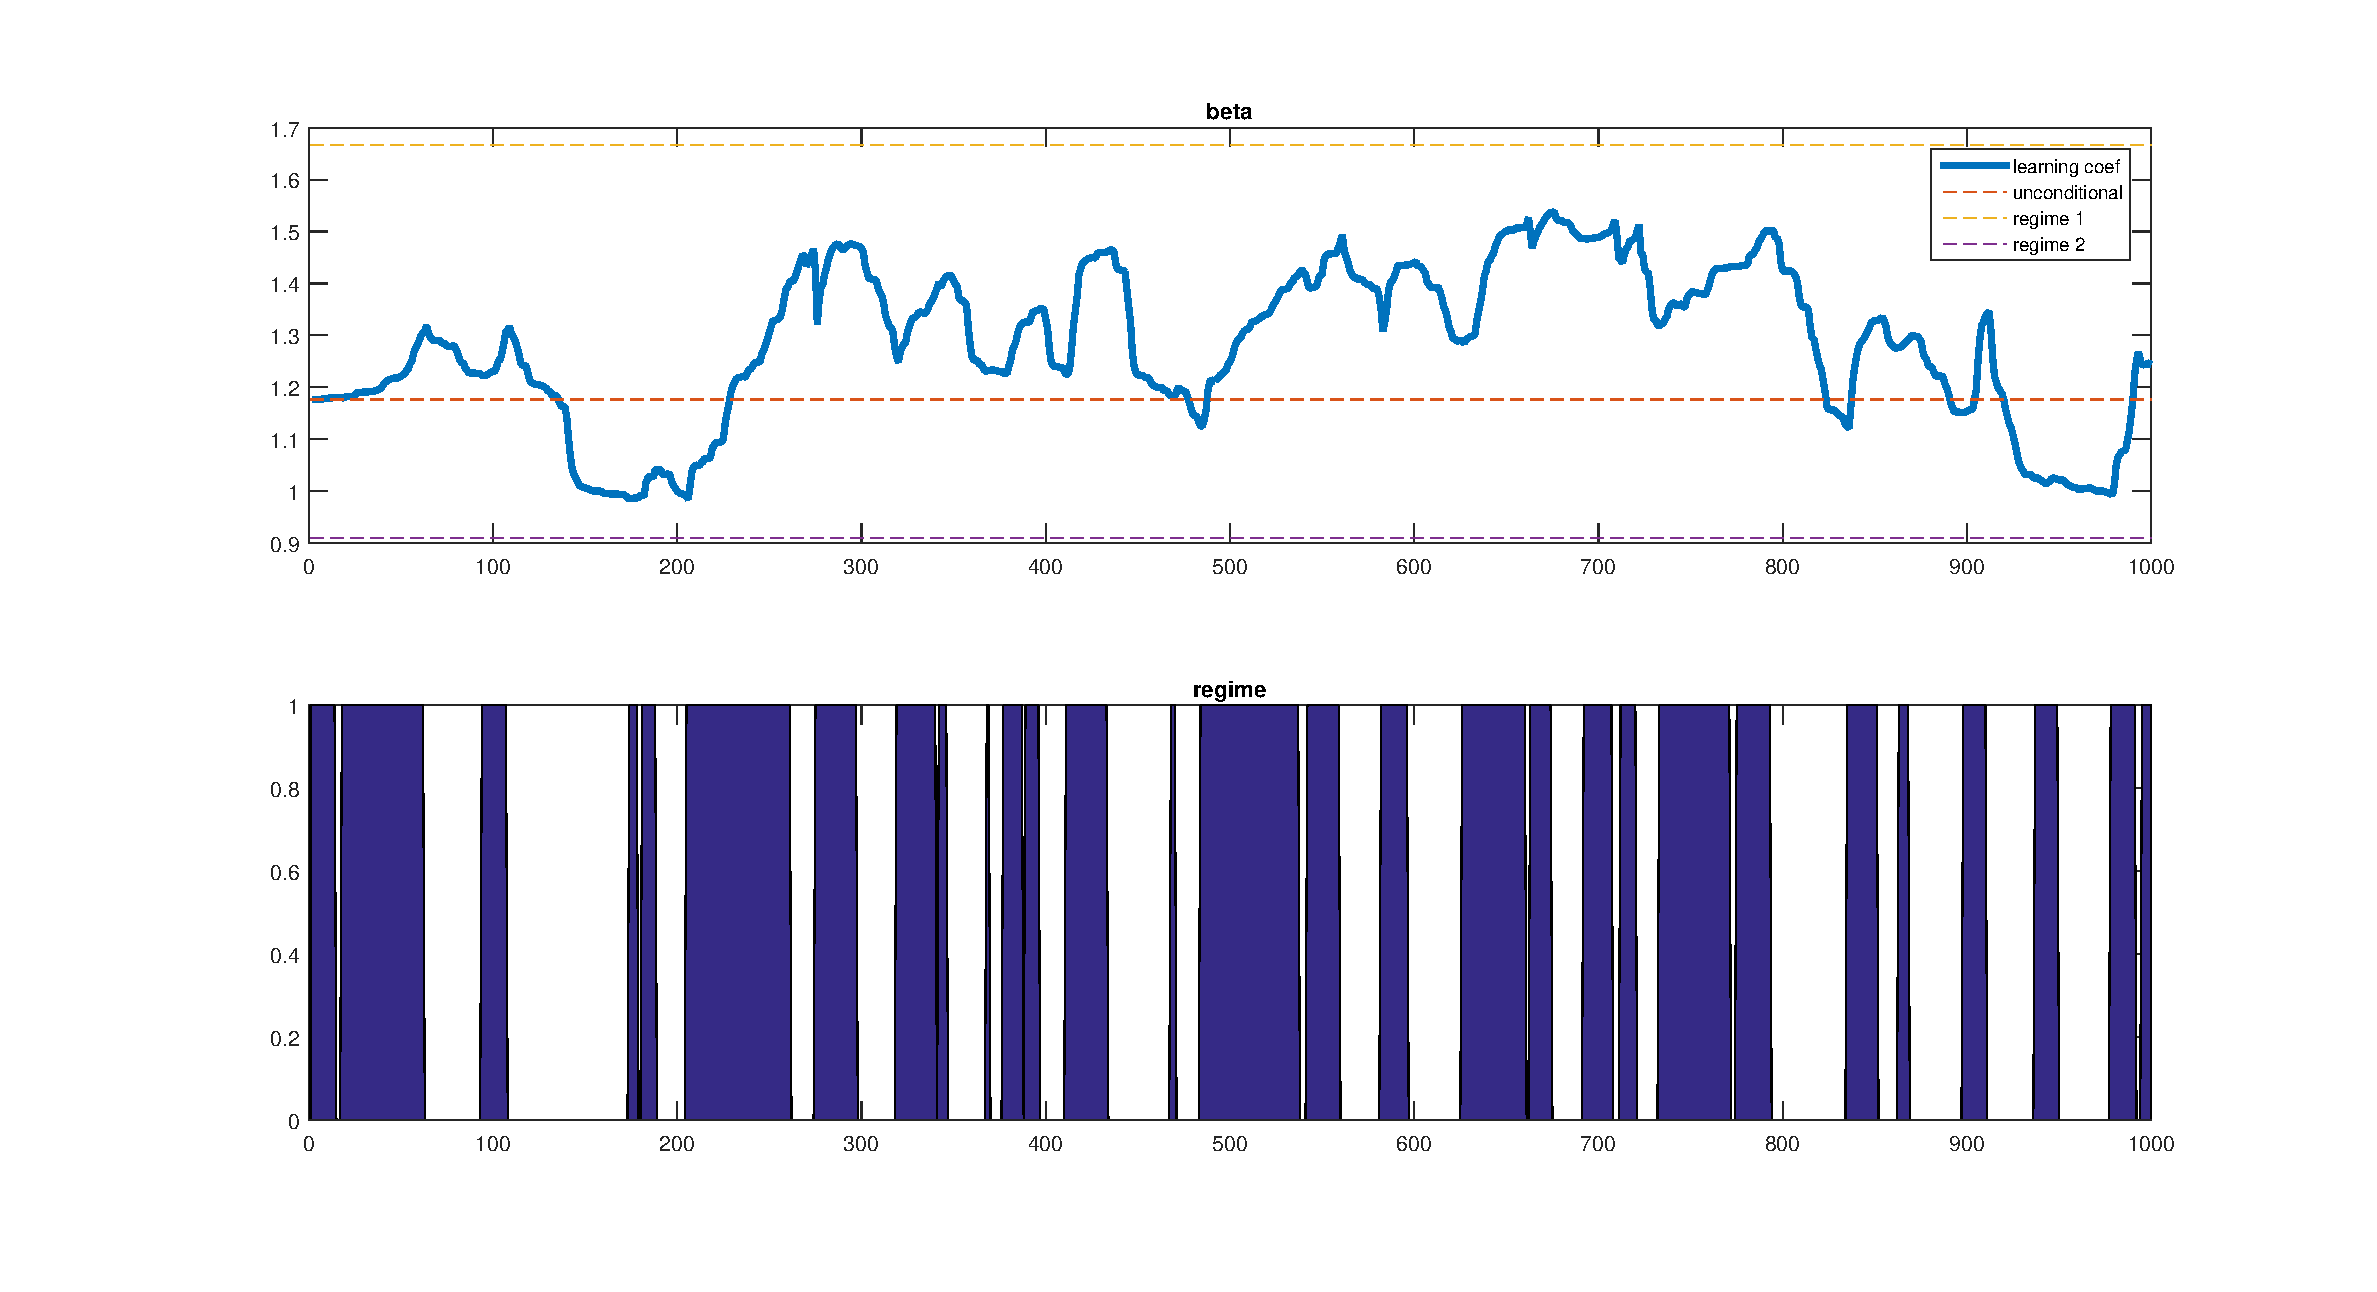
\includegraphics[scale=0.2]{fisher_simulation1_learningCoef.pdf} 
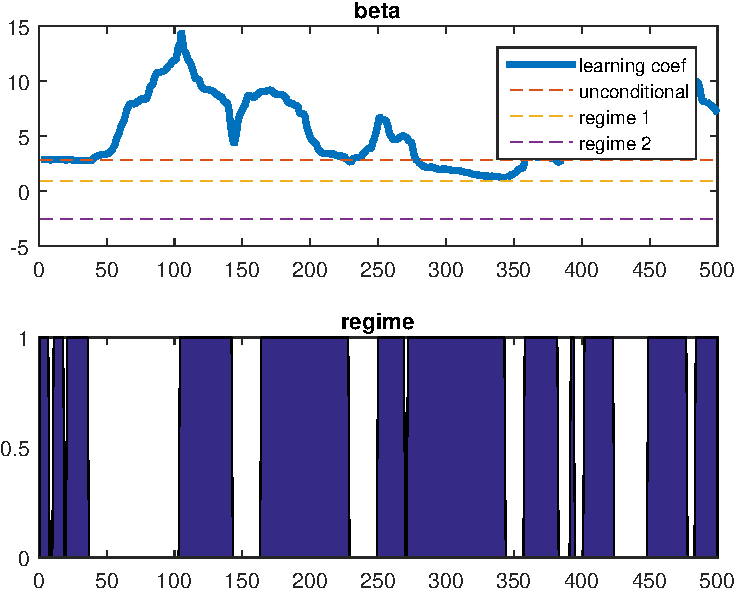
\includegraphics[scale=0.2]{fisher_simulation2_learningCoef.pdf} \\
%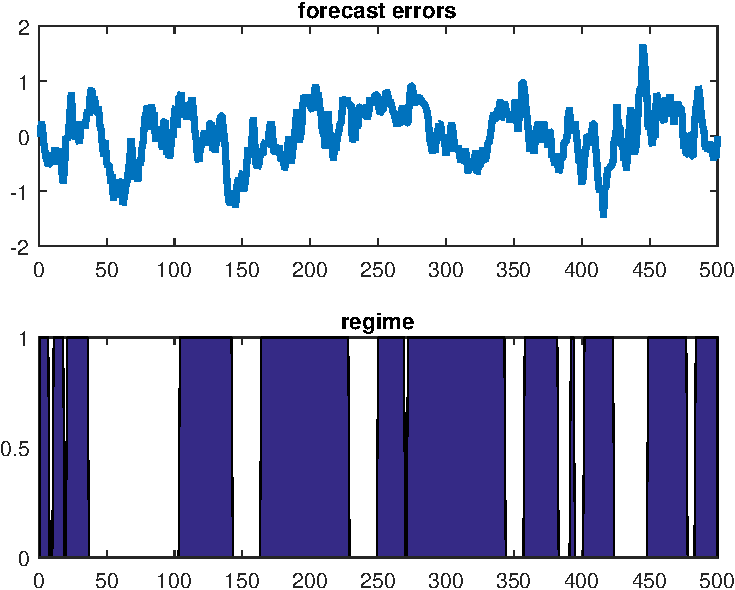
\includegraphics[scale=0.6]{fisher_simulation1_FE.pdf} \\


\textbf{Inflation:} \\

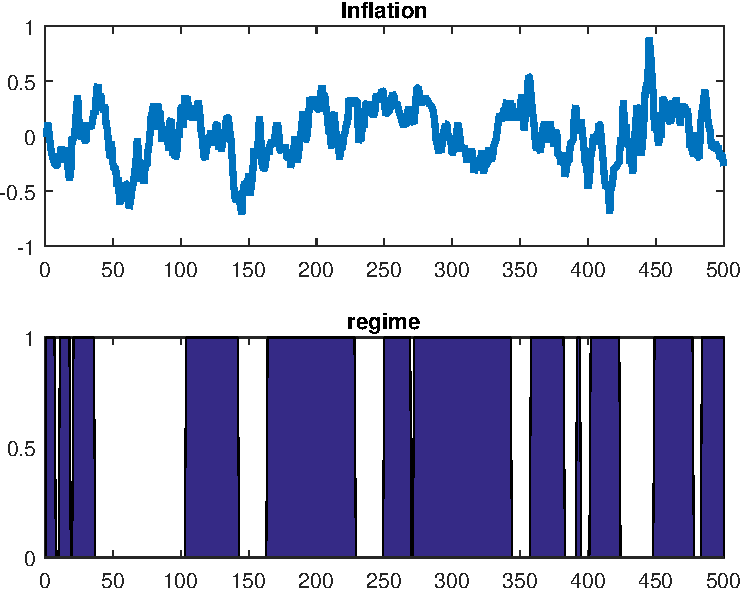
\includegraphics[scale=0.2]{fisher_simulation1_pinf.pdf} 
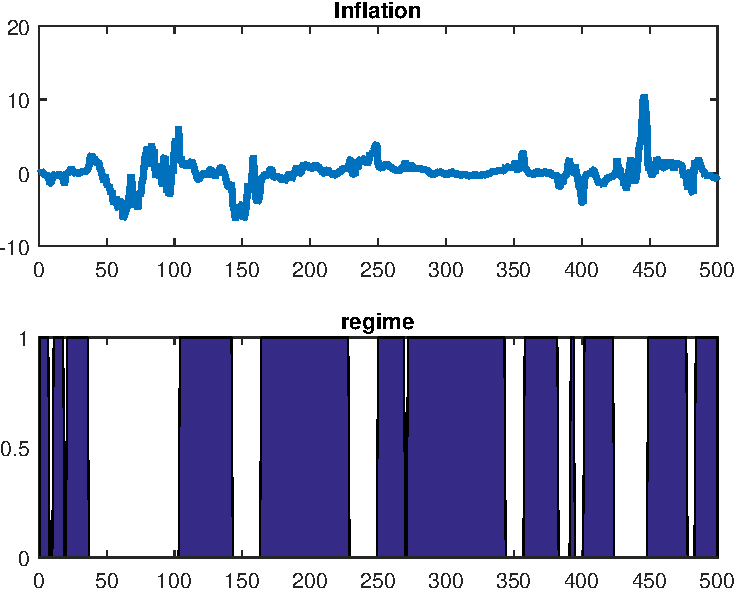
\includegraphics[scale=0.2]{fisher_simulation2_pinf.pdf} \\
\end{figure}

\section{Restricted Perceptions Equilibria in MS-DSGE Models: General Case}

Our simple example in the previous section illustrates well our idea of restricted perceptions in Markov-switching DSGE models, where we can analytically compute the Restricted Perceptions Equilibrium. In this section, we generalize our results to cases with multiple forward-looking variables, where the underlying equilibrium quickly becomes intractable. Accordingly, first consider the data generating process: \\

$$
\begin{cases}
X_t = A(s_t) + B(s_t) X_{t-1} + C(s_t) E_t X_{t+1} + D(s_t) \epsilon_t \\
\epsilon_t = \rho \epsilon_{t-1} + \eta_t 
\end{cases}
$$

where $X_t $ denotes the state-variables that depend on their lags, 1-step ahead expectations and the structural shocks $\epsilon_t$, which itself follow a VAR(1) process. We assume that the corresponding matrices A, B, C and D contain structural parameters subject to regime switches captured by $s_t$.  We consider two benchmark cases for the information set (i.e. the PLM) of the agent and the corresponding 1-step ahead expectations: the first one assumes that agents PLM coincides with the form of the underlying MSV-solution, except that the regime-shifts are not taken into account. In the second case, we consider the more general VAR(1)-type learning rules, which assumes observed shocks and the cross-correlations may be misspecified.  


\subsection{MSV-consistent RPE} 

First assume that PLM takes the form of the MSV-solution but is not regime-contingent. Accordingly, the PLM and expectations take the following form: \\

$$
\begin{cases}
X_t = a + b X_{t-1} + d \epsilon_t \\
E_t X_{t+1} = (a+ba) + b^2 X_{t-1} + (bd + d\rho) \epsilon_t 
\end{cases}
$$

where we assume that structural shocks are contemporaneously observed while the state-variables are not. Plugging this back into the ALM yields the implied ALM: 


$$
X_t = ( A(s_t) + C(s_t) (a+ba) ) + (C(s_t) b^2 + B(s_t))X_{t-1} + ( C(s_t) (bd +d \rho ) + D(s_t) ) \epsilon_t 
$$

For the remainder, we use the notation $\tilde{m} = \sum_i q_i m_i $ for the weighted average of any matrices $m_i $. Imposing the moment restrictions in this case yields: \\

$$
\begin{cases}
a = E[ A(s_t) + C(s_t)  (a+ba)]= \tilde{A} + \tilde{C} (a+ba) \\
b=E[C(s_t) b^2 + B(s_t)]=\tilde{C} b^2 + \tilde{B} \\
d = E[C(s_t) (bd+d \rho) + D(s_t)] = \tilde{C} (bd + d \rho ) + \tilde{D} 
\end{cases}
$$

In the above expression, a and d can be obtained for a given b. However, the second equation is quadratic in b. With n endogenous variables, this can in principle have up to $ {2n}\choose{n} $ solutions in b (Evans \& Honkapohja, (??)). Note, however, that in this special case the underlying RPE is simply the weighted average of the regime-specific MSV solutions, hence the fixed-point can be computed using standard methods such as Uhlig (??). 

In this case, the T-map is given by: \\

$$
\begin{pmatrix} a \\ b \\ d \end{pmatrix} \rightarrow \begin{pmatrix} \tilde{A} + \tilde{C} (a+ba) \\ \tilde{C} b^2 + \tilde{B} \\  \tilde{C} (bd+d \rho) + \tilde{D} \end{pmatrix}
$$

Denoting $\theta = (a,b,d)' $, the associated Jacobian is : \\

$$ \frac{ D T } { D\theta }  = \begin{bmatrix} \tilde{C} + \tilde{C} b & vec_{n,n}^{-1} (a' \otimes \tilde{C}) & 0 \\
0 & 2 \tilde{C} b & 0 \\
0 & vec_{n,n}^{-1}(d' \otimes \tilde{C} ) & \tilde{C} b + vec_{n,n}^{-1} (\rho' \otimes \tilde{C} ) \end{bmatrix} $$

where $ vec_{n,n}^{-1} $ denotes the matricization of a vector to an $(n,n) $ matrix. \\

The eigenvalues of the Jacobian above are given by the terms on the diagonal. Hence the underlying RPE is E-stable if these eigenvalues have real parts less than one. \\

%(these eigenvalues include the $ b $ term itself, i.e. $b $ will converge to something if $b $ satisfies a certain condition. Does this make sense? Cars' paper had something similar and the referees didn't like it, is it the same thing? ) \\





\subsection{VAR-consistent RPE} 

So far we considered MSV-type of learning, where the only source of misspecification in PLM comes from the fact that expectations are not regime-specific. In general, however, we can consider any type of misspecification in the PLM and there may exist an E-stable RPE associated with the given PLM. In this section, we extend our analysis to VAR(1)-type rules with unobserved shocks. 
Accordingly, consider again models of the form:

$$
\begin{cases}
X_t = A(s_t) + B(s_t) X_{t-1} + C(s_t) E_t X_{t+1} + D(s_t) \epsilon_t \\
\epsilon_t = \rho \epsilon_{t-1} + \eta_t 
\end{cases}
$$

Since shocks are assumed to be unobserved, we can stack up the endogenous variables $X_t $ and exogenous shocks $\epsilon_t $ into a vector $ S_t = [X_t' \hspace{3 mm}\epsilon_t']' $ to obtain models of the form: \\

$$
S_t = \gamma_0 (s_t) + \gamma_1 (s_t) S_{t-1} + \gamma_2(s_t) E_t S_{t+1}  + \gamma_3 (s_t) \eta_t
$$

Assume the PLM, and the one-step ahead expectations take the form: \\

$$
\begin{cases}
S_t = a + b S_{t-1} + u_t \\
E_t S_{t+1} = (a+ba)+ b^2 S_{t-1} 
\end{cases}
$$

Implied ALM is given by: \\

$$ 
S_t = (\gamma_0 (s_t) + \gamma_2 (s_t) (a+ba))+ (\gamma_1 (s_t) +\gamma_2 (s_t) b^2 )S_{t-1} + \gamma_3(s_t) \eta_t 
$$

In cases where the matrix $b $ does not exactly coincide with the functional form of the MSV solution, the consistency requirements do not simplify. \\

$ E [ S_t ] = (I-b)^{-1} a  $ in PLM.  \\

$ E [S_t] = ( I -  \tilde{\gamma_1} - \tilde{\gamma_2} b^2 )^{-1} (\tilde{\gamma_0} + \tilde{\gamma_2}(a+ba)  ) $ in ALM. \\

The vector $ a $ in the expression above can be solved for a given $ b $. Next we turn to the consistency requirement for the matrix $ b $. Note that in PLM, we have : \\

$ E [ \tilde{S_t} \tilde{S_t}']^{-1} E [ \tilde{S_t} \tilde{S_{t-1}}'] = b $, where $\tilde{S_t} = S_t - E[S_t]$. Hence we turn to computing these moments in ALM. Denoting by $\Gamma_0 $ and $\Gamma_1 $ the variance and autocovariance matrices respectively, the first two Yule-Walker equations of the ALM are given as : \\

$$
\begin{cases}
\Gamma_1 = \tilde{M}(b) \Gamma_0 \\
\Gamma_0 = \tilde{M}(b) \Gamma_0 \tilde{M}(b)' + \tilde{\gamma_3}\Sigma_{\eta} \tilde{\gamma_3}' 
\end{cases}
$$

where $\tilde{M}(b) = \tilde{\gamma_1} + \tilde{\gamma_2} b^2$. Solving the second expression above yields 
$$ vec(\Gamma_0) = (I- \tilde{M}(b) \otimes \tilde{M}(b))^{-1} (\tilde{\gamma_3} \otimes \tilde{\gamma_3}) vec(\Sigma_{\eta}) $$

Hence for each term $b(i,j) $, we have $ b(i,j) = \frac{vec(\Gamma_1)_{(j-1)N+j}}{vec(\Gamma_0)_{(j-1)N+j}} \Rightarrow b = \Gamma_1 \oslash \Gamma_0 $. \\

In the special case where $ b $ takes the form of the corresponding MSV matrix on lagged endogenous terms, the solution for $ b $ reduces to the quadratic equation $ b = \tilde{\gamma_1 } + \tilde{\gamma_2 } b^2 $ as in the previous case. \\

The T-map in this case is given by the following: \\

$$
T: \begin{pmatrix} a \\ b \end{pmatrix}  \rightarrow \begin{pmatrix} \tilde{\gamma_0} + \tilde{\gamma_2} (a+ba) \\ \tilde{\gamma_1} + \tilde{\gamma_2} b^2 \end{pmatrix} 
$$

Denoting $ \theta = (a,b) $ , the corresponding Jacobian is \\

$$
\frac{DT}{ D \theta} = \begin{bmatrix}  \tilde{\gamma_2 } (I+b) & vec^{-1}_{n,n} ( a' \otimes \tilde{\gamma_2}) \\ 0 & 2 b \tilde{\gamma_2}  \end{bmatrix} 
$$
Hence the corresponding RPE will be E-stable if the eigenvalues $\tilde{\gamma_2} (I+b) $ and $ 2 b \tilde{\gamma_2} $ have real parts less than one. \\


\subsection{Illustration: Constant-gain Least Squares in the 3-eqution NKPC}
(add the interest rate smoothing into policy rule)\\

In general, we do not explicitly compute the expressions for the MSV- and VAR-consistent RPE respectively. However, the presence of these RPE and their E-stability under general conditions allows us to conclude that the Markov-switching models under adaptive learning are going to oscillate around an ergodic distribution, rather than showing explosive behaviour. Accordingly, one might expect the models to be stationary under the standard least-squares learning given by: \\


$$
\begin{cases}

R_t = R_{t-1} + \gamma (S_{t-1}^2 - R_{t-1} ) \\
\theta_t = \theta_{t-1} + \gamma R_t^{-1} S_{t-1} (S_t - \theta_{t-1} S_{t-1}) 
\end{cases}
$$

where $\theta_t$ and $R_t$    denote the set of learning coefficients and their estimated covariance matrix respectively.  

Now consider the baseline 3-equation NKPC model along the lines of Woodford (2003), where the interest rate is subject to the ZLB constraint: \\

$$
\begin{cases} 
x_t = E_t x_{t+1}  -\frac{1}{\tau}(r_t - E_t \pi_{t+1})+ \epsilon_{x,t} \\
\pi_t = \beta E_t \pi_{t+1} + \kappa x_t + \epsilon_{\pi,t} \\
r_t = max\{ 0, \rho r_t+(1-\rho) (\phi_x x_t + \phi_{\pi} \pi_t )+ \eta_{r,t}\} \\
\epsilon_{y,t} = \rho_y \epsilon_{y,t-1} + \eta_{y,t} \\ 
\epsilon_{\pi,t} = \rho_{\pi} \epsilon_{\pi,t-1} + \eta_{\pi,t} \\
\end{cases} 
$$

We can re-cast the interest rate rule above as a Markov process with two regimes, where: \\

$$
\begin{cases}
r_t (s_t=1) = \rho r_{t-1} +(1-\rho) (\phi_x x_t + \phi_{\pi} \pi_t) + \eta^{1}_{r,t}\} 
r_t (s_t=2) =\eta^{2}_{r,t}\} 
\end{cases}
$$

with the same transition matrix same as in the first example. The presence of noise in the second regime is meant to capture the fact that, although interest rates are very close to zero in empirical data, they are never exactly equal to zero in the post-2007 period (Binning et al (??)). In this form, the example essentially extends the results of the previous example to the multi-dimensional case. We simulate the model 500 times, each with length 10000 under the calibration $\phi_y =0.5, \phi_{\pi}=1.5, \rho=0.9, \kappa=0.01, \beta=0.99, \sigma_y = 0.7, \sigma_{\pi} =0.3, \sigma^{I}_r =0.3, \sigma^{II}_r=0.01,\rho_y =0.5, \rho_{\pi}=0.5 , p_{11} = 0.99, p_{22} = 0.9, \gamma = 0.01$, hence the ZLB regime has an expected duration of 10 periods. A standard result in the literature is that, under plausible parameter values, the normal regime is E-stable while the ZLB regime is not (Evans \& Honkapohja (??)), which also applies to our calibration here. Since the expected duration of the ZLB period is set to a low value, however, one may expect the underlying RPE to be E-stable. We check this by the following Monte-Carlo study: we consider the model under constant-gain least-squares with the first case of MSV-type PLM. We simulate the model 500 times each with length 10000, and we collect the final values of the learning coefficient in PLM. The corresponding histograms are shown in Figure (??): the resulting distributions for all variables have a clear peak, suggesting the underlying RPE is indeed E-stable and the constant-gain learning oscillates around this fixed-point. Similar results can also be obtained under a constant-gain VAR(1) learning, which we omit here and move onto the estimation of Markov-switching models under adaptive learning. 

\begin{figure}[H]
\caption{Distributions from 500 simulations of length 10000 for the two-regime NKPC. First row: intercept terms (should converge to zero). Second and third rows: lagged inflation and output gap coefficients (should converge to zero as they do not belong in the MSV-rule). Fourth row: Lagged interest rate: should converge to non-zero values given non-zero interest rate smoothing. Fifth and sixth rows: Coefficients on output gap and inflation shocks: should converge to non-zero values. Overall, we observe similar distributions compared to the switching (and also non-switching) case of previous section, indicating convergence towards an equilibrium. }
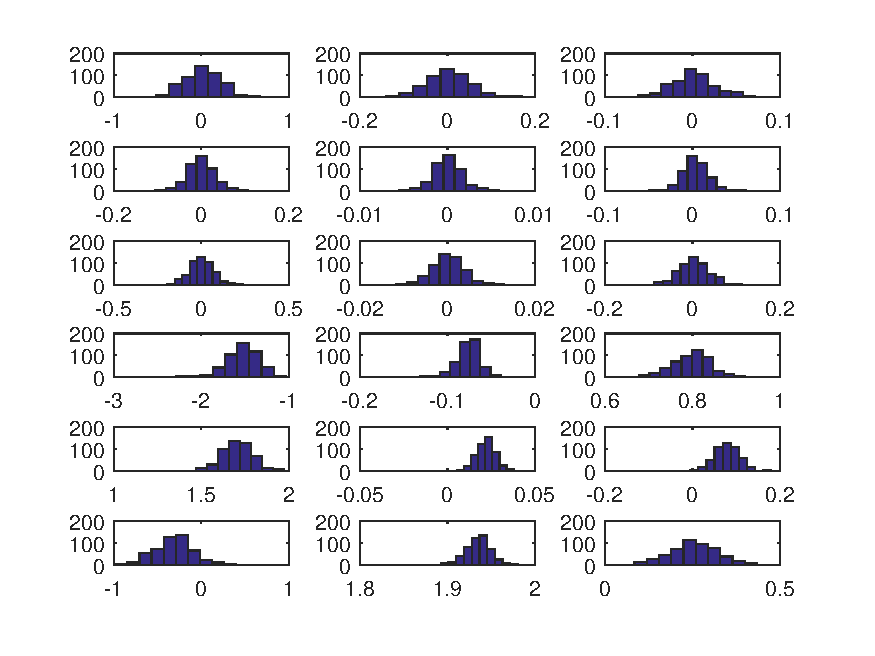
\includegraphics[scale=1]{MC_MS_MSV_withLags.pdf}\\
\end{figure}




\section{Bayesian Estimation of Markov-Switching DSGE Models under Adaptive Learning: Filtering Algorithm }


The benchmark algorithm for Markov-switching state-space models is the Kim \& Nelson (1999) filter (henceforth KN-filter): in a Markov-switching model with $m $ distinct regimes, a dataset of size $T$ leads to $m^T$ distinct timelines, which quikcly makes the standard Kalman filter intractable. The KN-filter introduces the so-called \textit{collapsing} technique to deal with this issue, which amounts to taking weighted averages of the state vector and covariance matrix at each iteration of the filter. This effectively reduces the number of timelines at each iteration by an order of $m$, thereby making the filter tractable again. The standard recommendation is to carry as many lags of the states as appears in the transition equation. Therefore, given that we consider we consider DSGE models that have a reduced-form VAR(1) representation, we carry only a single lag of the state variables, meaning if there are $ m $ different regimes in the model, we carry $m $ different timelines in each period. Therefore there are $m^2$ different sets of variables in the forecasting and updating steps of each iteration. These are then collapsed at the end of each iteration to reduce to $m $ sets of variables. \\
\noindent
An important question is how to introduce adaptive learning into this framework. We adapt an approach that consistent with the theoretical framework of the previous period: the agents have a unique PLM based on observables, independent of the regime switches. We model this formally by collapsing the $m $ different states further at each iteration to obtain the \textit{filtered states}, which are then used to carry out the adaptive learning step. The uniquely updated steps are then used in each distinct timeline of the following iteration\footnote{A natural alternative here is to apply the adaptive learning step distinctly to each collapsed state; one can then take a weighted average of these expectations to obtain the \textit{filtered expectations}. Our results in the upcoming sections do not change substantially if we use such an alternative, but we use the first approach since it is more in the spirit of our theoretical framework.} 




State-space representation of the model, where $S_t $ and $y_t $ denote (unobserved) states and observable variables respectively: \\


\begin{table}[H]
\noindent\rule{\textwidth}{1pt}
\textbf{KM-filter for Markov-Switching DSGE Models under Adaptive Learning}\\
\noindent\rule{\textwidth}{1pt}
$$
\begin{cases}
S_t = \gamma_2 + \gamma_1 S_{t-1} + \gamma_3 \epsilon_t, \hspace{3 mm}, \epsilon_t \sim N(0, \Sigma) \\
y_t = E+ F S_t \\
\end{cases}
$$

\noindent\rule{\textwidth}{1pt}

\underline{0) Initial  States :}

$ \tilde{S}_{0|0}^{i}, \tilde{P}_{0|0}^{i}, Pr[ S_0=i | \Phi_0] , \Phi_0$  given.\\
%\vspace{3 mm}
\noindent\rule{\textwidth}{1pt}

\noindent
\underline{1) Kalman Filter Block with the standard measurement and transition equations:} \\
%\vspace{3 mm}
For $t=1:N$\\
    For $\{S_{t-1}=i, S_t=j\} $
\noindent
$$
\begin{cases}
S_{t|t-1}^{(i,j)}=\gamma_1^{(j)} S_{t-1|t-1}^{(i)} + \gamma_2^{(j)} \\
P_{t|t-1}^{(i,j)}=\gamma_1^{(j)} P_{t-1|t-1}^{(i)} \gamma_1^{(j)} + \gamma_3^{(j)} \Sigma^{(j)} (\gamma_3^{(j)})^{\prime} \\
v^{(i,j)}_{t|t-1} = (y_t - F^{(j)} S_{t|t-1}^{(i,j)})\\
Fe^{(i,j)}=F^{(j)} P_{t|t-1}^{(i,j)}F^{(j)} \\
S_{t|t}^{(i,j)}= S_{t|t-1}^{(i,j)} + P_{t|t-1}^{(i,j)} (F^{(j)})^{\prime} {(Fe^{(i,j)})}^{-1} v^{(i,j)} \\
P_{t|t}^{(i,j)} = P_{t|t-1}^{(i,j)} (F^{(j)})^{\prime} (Fe^{(i,j)})^{-1} F^{(j)} P_{t|t-1}^{(i,j)} \\
\end{cases}
$$

\vspace{5 mm}
\noindent\rule{\textwidth}{1pt}
\noindent
\underline{2)  Hamilton Block for transition probabilities:}\ \\
%\vspace{3 mm}

\noindent
Denote: $ Pr[S_{t-1}=i,S_t=j | \Phi_{t-1} ] = pp_{t|t-1}^{i,j} $,$f(y_t|\Phi_{t-1}) $ the marginal likelihood,\\ $Pr[S_{t-1}=i,S_t=j|\Phi_t]= pp_{t|t}^{i,j} $ and  $Pr[S_t=j|\Phi_t]= \tilde{pp_{t|t}^{j}}$.
%\vspace{2 mm}

$$
\begin{cases}
pp_{t|t-1}^{(i,j)}=Q(i,j) pp_{t-1|t-1}^{(i)} \\
f(y_t|\Phi_{t-1}) = \sum_{j=1}^M \sum_{i=1}^M f(y_t | S_{t-1}=i, S_t=j, \Phi_{t-1} ) pp_{t|t-1}^{(i,j)} \\
pp_{t|t}^{(i,j)} = \frac{f(y_t | S_{t-1} = i, S_t = j, \Phi_{t-1}) pp_{t|t-1}^{(i,j)} } { f(y_t| \Phi_{t-1})} \\
p_{t|t}^{j} = \sum_{i}^M pp_{t|t-1}^{(i,j)}\\
\end{cases}
$$

\noindent\rule{\textwidth}{1pt}
\noindent
\underline{3) Collapsing to reduce the number of states from $m^2 $ to m:} \\
$$
\begin{cases}
{S}_{t|t}^{(i)} = \frac{\sum_{i=1}^M pp_{t|t}^{(i,j)} S_{t|t}^{(i,j)} } { p_{t|t}^{(j)}} \\
{P}_{t|t}^{(i)}= \frac{\sum_{i=1}^M pp_{tt}^{(i,j)} (P_{t|t}^{(i,j)} + (S_{t|t}^{(j)} - S_{t|t}^{(i,j)})(S_{t|t}^{(j)} - S_{t|t}^{(i,j)})^{\prime})}{p_{t|t}^{(j)}}
\end{cases}
$$
%\vspace{1 mm}

\noindent\rule{\textwidth}{1pt}
\noindent
\underline{4) Update expectations based on filtered states:} \\
%\vspace{3 mm}

\textbf{Updating Expectations based on Filtered States:}
$$
\begin{cases}
\tilde{S}_{t|t} = \sum_{j=1}^M p_{t|t}^{(j)} S_{t|t}^{(j)}\\
\Phi_t = \Phi_{t-1} + \gamma R_t^{-1} \tilde{S}_{t-1|t-1}(\tilde{S}_{t|t}- \Phi_{t-1}^{T} \tilde{S}_{t-1|t-1})^{T} \\
R_t^{-1} = R_{t-1} + \gamma (\tilde{S}_{t-1|t-1}\tilde{S}_{t-1|t-1}^{T} - R_{t-1}) \\
\end{cases}
$$

\end{table}


\subsection{Initial Beliefs}

The first practical issue with the above filter is Step (0), i.e. where to initialize the beliefs. This has been shown to play a key role in driving the estimation results in previous studies, and various different approaches have been considered: Milani (??) uses an estimation-based approach, where the initial beliefs are treated as structural parameters and estimated jointly along with the other parameters of interest; Slobodyan \& Wouters (2012a, 2012b??) consider REE-based and training-sample based approaches along with the estimation-based approach; and Galimberti (??) proposes a smoothing-based approach. A common result in these studies is that  the results are sensitive to initial beliefs, and the best-fitting approach typically depends on the specific model under consideration. \\
\noindent
In this paper, following Slobodyan \& Wouters (??), we present our main results under the REE-based initial beliefs and check the sensitivity of these results to alternative specifications. Accordingly, as our main approach, we estimate the benchmark (non-switching) REE, and use the relevant moments implied by the matrices $\gamma_1$ and $\gamma_3$ from this estimation in the initialization step  of the learning models\footnote{The REE-implied intercepts are always zero, therefore the vector $\gamma_2$ is always initialized at the vector of zeros}. As our alternatives, we consider three approaches: (i) training-sample approach, where we initialize the filter at diffuse moments and estimate it on a training sample\footnote{For both models considered in the latter sections, our training sample is based on pre-1966 period of aggregate U.S. variables.}, then use the final values of the learning coefficients to initialize the main estimation; (ii) estimation-based approach, where we first estimate all belief coefficients jointly with the structural parameters in a VAR model, then use the resulting estimates to initialize the main estimation; (iii) a filter-based approach, where, at each step of the estimation, the beliefs are initialized at diffuse points and ran once, then the converged values of the belief coefficients are used as initial values to run the filter for a second time. The results of the alternative estimations are provided in the Appendix, and while the relative fit of each model is indeed sensitive to the initial beliefs, our main conclusions continue to hold in all specifications. 

\subsection{Projection Facilities} 

The second practical issue with the above filter is how to retain the stability of the underlying model with adaptive learning. In most operational macro models, the MSV-solution includes lagged state variables due to properties such as habit formation, indexation in prices and wages, interest rate smoothing, etc. When these parameters in PLM are updated each period in a constant gain setup, they may easily end up in an unstable region, which then feeds back into the implied ALM and leads to explosive dynamics. Models subject to the zero lower bound constraint are more prone to encounter this problem, since typically an inactive monetary policy  rule implies indeterminacy and E-unstability for the regime-specific dynamics. A common way in the adaptive learning literature to deal with these potential instabilities is to impose a so-called projection facility on the model, which projects the learning parameters into a point in the stable region when the instability is encountered. One simple approach to do this is to leave the parameters at their previous value if the update leads to an instability, which is the approach adopted in Slobodyan \& Wouters (??). In this paper we use a variant of this simple idea: we stop updating the learning parameters each period, if the update pushes the largest eigenvalue of the system outside the unit circle. We base our notion of stability on the ergodic distribution of the Markov chain: the model is said to be explosive at any set of parameter values, if the largest eigenvalue of the ergodic distribution is outside the unit circle. Accordingly, we allow the regime-specific models to be explosive, as long as the underlying distribution is still stable. This approach does not have an impact on our estimation of the small-scale NKPC since we do not encounter unstable regions in this case; but it plays an important role in the estimation of medium-scale SW model as we show in the upcoming sections. 








\section{Estimation of the 3-equation NKPC} 

In this section, as a first step, we estimate the small-scale 3-equation NKPC model presented in the previous section. In this framework there are 18 parameters to be estimated, to which we assign prior distributions consistent with the previous literature: the slope of Phillips curve is assigned a Beta distribution centered at $0.3$ with a standard deviation of $0.15$, while the risk aversion coefficient has a gamma distribution with a mean 2 and standard deviation $0.5$; these are directly taken from (??). The monetary policy reaction coefficients are given Gamma distributions centered at $1.5$ and $0.5$ respectively, with a standard deviation of 0.25; these are the standard values associated with the Taylor rule. Interest rate smoothing, shock persistence and shock standard deviation coefficients are consistent with Smets \& Wouters (2007), the first two having a Beta distribution with mean $0.5 $ and st. dev $0.2$, while the latter is assigned a Gamma distribution with mean $0.1$ and st. dev 2. The regime probabilities are taken from Binning et al (2017): the exit probability of the normal regime is a Beta distribution with mean $0.1$ and standard deviation $0.05$, while the exit probability of ZLB regime is a Beta distribution with a mean $0.3$ and st. dev $0.01$. The gain coefficient follows the same distribution as in Slobodyan \& Wouters (2012) with a gamma distribution and a mean of $0.035$, but we assume a tighter distribution with a standard deviation of $0.015$. The steady-state level of interest rate at the ZLB regime is given a normal distribution with a mean and st. dev of $0.1$ and $0.25$ respectively, while the policy shocks at the ZLB regime are assumed to follow a uniform distribution with a mean and st. dev of $0.005$ and $0.05$ respectively.\\
\noindent
We use quarterly U.S. data over the period 1966:I-2016:IV on interest rates, inflation and output gap with the following simple measurement equations: 
$$
\begin{cases}
y_t^{obs}=\bar{y}+y_t \\
\pi_t^{obs}= \bar{\pi} + \pi_t \\
r_t^{obs}=\bar{r}+r_t 
\end{cases}  
$$

where the mean parameters $\bar{y}, \bar{\pi} $ and $\bar{r}$ are assigned normal distributions based on the pre-1966 period. \\

Table \ref{nkpc_estimation} shows the point-estimates for five model specifications: for the constant-gain learning cases, we consider a univariate AR(1) rule, a VAR(1) rule including output gap, inflation and interest rates, and the MSV-type rule that assumes regime switches are unobserved as discussed above. The last two columns show the two benchmark Rational Expectations cases with and without regime switching\footnote{The REE-MS specification is estimated using J. Maih's RISE toolbox, while the standard REE case is obtained from the Dynare toolbox. For the adaptive learning specifications, we use our filter as presented in the previous section. Note that RISE toolbox uses a variant of the same KN filter, hence the estimations are based on the same filter except for the adaptive learning component.}. First looking at the resulting likelihoods based on Laplace approximation, we see an expected pattern: the MS-REE model leads to a substantial improvement over the benchmark REE model, implying that the regime shift on interest rates plays an important role in driving the model fit. Further adding adaptive learning on top of Markov-switching improves the likelihood further: all three adaptive learning specifications outperform the REE-MS model. Both of these results, individually, are consistent with the previous results found in the literature, i.e, it is well known that both Markov-switching and adaptive learning typically improve the model fit compared with the benchmark case. Our contribution here is to put these two results together.\\
\noindent
Next we turn to the discussion of our parameter estimates: the results under REE-MS are generally similar to the REE model with the exception of the risk aversion parameter $\tau$, which is lower under REE-MS with $2.75 $ compared with $4.57 $ under REE. Comparing the MSV-learning case to REE-MS, the differences are minimal: The only differences arise in the interest rate smoothing $\rho_r$ and output gap reaction $\phi_y$ and the the risk aversion  coefficient $\tau$, which turn out slightly higher under MSV-learning. Another difference is the exit probability from ZLB regime, which is estimated to be lower under MSV-learning. At the estimated coefficients, this implies the ZLB regime has an expected duration of  5.9 quarters under MS-REE, while this is 7.69 under MSV-learning. In other words, the estimated persistence of the ZLB regime is higher under the learning specification. These differences become more pronounced as we move onto the AR(1) and VAR(1) cases: the exit probability from ZLB regime under AR(1)-learning is the same as in MSV case with an expected duration of 7.69, while the ZLB regime is even more persistent under VAR(1)-learning with an expected duration of 9.1 quarters. These results show that, in general, the expected duration of the ZLB regime is much larger under any type of learning compared with the MS-REE case. Further, in both AR(1) and VAR(1) cases, the NKPC slope $\kappa$ is substantially larger at 0.036 and 0.029 respectively, compared with 0.005, 0.004 and 0.006 under MSV-learning, REE-MS and REE cases: this is a direct consequence of assuming unobserved shocks, which shifts the transmission channel from expectations to the parameter $\kappa$. Another important difference between AR(1) and VAR(1) compared with the remaining specifications is the shock persistence terms: in both cases, the persistence of shocks are much smaller compared with the remaining cases. This results from the backward-looking nature of AR(1) and VAR(1) rules, which shift some of the exogenous persistence in the shocks onto expectations, thereby resulting in lower estimates for the shock persistences. Furthermore, the gain coefficient increases as we reduce the information set: it is lowest for the MSV-learning case and highest for the univariate AR(1) rule. Among the three learning rules, the most parsimonious AR(1) rule yields the best fit with a Laplace approximation of -273, while the VAR(1) rule yields the worst one with -303. \\
\noindent
Figure \ref{nkpc_regime_prob} shows the filtered regime probabilities for the AR(1)-learning RS-REE cases along with the historical interest rates over the estimation sample. Is is readily seen that the estimated regime probability sharply rises in both cases in 2009 as the interest rates are lowered to near-zero levels. Both models indicate that towards the end of 2016, the economy is out of the ZLB regime as the interest rates slowly start to increase. The same pattern can be observed in the other cases of VAR(1)- and MSV-learning, which we omit here. This figure suggests that there are no differences in the estimated pattern of entering and exiting the ZLB regime, which is intuitive since the learning process should not have an impact on this. We next turn to the time variation in the belief coefficients over the estimation sample, which is shown in Figure \ref{nkpc_learning_coef} for all three learning cases. The most important difference arises in the pattern of intercept coefficients for MSV-learning with observed shocks, and AR(1) \& VAR(1) learning with unobserved shocks: while there is considerable time-variation in the intercept parameters in the latter cases, these is much less variation for MSV-learning. This suggests that when the exogenous shocks are assumed to be observed, the changes in the endogenous variables are attributed to these shocks and to changes in the feedback coefficients from exogenous shocks to endogenous variables. When the shocks do not enter into agents' information set, they attribute more changes to the time-variation in the intercept terms. In the AR(1) case, there is a sudden drop in the intercept terms during the 2007-08 crisis period, and these coefficients remain there during the remainder of the sample. The same observation also applies to the VAR(1) case, where the intercept of interest rates is also characterized with a sudden drop along with inflation and output gap. This suggests that there was a level shift in the agents beliefs for the endogenous variables during this period. This level shift does not arise in the MSV-learning case since the changes are attributed to the exogenous shocks. Accordingly, while all learning specifications provide a plausible characterization of the economy since they provide a better fit than the REE models, there is considerable difference in the implied evolution of beliefs during the sample period. This in turn suggests there might be important differences in how the economy responds to the same shock under different specifications.  Figure \ref{nkpc_impulse} shows the impulse responses for all estimated models\footnote{Note that, due to time-variation in beliefs, the impulse responses are different each period under the adaptive learning specifications. Therefore for Figure \ref{nkpc_impulse}, we consider two \textit{representative} periods based on 2006Q1 and 2011Q1 for the impulses under normal and ZLB regimes respectively. We leave the analysis of the time-variation in the impulse responses for the Smets-Wouters model.}: we consider the responses to one unit supply and demand shocks $\eta_y$ and $\eta_{\pi}$ respectively. As one might expect, the AR(1) and VAR(1) cases are very similar, while there is virtually no difference between MSV-learning and MSV-REE cases. A positive supply shock is expansionary and inflationary under all specifications, and the impact is larger under the ZLB regime since monetary policy does not mitigate the impact of this shock. An important difference between the observed shock and unobserved shocks cases is how long the shock takes to "kick in": under MSV-learning and MS-REE cases, the effect is maximal on impact, and the difference between the normal and ZLB regimes is therefore also maximal on impact. On the contrary, under the AR(1) and VAR(1) cases the effect is more gradual and takes a few periods to reach its maximum impact, leading to a hump-shaped response. Therefore the difference between normal and ZLB regimes also takes several periods to become visible. The impact of a demand shock is inflationary in all regimes and specifications, hence there is no difference with regards to the impact of this shock on inflation. However, there are important differences with regards to output: in the ZLB regime, a demand shock is always expansionary but the impact is again more gradual in the unobserved shock cases, leading to a hump-shaped response. In the normal regime, a demand shock is always contractionary is the observed shock cases, while it is initially expansionary and only becomes contractionary after ~8 quarters in the unobserved shock cases. \\
\noindent
As the above discussion makes it clear, we can already observe some important differences in the estimations and the implied stochastic structure of the economy even in the 3-equation setup. This raises the question of whether the differences will carry over to a more realistic model setup, which we analyze in the next section in the Smets-Wouters (2007) model. 







\begin{table}[H]
\label{nkpc_estimation}
\caption{Estimation Sample: 1966:I-2016:IV based on the U.S data, where the observables are the output gap (based on CBO's historical estimates), inflation and interest rate.The Markov-switching REE model is obtained from RISE toolbox, while the standard REE case is provided by Dynare. The AR(1), VAR(1) and MSV-learning cases are based on our algorithm above. }

\vspace{3 mm}

\begin{tabular}{l||lll||l|l|l|ll}
Parameter & Prior &  &  & Posterior &  &  &  &  \\
 &  &  &  & AR(1) & VAR(1) & MSV & REE-MS & REE \\
\hline
\hline
 & Dist & Mean & St. Dev & Mode & Mode & Mode & Mode & Mode  \\
$\bar{y}$ & Normal & 0 & 0.25 & -0.26 & 0.06 & -0.32 & -0.17 & 0.24 \\
$\bar{\pi}$ & Gamma & 0.62 & 0.41 & 0.38 & 0.78 & 0.7 & 0.39 & 0.17 \\
$\bar{r_1}$ & Gamma & 1 & 0.25 & 0.84 & 1.42 & 0.84 & 0.68 & 1.11 \\
\hline
$\kappa$ & Beta & 0.3 & 0.15 & 0.036 & 0.029 & 0.005 & 0.004 & 0.006 \\
$\tau$ & Gamma & 2 & 0.5 & 2.41 & 2.7 & 3.08 & 2.75 & 4.57 \\
\hline
$\phi_{\pi}$ & Gamma & 1.5 & 0.25 & 1.48 & 1.52 & 1.56 & 1.56 & 1.42 \\
$\phi_y$ & Gamma & 0.5 & 0.25 & 0.4 & 0.4 & 0.45 & 0.27 & 0.27 \\
$\rho_r$ & Beta & 0.5 & 0.2 & 0.87 & 0.93 & 0.9 & 0.8 & 0.8 \\
\hline
$\rho_y$ & Beta & 0.5 & 0.2 & 0.30 & 0.44 & 0.89 & 0.92 & 0.93 \\
$\rho_{\pi}$ & Beta & 0.5 & 0.2 & 0.05 & 0.06 & 0.85 & 0.92 & 0.89 \\
$\eta_y$ & Inv. Gamma & 0.1 & 2 & 0.76 & 0.75 & 0.1 & 0.1 & 0.1 \\
$\eta_{\pi}$ & Inv. Gamma & 0.1 & 2 & 0.28 & 0.28 & 0.03 & 0.03 & 0.04 \\
$\eta_{r_1}$ & Inv. Gamma & 0.1 & 2 & 0.32 & 0.33 & 0.32 & 0.32 & 0.3 \\
\hline
$\bar{r_2}$ & Normal & 0.1 & 0.25 & 0.03 & 0.04 & 0.03 & 0.03 & - \\
$\eta_{r_2}$ & Uniform & 0.005 & 0.05 & 0.02 & 0.02 & 0.01 & 0.01 & - \\
$1-p_{11}$ & Beta & 0.1 & 0.05 & 0.02 & 0.02 & 0.02 & 0.02 & - \\
$1-p_{22}$ & Beta & 0.3 & 0.1 & 0.13 & 0.11 & 0.13 & 0.17 & - \\
$gain$ & Gamma & 0.035 & 0.015 & 0.039 & 0.027 & 0.0246 & - & - \\
 \hline
\hline
Laplace &  &  &  & -273.6 & -303.6 & -289.07  & -317.02 & -368.49
\end{tabular}
\end{table}


\begin{figure}[H]
\label{nkpc_regime_prob}
\caption{Historical interest rates along with the estimated regime probabilities in AR(1)-learning and benchmark MS-REE cases. }
\textbf{AR(1) learning and the benchmark MS-REE}:\\

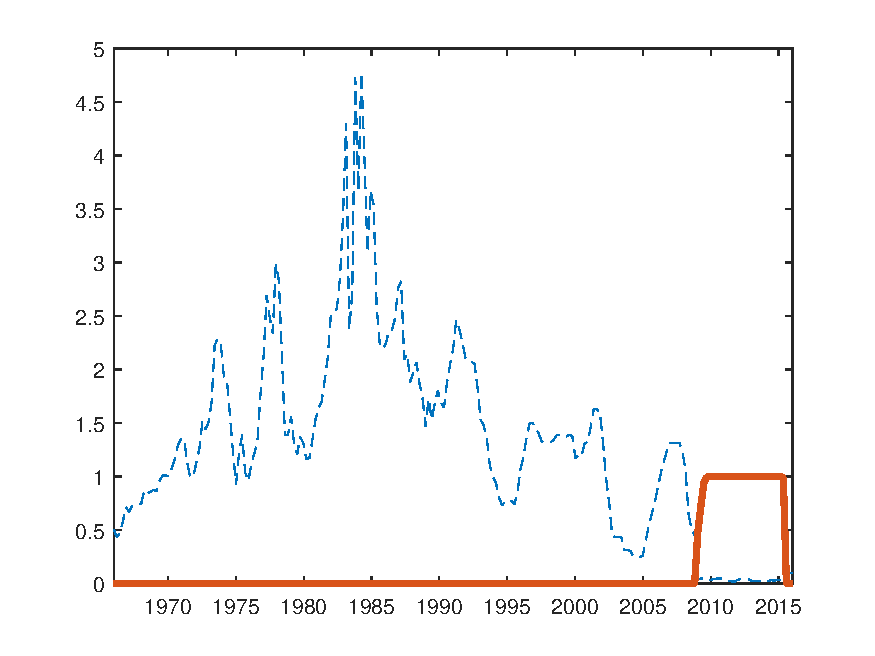
\includegraphics[scale=0.6]{NKPC_ree_init_AR1_regime.pdf} 
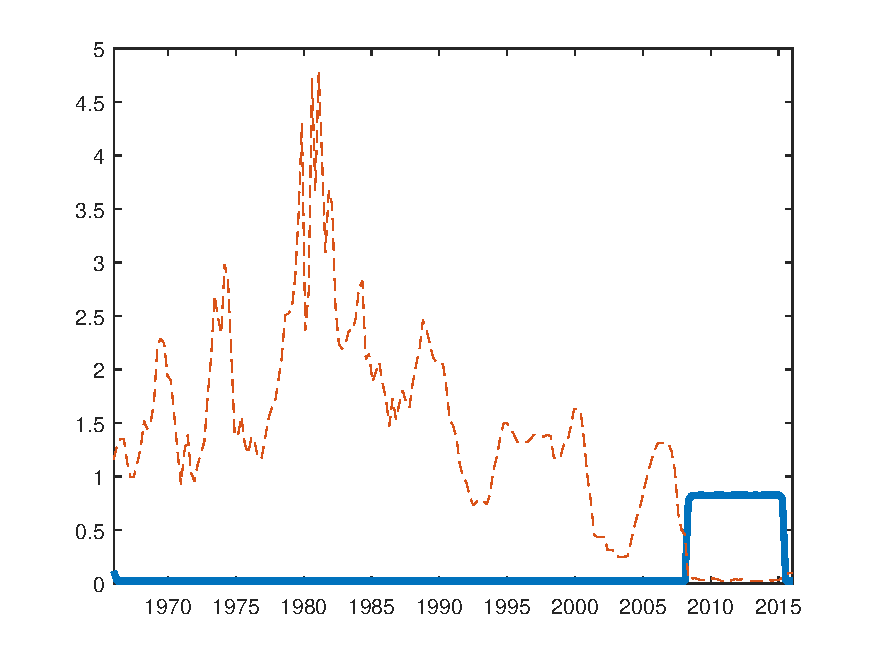
\includegraphics[scale=0.6]{NKPC_sigmaPoint_regime.pdf}\\ 
%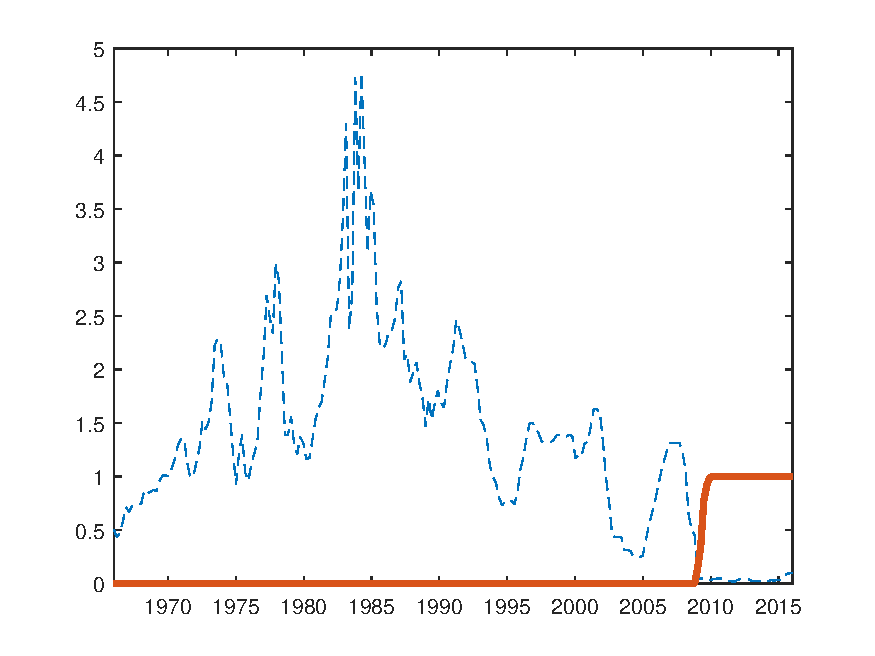
\includegraphics[scale=0.6]{NKPC_ree_init_VAR1_regime.pdf}\\

%\textbf{MSV learning and benchmark MS-REE:}\\

%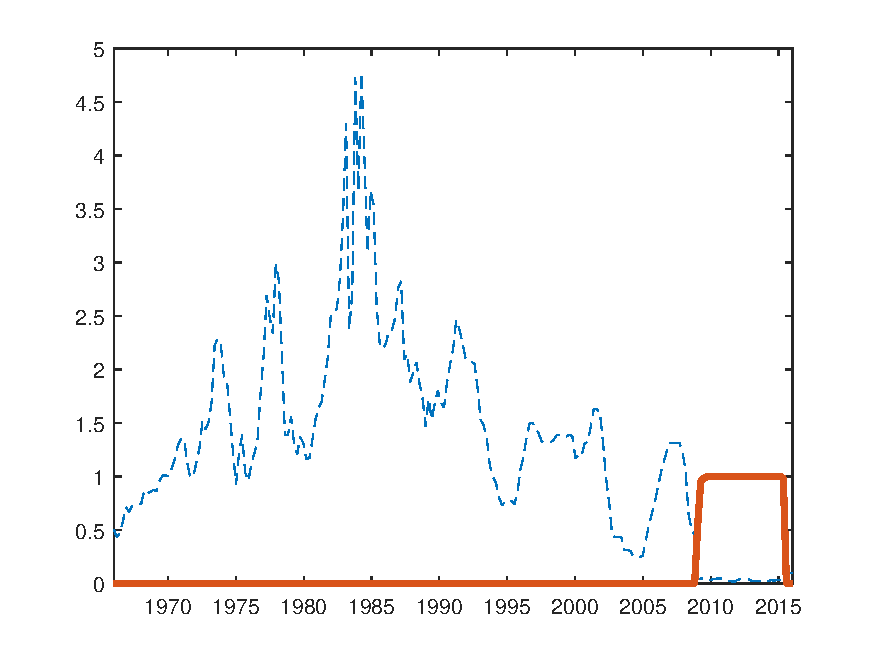
\includegraphics[scale=0.6]{NKPC_ree_init_MSV_regime.pdf}



\end{figure}


\begin{figure}[H]
\label{nkpc_learning_coef}

\caption{Expectation coefficients for AR(1), VAR(1) and MSV-learning cases.}
\vspace{5 mm}
{AR(1) intercept and persistence coefficients, with output gap and inflation on the first and second row respectively.}\\
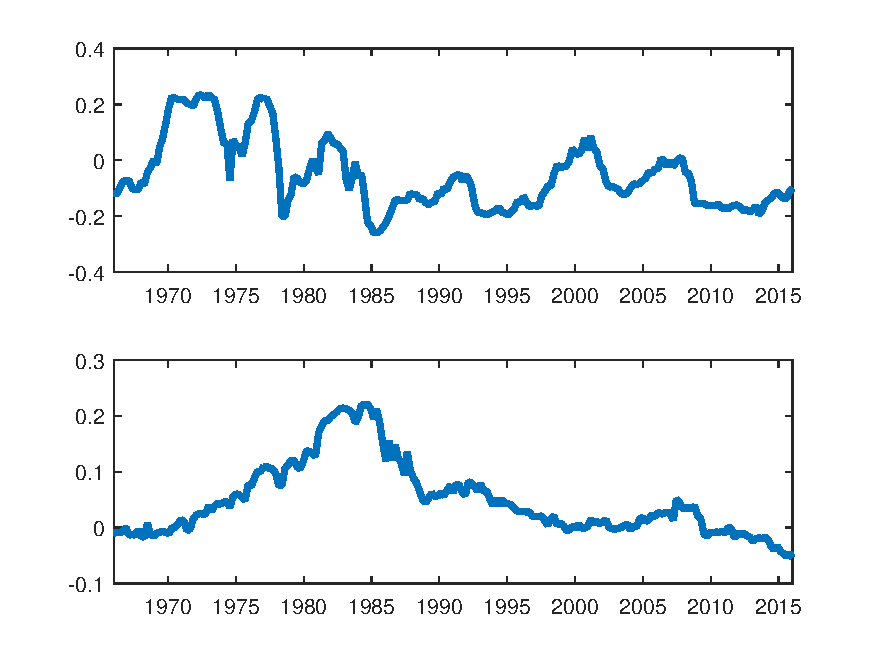
\includegraphics[scale=0.35]{NKPC_ree_init_AR1_alphas.pdf}
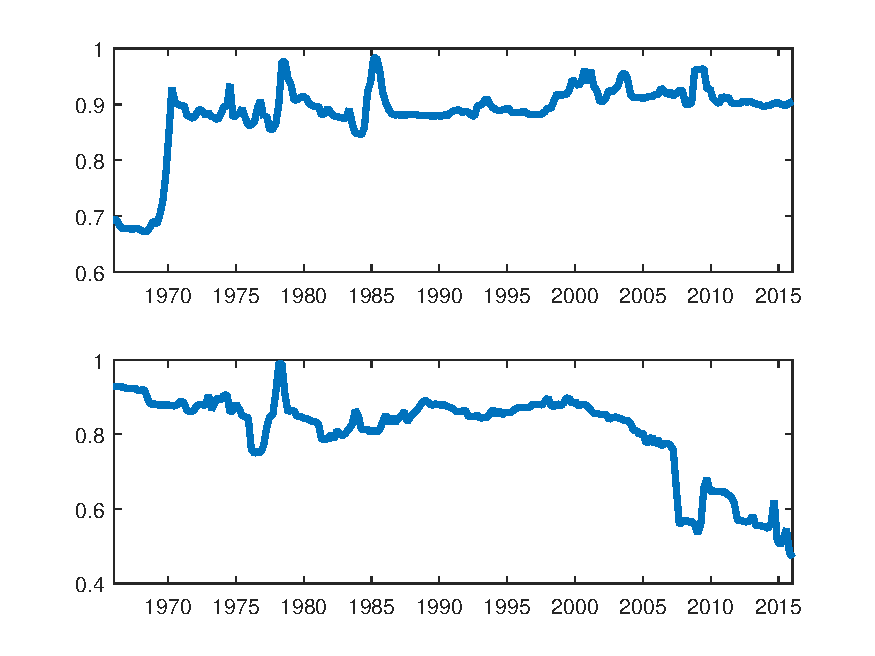
\includegraphics[scale=0.35]{NKPC_ree_init_AR1_betas.pdf}\\

{VAR(1) intercept and  cross-correlation coefficients. The left panel shows the perceived intercepts of output gap, inflation and interest rates respectively. The right panel shows the impact of lagged output gap, inflation and interest rates on the first, second and third rows respectively.  }\\
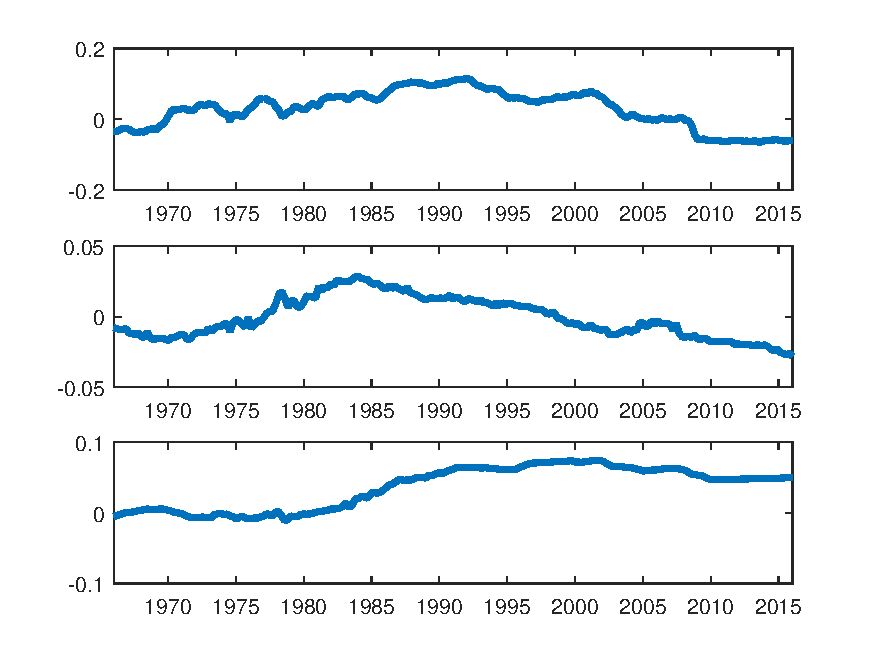
\includegraphics[scale=0.35]{NKPC_ree_init_VAR1_alphas.pdf}
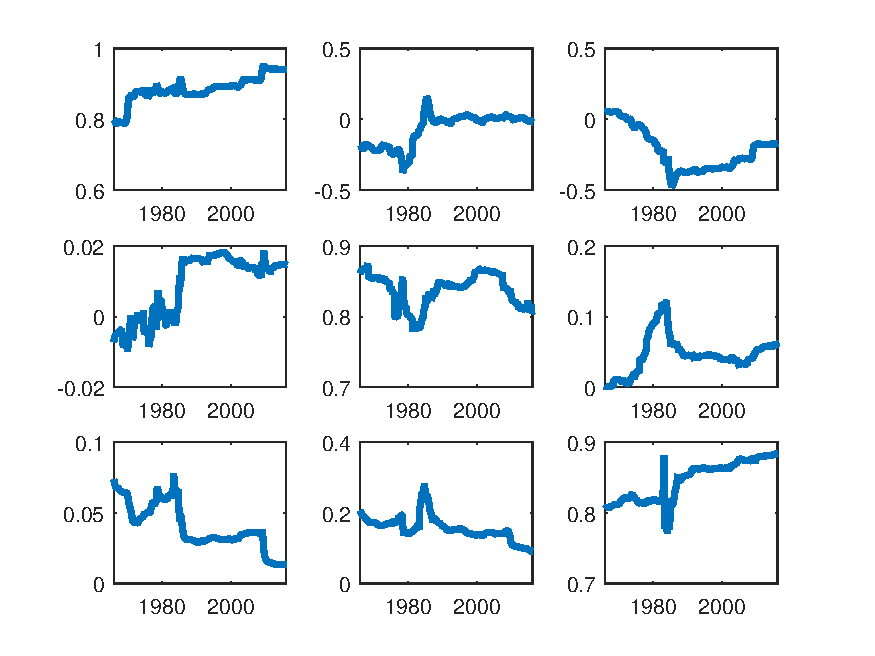
\includegraphics[scale=0.35]{NKPC_ree_init_VAR1_betas.pdf}\\

{MSV learning coefficients. The right panel shows the perceived intercepts of output gap, inflation and interest rates ; the middle panel shows the impact of lagged interest rates on output gap, inflation and interest rates; and the right panel shows feedback coefficients from supply and demand shocks on output gap and inflation respectively. }\\
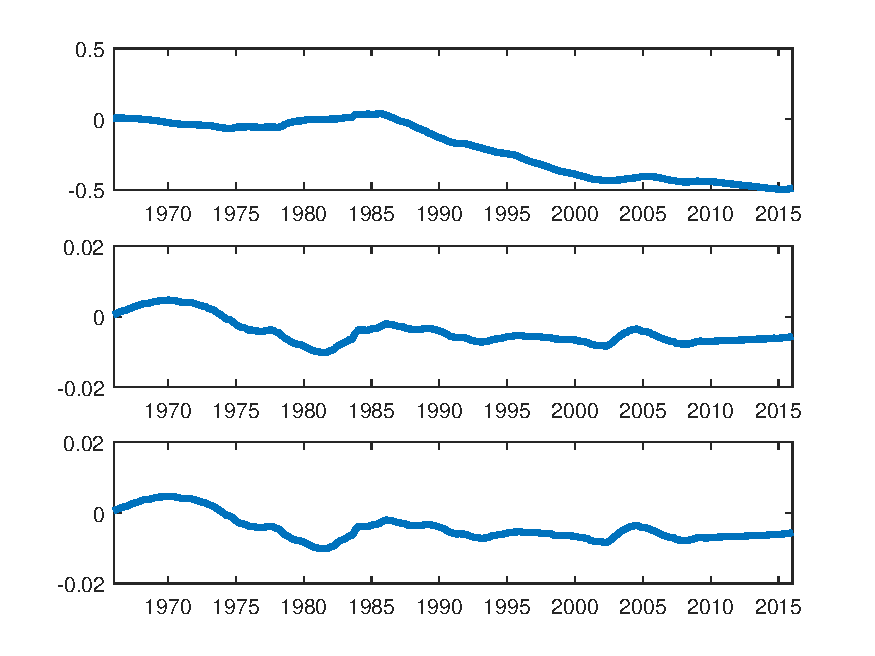
\includegraphics[scale=0.35]{NKPC_ree_init_MSV_alphas.pdf}
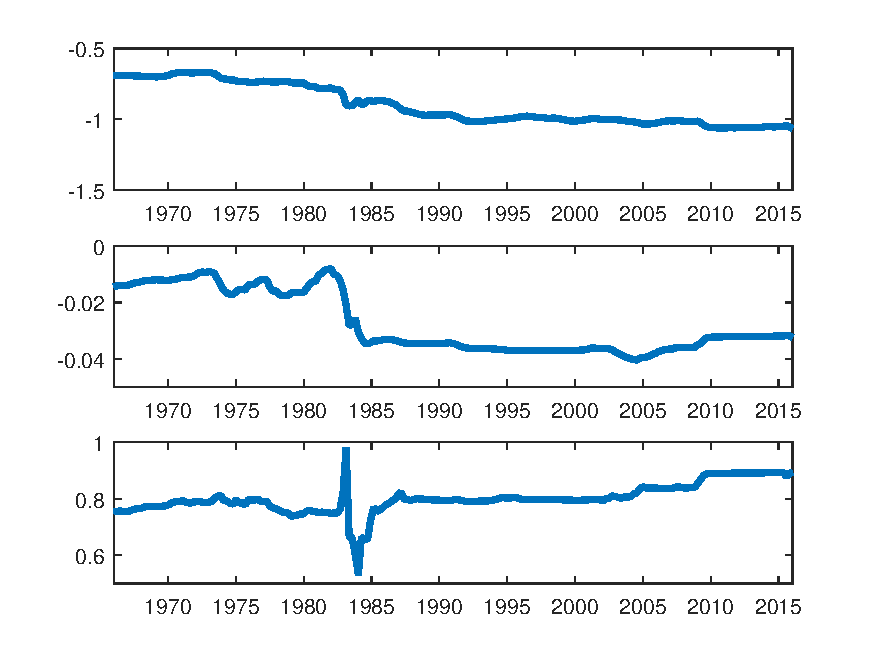
\includegraphics[scale=0.35]{NKPC_ree_init_MSV_betas.pdf}
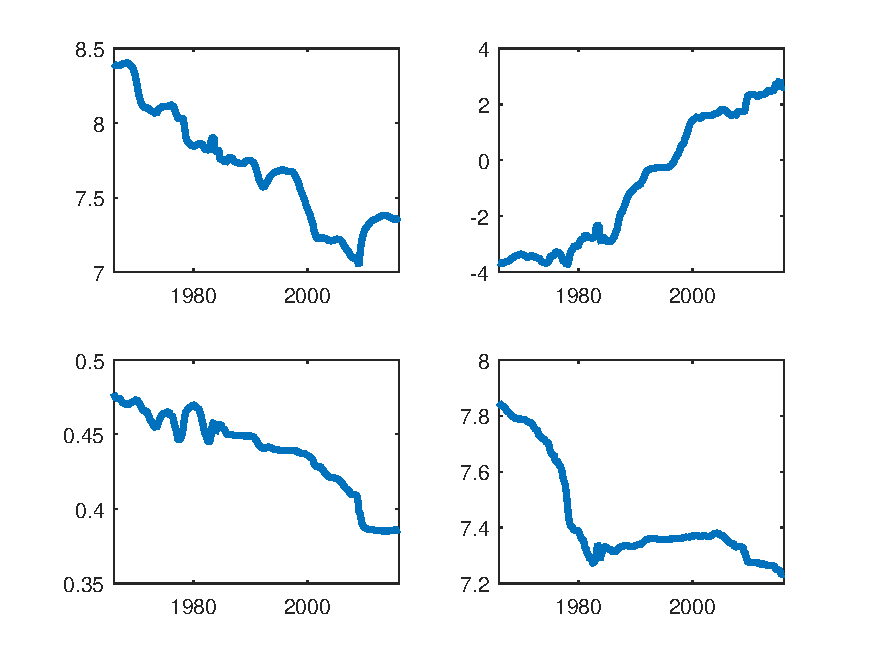
\includegraphics[scale=0.35]{NKPC_ree_init_MSV_shockCoef.pdf}\\

\end{figure}

\begin{figure}[H]
\caption{Impulse responses of time-varying PLMs are based on an arbitrary period.}
\label{nkpc_impulse}
\textbf{AR(1) and VAR(1) beliefs:}\\
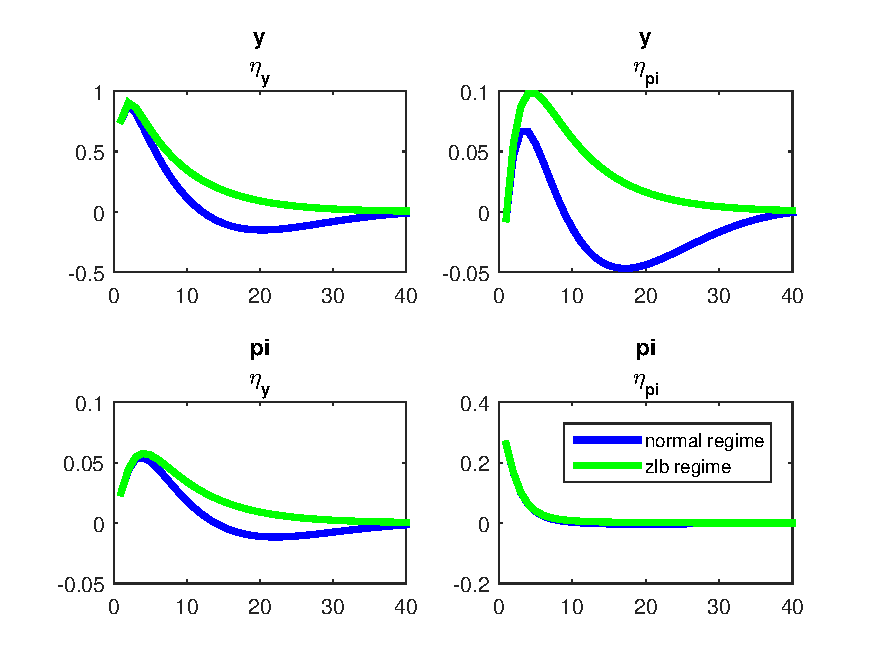
\includegraphics[scale=0.6]{NKPC_ree_init_AR1_IR.pdf}
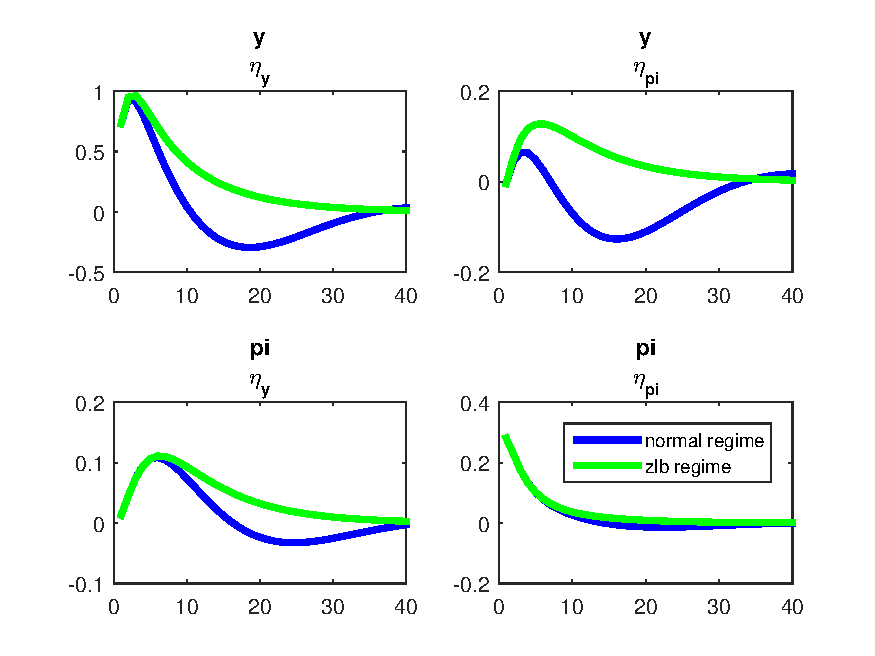
\includegraphics[scale=0.6]{NKPC_ree_init_VAR_IR.pdf}\\

\textbf{MS and standard REE benchmarks: }\\

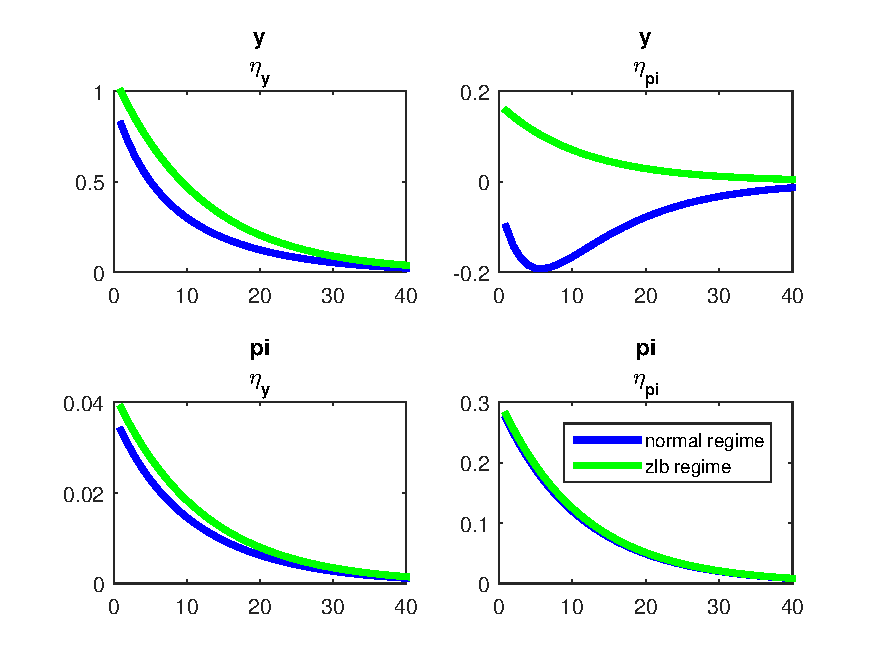
\includegraphics[scale=0.6]{NKPC_ree_init_REE_MS_IR.pdf}
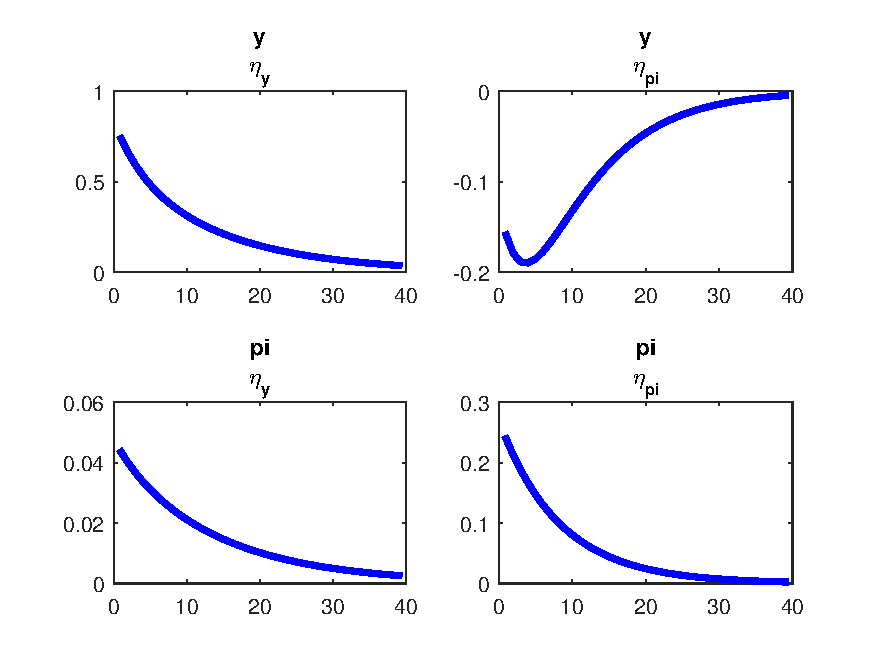
\includegraphics[scale=0.6]{NKPC_ree_init_REE_IR.pdf}\\

\textbf{MSV beliefs: }\\

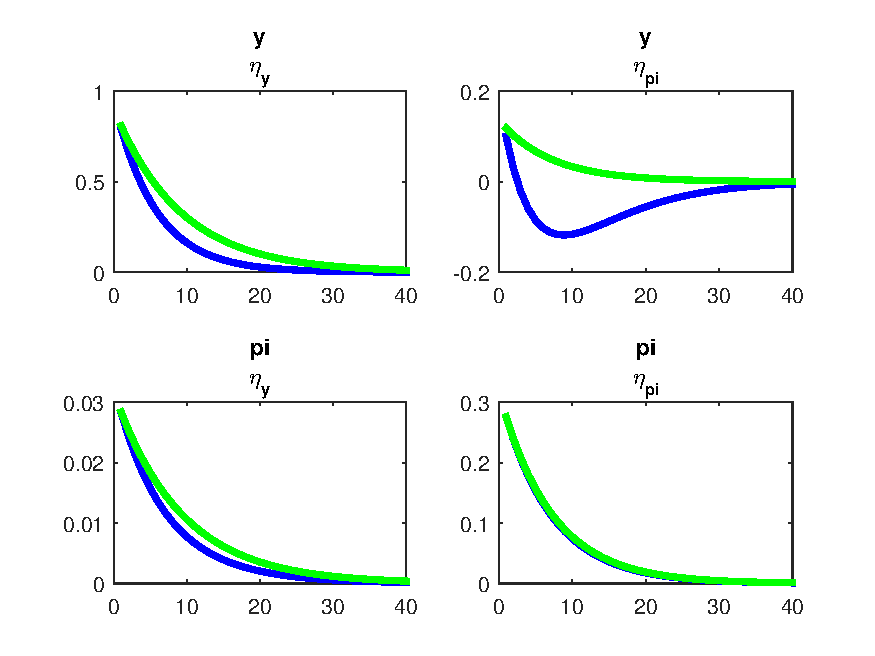
\includegraphics[scale=0.6]{NKPC_ree_init_MSV_IR.pdf}\\





\end{figure}

\section{Estimation of Smets-Wouters}

In this section we consider the estimation of Smets-Wouters (2007). The prior distributions of the benchmark parameters are identical to Smets-Wouters, while the ZLB and learning related parameters are the same as in the 3-equation model above. Accordingly, we have seven structural shocks: productivity, risk-premium, government spending, investment, monetary policy, and 
price \& wage mark-up shocks, denoted by $a$, $b$, $g$, $i$, $r$, $p$ and $w$, see Smets-Wouters (2003, 2007) for more details. Our only deviation from the benchmark model is to assume that the mark-up shocks follow an AR(1) process, instead of the original ARMA(1,1) assumption: as shown in Slobodyan \& Wouters (2012b ??), these shock processes are typically close to being white noise when expectations are assumed to be backward-loooking, in which case the AR(1) and MA(1) terms are close to being locally unidentified. Therefore we assume away the MA(1) terms and model these shocks as AR(1) processes. The rest of the model is left unchanged. Our measurement equations also follow the benchmark case, where we use seven observables as follows:

$$
\begin{cases}
 d( log(y^{obs}_t)) = \bar{\gamma} + (y_t - y_{t-1} ) \\
d(log(c^{obs}_t)) = \bar{\gamma} + (c_t - c_{t-1} )\\
d(log({inv}^{obs}_t)) = \bar{\gamma} + ({inv}_t - inv_{t-1} )\\
d(log(w^{obs}_t)) = \bar{\gamma} + (w_t - w_{t-1} )\\
log(l^{obs}_t) = \bar{l} + l_t\\
(log(\pi^{obs}_t)) = \bar{\pi} + \pi_t \\
(log(r^{obs}_t)) = \bar{r} + r_t\\
\end{cases}
$$

where $ d( log(y^{obs}_t)) $, $ d(log(c^{obs}_t)) $ , $ d(log({inv}^{obs}_t)) $ and $d(log(w^{obs}_t)) $ denote real output, consumption, investment and wage growths with the common growth rate $\bar{\gamma}$ respectively, while $log(l^{obs}_t)$, $(log(\pi^{obs}_t)) $ and $(log(r^{obs}_t)) $ denote (normalized) hours worked, inflation rate and federal funds rate respectively. We use the same estimation sample as in the 3-equation NKPC with quarterly U.S. data covering the period from 1966:I to 2016:IV. 
%In this section we also consider the post-Great Moderation (GM) period of 1985:I-2016:IV as an alternative. Further, since the VAR(1)-learning model yields the same implications as the AR(1)-learning model and has the worst likelihood amont the learning models, we only consider the AR(1)- and MSV-learning cases here.  \ref{sw_estimation_subsample}
 Figure \ref{sw_estimation_full} shows the full sample results for the learning and benchmark REE and MS-REE cases. We observe that our main conclusions from the NKPC-estimation continue to hold in this more realistic setup: the MS-REE model considerably improves upon the REE benchmark with likelihoods -1171 and -1213 respectively, which shows the empirical importance of explicitly modeling the ZLB episode. The MSV-learning setup yields a likelihood of -1168, which is very close to the REE-MS case. This indicates the time-variation under MSV-learning does not lead to any meaningful improvements over the MS-REE model. Next looking at the parsimonious AR(1) learning case, we have a likelihood of -1135, which is another substantial improvement over both the MSV-learning and MS-REE cases. The model with the univariate, backward-looking expectation rule is thus our preferred specification based on thes results. Taken together with the NKPC estimations, all of our results are consistent with the previous literature on learning: Milani (??) shows that MSV-learning performs better that REE in the small 3-equation setup, while Slobodyan \& Wouters (2012a?) find that this result does not extend to the medium-scale setup of SW model, where MSV-learning does not lead to improvements over the REE model. Instead using a univariate backward-looking rule in Slobodyan \& Wouters (2012b?), they find that the model fit improves considerably. Our results in this section and the previous one confirm these results, and show that they continue to hold in a Markov-switching setup where the ZLB episode is considered. \\
\noindent
Next we turn to a discussion of our parameter estimates and we focus particularly on the learning, ZLB and nominal friction parameters. Starting with the estimated exit probabilities from the normal and ZLB regimes, we can see the same result as in the 3-equation model, where the ZLB regime becomes more persistent under the learning cases. In particular, the estimated exit probability from the ZLB regime is 0.29 under the MS-REE model, indicating an expected ZLB duration of of $~3.5$ quarters. This probability is substantially larger under the learning specifications with a value of 0.13 under bothn AR(1) and MSV-learning cases, which suggests an expected ZLB duration of $~7.7$ quarters. Especially the expected duration under the MS-REE case is lower compared to the 3-equation model, suggesting there is downward pressure for the persistence of this regime. It is important to note that the expected ZLB durations both under the MS-REE and learning cases are substantially lower than the empirical length of the ZLB episode, which lasted around 7 years or 28 quarters for the U.S. economy. However, our results suggest that adaptive learning is indeed one way of increasing the expected duration of this episode, since the expected duration in the Smets-Wouters model is estimated more than twice under adaptive learning compared with the MS-REE case. \\
\noindent
The estimated gain values for both AR(1)- and MSV-learning cases are substantially lower compared with the 3-equation model, with values of 0.012 and 0.001 respectively. Branch \& Evans (??) find that values over the range $[0.01,0.05]$ provide a good fit for the Survey of Professional Forecasters (SPF) dataset. Accordingly, the resulting gain value under AR(1)-learning is still in the empirically relevant range, while the under MSV-learning it is significantly closer to zero. This suggests either that the MSV information set is not supported by the data, or that the initial beliefs provide a better fit than the time-variation in beliefs under the MSV-setup. At the estimated value under MSV-learning, the initial beliefs receive a weight of $(1-0.001)^200 \approx 0.82$ at the end of the sample; i.e. beliefs remain very close to the initial beliefs during the entire estimation sample. The resulting likelihoods suggest that this does not lead to substantial differences in the model fit, which is also evident from the remaining parameter estimates. The only exceptions are the price and wage Calvo probabilities, which are slightly lower under the MSV-learning case compared with the MS-REE. The difference is more pronounced under AR(1)-learning, where the Calvo probabilities keep decreasing further. This suggests nominal persistence parameters become less pronounced as expectations become more sluggish, which is also consistent with the findings in previous literature. Another important difference that arises under AR(1)-learning is the shock persistence terms: the price and wage mark-up shocks become near white noise processes with persistence near zero, while the persistence of investment shock also becomes substantially smaller. Finally, the implied consumption dynamics are very different under AR(1) learning: both the capital adjustment cost $\phi$ and habit formation $\lambda$ parameters are lower compared to the remaining cases, while the inverse intertemporal elasticity of substitution decreases to below one. An interesting implication of this is that, under AR(1) learning, consumption and labor become substitutes rather than complements. \\
\noindent
Overall, our results suggest that the univariate AR(1)-learning case provides the best model fit and leads to some important differences in the model structure as a whole, while the MSV-learning remains very close to the MS-REE model. In both cases, however, there is a sizeable increase in expected duration of the ZLB episode, which brings the persistence of this regime closer to the empirically relevant region. \\
\noindent



\begin{table}[H]
\caption{Estimation period: 1966:I-2016:IV}
\label{sw_estimation_full}
\begin{tabular}{llll|ll|lll}
 & Prior &  &  & AR(1) & MSV & REE & MS-REE &  \\
 \hline
 \hline
Param &  & Dist & Mean & Mode & Mode & Mode & Mode &  \\
\hline
\hline
$\phi$ &  & Normal & 4        		& 1.02 & 3.75 & 4.87 & 6.4 \\
$\sigma_c$ &  & Normal & 1.5		& 0.88 & 1.48 & 1.36 & 1.14 \\
$\lambda$ &  & Beta & 0.7 			& 0.55 & 0.73 & 0.75 & 0.83 \\
$\xi_w$ &  & Beta & 0.5 			& 0.7 & 0.75 & 0.93 & 0.95 \\
$\sigma_l$ &  & Normal & 2 			& 2.41 & 2.18 & 1.98 & 1.74 \\
$\xi_p$ &  & Beta & 0.5 			& 0.62 & 0.67 & 0.8 & 0.83 \\
$\iota_w$ &  & Beta & 0.5 			& 0.43 & 0.63 & 0.84 & 0.81 \\
$\iota_p$ &  & Beta & 0.5 			& 0.40 & 0.23 & 0.07 & 0.08 \\
$\psi$ &  & Beta & 0.5 				& 0.49 & 0.69 & 0.83 & 0.69 \\
$\phi_p$ &  & Normal & 1.25 		& 1.49 & 1.57 & 1.59 & 1.56 \\
$r_{\pi}$ &  & Normal & 1.25 		& 1.64 & 1.62 & 1.5 & 1.35 \\
$\rho$ &  & Beta & 0.75 			& 0.88 & 0.88 & 0.85 & 0.86 \\
$r_y$ &  & Normal & 0.125 			& 0.13 & 0.12 & 0.05 & 0.06 \\
$r_{dy}$ &  & Normal & 0.125 		& 0.14 & 0.14 & 0.17 & 0.19 \\
$\bar{\pi}$ &  & Gamma & 0.625 		& 0.71 & 0.86 & 0.75 & 0.76 \\
$\bar{\beta}$ &  & Gamma & 0.25 	& 0.14 & 0.19 & 0.21 & 0.25 \\
$\bar{l}$ &  & Normal & 0 			& 0.73 & 1.59 & -1.2 & 0.15 \\
$\bar{\gamma}$ &  & Normal & 0.4 	& 0.4 & 0.43 & 0.4 & 0.41 \\
$\alpha$ &  & Normal & 0.3 			& 0.15 & 0.16 & 0.17 & 0.18 \\
$\rho_a$ &  & Beta & 0.5 			& 0.98 & 0.95 & 0.96 & 0.95 \\
$\rho_b$ &  & Beta & 0.5 			& 0.35 & 0.42 & 0.36 & 0.29 \\
$\rho_g$ &  & Beta & 0.5 			& 0.99 & 0.99 & 0.98 & 0.98 \\
$\rho_i$ &  & Beta & 0.5 			& 0.48 & 0.83 & 0.83 & 0.76 \\
$\rho_r$ &  & Beta & 0.5 			& 0.15 & 0.07 & 0.08 & 0.16 \\
$\rho_p$ &  & Beta & 0.5 			& 0.03 & 0.64 & 0.81 & 0.78 \\
$\rho_w$ &  & Beta & 0.5 			& 0.04 & 0.19 & 0.06 & 0.05 \\
$\rho_{ga}$ &  & Beta & 0.5 		& 0.52 & 0.5 & 0.53 & 0.51 \\
$\eta_a$ &  & Inv. Gamma & 0.1 		& 0.46 & 0.43 & 0.44 & 0.45 \\
$\eta_b$ &  & Inv. Gamma & 0.1 		& 0.68 & 0.21 & 0.21 & 0.23 \\
$\eta_g$ &  & Inv. Gamma & 0.1 		& 0.48 & 0.48 & 0.49 & 0.48 \\
$\eta_i$ &  & Inv. Gamma & 0.1 		& 1.36 & 0.36 & 0.36 & 0.34 \\
$\eta_{r,N}$ &  & Inv. Gamma & 0.1 	& 0.21 & 0.21 & 0.21 & 0.23 \\
$\eta_{r,ZLB}$ &  & Gamma & 0.03 	& 0.01 & 0.01 & - & 0.01 \\
$\eta_p$ &  & Inv. Gamma & 0.1 		& 0.27 & 0.07 & 0.05 & 0.06 \\
$\eta_w$ &  & Inv. Gamma & 0.1 		& 0.73 & 0.35 & 0.37 & 0.37 \\
$gain$ &  & Gamma & 0.035 			& 0.012 & 0.001 & - &  -\\
$1-p_{11}$ &  & Beta & 0.1 			& 0.02 & 0.02 & - & 0.01 \\
$1-p_{22}$ &  & Beta & 0.1 			& 0.13 & 0.13 & - & 0.29 \\
$\bar{r_{zlb}}$ &  & Normal & 0.05 	& 0.03 & 0.03 & - & 0.03 \\
 &  &  &  &  &  &  &  \\
Laplace &  &  &  & -1135 & -1168 & -1213 & -1171
\end{tabular}
\end{table}

\begin{comment}

\subsection*{SW Estimations-II}

\begin{table}[H]
\caption{Estimation period: 1985:I-2016:IV}
\label{sw_estimation_subsample}
\begin{tabular}{llll|ll|lll}
 & Prior &  &  & AR(1) & MSV & REE & MS-REE &  \\
 \hline
 \hline
Param &  & Dist & Mean & Mode & Mode & Mode & Mode &  \\
\hline
\hline
$\phi$ &  & Normal & 4 			& 0.86 & 5 & 6.72 & 4.91 &  \\
$\sigma_c$ &  & Normal & 1.5 	& 0.35 & 0.82 & 1.93 & 1.12 &  \\
$\lambda$ &  & Beta & 0.7 		& 0.6 & 0.82 & 0.7 & 0.55 &  \\
$\xi_w$ &  & Beta & 0.5 		& 0.63 & 0.69 & 0.8 & 0.84 &  \\
$\sigma_l$ &  & Normal & 2 		& 2.14 & 2.52 & 1.08 & 1.65 &  \\
$\xi_p$ &  & Beta & 0.5 		& 0.77 & 0.76 & 0.83 & 0.92 &  \\
$\iota_w$ &  & Beta & 0.5 		& 0.48 & 0.59 & 0.5 & 0.46 &  \\
$\iota_p$ &  & Beta & 0.5 		& 0.27 & 0.42 & 0.13 & 0.19 &  \\
$\psi$ &  & Beta & 0.5 			& 0.66 & 0.82 & 0.88 & 0.8 &  \\
$\phi_p$ &  & Normal & 1.25 	& 1.31 & 1.48 & 1.51 & 1.4 &  \\
$r_{\pi}$ &  & Normal & 1.25 	& 1.42 & 1.49 & 1.63 & 1.48 &  \\
$\rho$ &  & Beta & 0.75 		& 0.91 & 0.9 & 0.87 & 0.86 &  \\
$r_y$ &  & Normal & 0.125 		& 0.17 & 0.07 & 0.07 & 0.24 &  \\
$r_{dy}$ &  & Normal & 0.125 	& 0.11 & 0.07 & 0.07 & 0.09 &  \\
$\bar{\pi}$ &  & Gamma & 0.625 	& 0.68 & 0.61 & 0.67 & 0.61 &  \\
$\bar{\beta}$ &  & Gamma & 0.25 & 0.2 & 0.27 & 0.21 & 0.25 &  \\
$\bar{l}$ &  & Normal & 0 		& 3.03 & 5.69 & 1.24 & 3.82 &  \\
$\bar{\gamma}$ &  & Normal & 0.4& 0.45	 & 0.5 & 0.34 & 0.47 &  \\
$\alpha$ &  & Normal & 0.3 		& 0.11 & 0.15 & 0.17 & 0.15 &  \\
$\rho_a$ &  & Beta & 0.5 		& 0.99 & 0.99 & 0.99 & 0.98 &  \\
$\rho_b$ &  & Beta & 0.5 		& 0.60 & 0.58 & 0.34 & 0.96 &  \\
$\rho_g$ &  & Beta & 0.5 		& 0.99 & 0.99 & 0.95 & 0.98 &  \\
$\rho_i$ &  & Beta & 0.5 		& 0.40 & 0.79 & 0.85 & 0.73 &  \\
$\rho_r$ &  & Beta & 0.5 		& 0.66 & 0.52 & 0.46 & 0.48 &  \\
$\rho_p$ &  & Beta & 0.5 		& 0.03 & 0.61 & 0.55 & 0.34 &  \\
$\rho_w$ &  & Beta & 0.5 		& 0.07 & 0.19 & 0.09 & 0.09 &  \\
$\rho_{ga}$ &  & Beta & 0.5 	& 0.39 & 0.4 & 0.45 & 0.4 &  \\
$\eta_a$ &  & Inv. Gamma & 0.1 	& 0.4 & 0.38 & 0.39 & 0.05 &  \\
$\eta_b$ &  & Inv. Gamma & 0.1 	& 0.8 & 0.16 & 0.17 & 0.37 &  \\
$\eta_g$ &  & Inv. Gamma & 0.1 			& 0.38 & 0.39 & 0.4 & 0.3 &  \\
$\eta_i$ &  & Inv. Gamma & 0.1 			& 1.15 & 0.31 & 0.29 & 0.09 &  \\
$\eta_{r,N}$ &  & Inv. Gamma & 0.1 		& 0.09 & 0.08 & 0.08 & 0.09 &  \\
$\eta_{r,ZLB}$ &  & Gamma & 0.03 		& 0.01 & 0.01 & - & - &  \\
$\eta_p$ &  & Inv. Gamma & 0.1			& 0.18 & 0.07 & 0.08 & 0.11 &  \\
$\eta_w$ &  & Inv. Gamma & 0.1 			& 0.86 & 0.4 & 0.43 & 0.42 &  \\
$gain$ &  & Gamma & 0.035 				& 0.013 & 0.008 & - & - &  \\
$1-p_{11}$ &  & Beta & 0.1 				& 0.03 & 0.03 &-  & 0.01 &  \\
$1-p_{22}$ &  & Beta & 0.1 				& 0.13 & 0.13 & - & 0.28 &  \\
$\bar{r_{zlb}}$ &  & Normal & 0.05 		& 0.04 & 0.03 & - & - & - \\
 &  &  &  &  &  &  &  &  \\
Laplace &  &  &  & -515 & -566 & -583 & -552 & 
\end{tabular}
\end{table}

\end{comment}


We next turn to the estimated regime probabilities and activity of projection facilities over the estimation sample for the learning models, which is shown in Figure \ref{sw_regime_prob}: similar to the 3-equation model, in both AR(1)- and MSV-learning cases, we observe a sharp switch to the ZLB regime in the beginning of 2009 where the interest rates drop to near-zero levels, while the economy exits from the ZLB regime towards the end of 2016. The same pattern is also observed in the MS-REE model, which is omitted here. An important difference between the SW model here and the 3-equation model is the projection, which was irrelevant in the small model because it remains stable throughout the estimation sample and as a consequence, the projection facility is never imposed. In the larger SW-model, however, the model is occasionally driven into unstable regions, thereby activating the projection facility. This is shown in the second row of the same figure. The right panel shows the regime-specific and weighted-average (based on the ergodic distribution) eigenvalues along with the activity of projection facility for the MSV-learning case. It is readily seen that, although the ZLB regime is closer to the instability region compared to the normal regime, neither regime becomes unstable in this case and the projection facility is not activated. This is partially due to the fact that the information set under MSV-learning does not affect the autocorrelation structure as much; and partially due to the small gain coefficient under this specification. The left panel shows the same figures for the AR(1)-learning case: in this case, we observe that projection facility is activated twice: the first time is during the beginning of 2000s, and the second time is after the crisis period in 2009. An important observation is that, the ZLB-regime is unstable for extended periods of time, especially during the period from 1990 to 2010. For this case, \textit{how} the projection facility is imposed plays a key role in the system dynamics: recall from the previous section that we only impose the projection facility when the underlying ergodic distribution becomes unstable, while the regime-specific models are allowed to be unstable. In this case, although the ZLB-regime is unstable for long periods, the normal regime is sufficiently stable most of the time such that the projection facility is only activated a couple of times. This way of imposing the projection facility is justified on the grounds of our RPE concept, where the regime-specific models can become temporariliy explosive as long as the underlying ergodic distribution is stable; we are able to keep the activity of projection facility to a minimum based on this notion. \\
\noindent
Next we examine how the learning coefficients evolve over the estimation sample, which are shown in Figures \ref{sw_learning_1} and \ref{sw_learning_2}. In the MSV-learning case, there are 15 variables in the information set of the agent, with the intercept, 7 exogenous shocks and 7 endogenous backward-looking variables. Therefore we only provide the plots and discussion of two of these variables for exposition, but similar arguments can be extended to all variables in the information set. Figure \ref{sw_learning_1} shows the intercept coefficients under both learning cases: the first panel shows the AR(1) while the second one is MSV-learning. As one might expect, the time-variation under MSV-learning is relatively small, where all coefficients remain close to zero and there are no observable jumps. This confirms our conclusion from the previous section that, when shocks are assumed to be observable, the intercept terms receive much less weight in forming expectations. On the contrary with the AR(1) case, we observe much more interesting dynamics: since shocks are unobserved in this case, the intercept terms play an important role in agents’ expectations. A particularly interesting case is the financial crisis period, where we observe an almost uniform reduction in all coefficients. Particularly the coefficients on investment and real value of capital (denoted by $i$ and $q$) respectively) decrease by a relatively large amount, while remaining coefficients decrease moderately. This implies that, under AR(1)-learning with unobserved shocks, the crisis and subsequent \textit{Great Recession} period is interpreted as a level shift in the variables by agents, as opposed to a series of adverse shocks. Figure \ref{sw_learning_2} shows the learning coefficients on persistence for the AR(1) case, and lagged inflation for the MSV-learning case. The same results applies to the MSV-learning again, where we do not observe any meaningful time-variation in the coefficients, especially during the crisis period. While we omit the remaining coefficients for the MSV case on lagged variables and exogenous shocks, similar patterns can be observed for these cases as well. Next looking at the AR(1) case which is shown in the first panel, we can again observe a jump in the coeficients during the crisis period, where some of the persistence parameters temporariliy go above one. In other words, when the crisis hits and the agents observe the large downward movement in the endogenous variables, they compensate for this by temporarily switching from a trend-following rule to an extrapolative one. This can be interpreted as a temporary wave of pessimism in the economy, where the agents expect more downward movement following the adverse shock after the crisis. \\

-forecast errors\\
-impulse responses: focus on government spending and risk premium shocks\\
-comment on time-varying plots\\


\begin{figure}[H]
\label{sw_regime_prob}
\caption{Estimated regime probabilities and projection facility in AR(1)- and MSV-learning cases.} 
\vspace{5 mm}
\textbf{Filtered ZLB regime probability:}\\

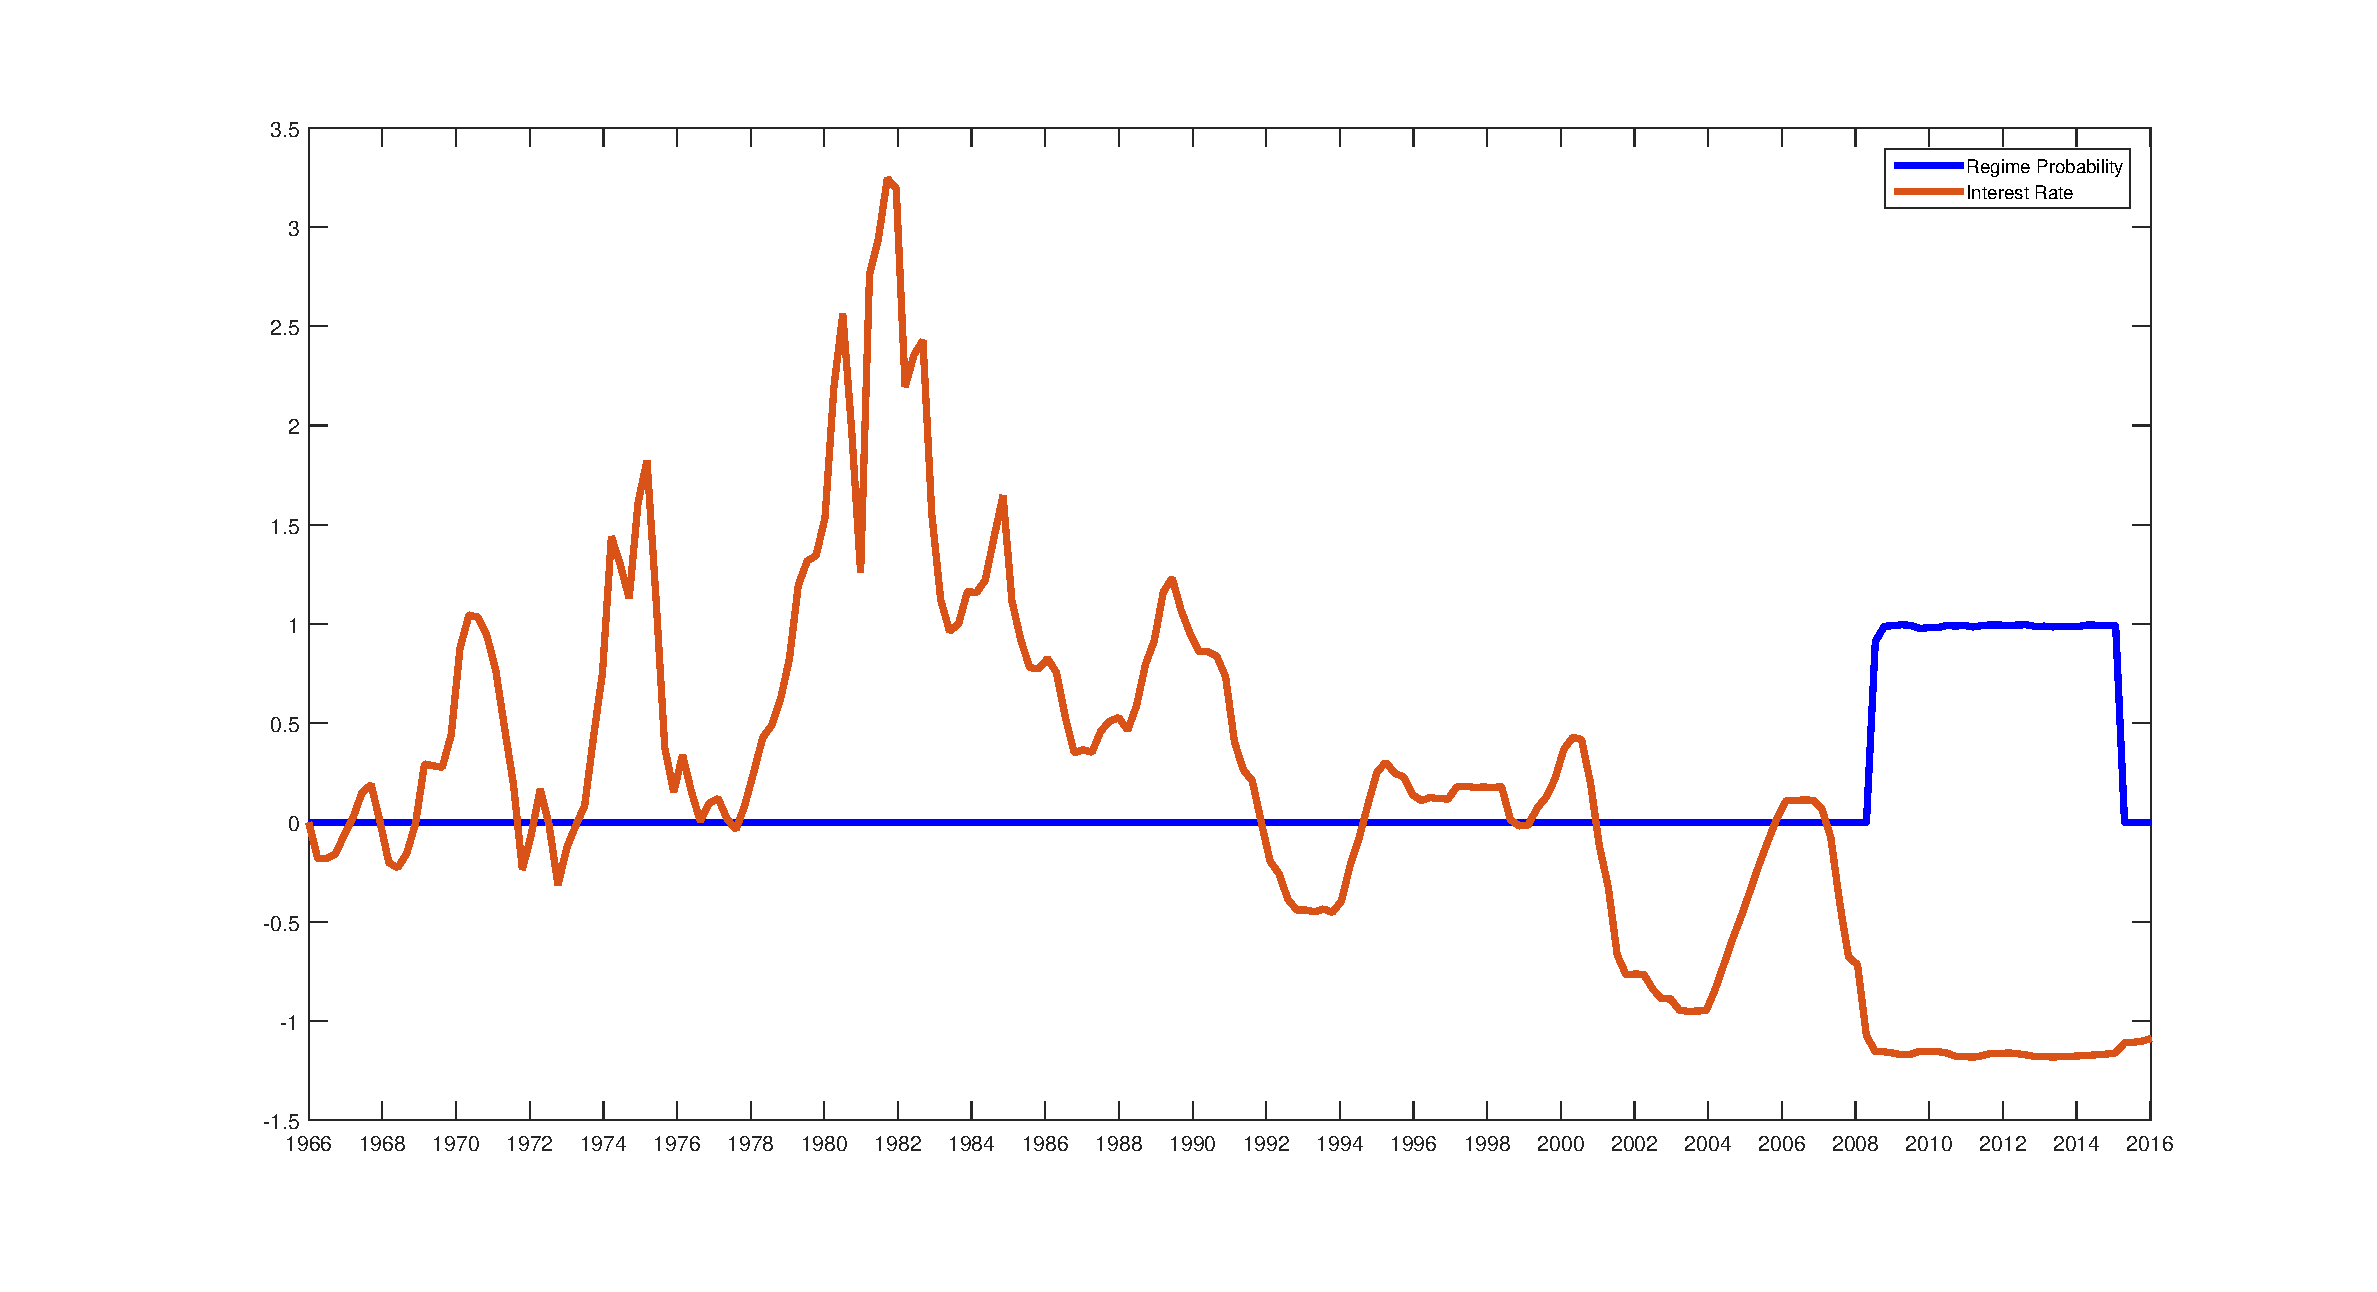
\includegraphics[scale=0.23]{sw_ar1_regimeProb.pdf}
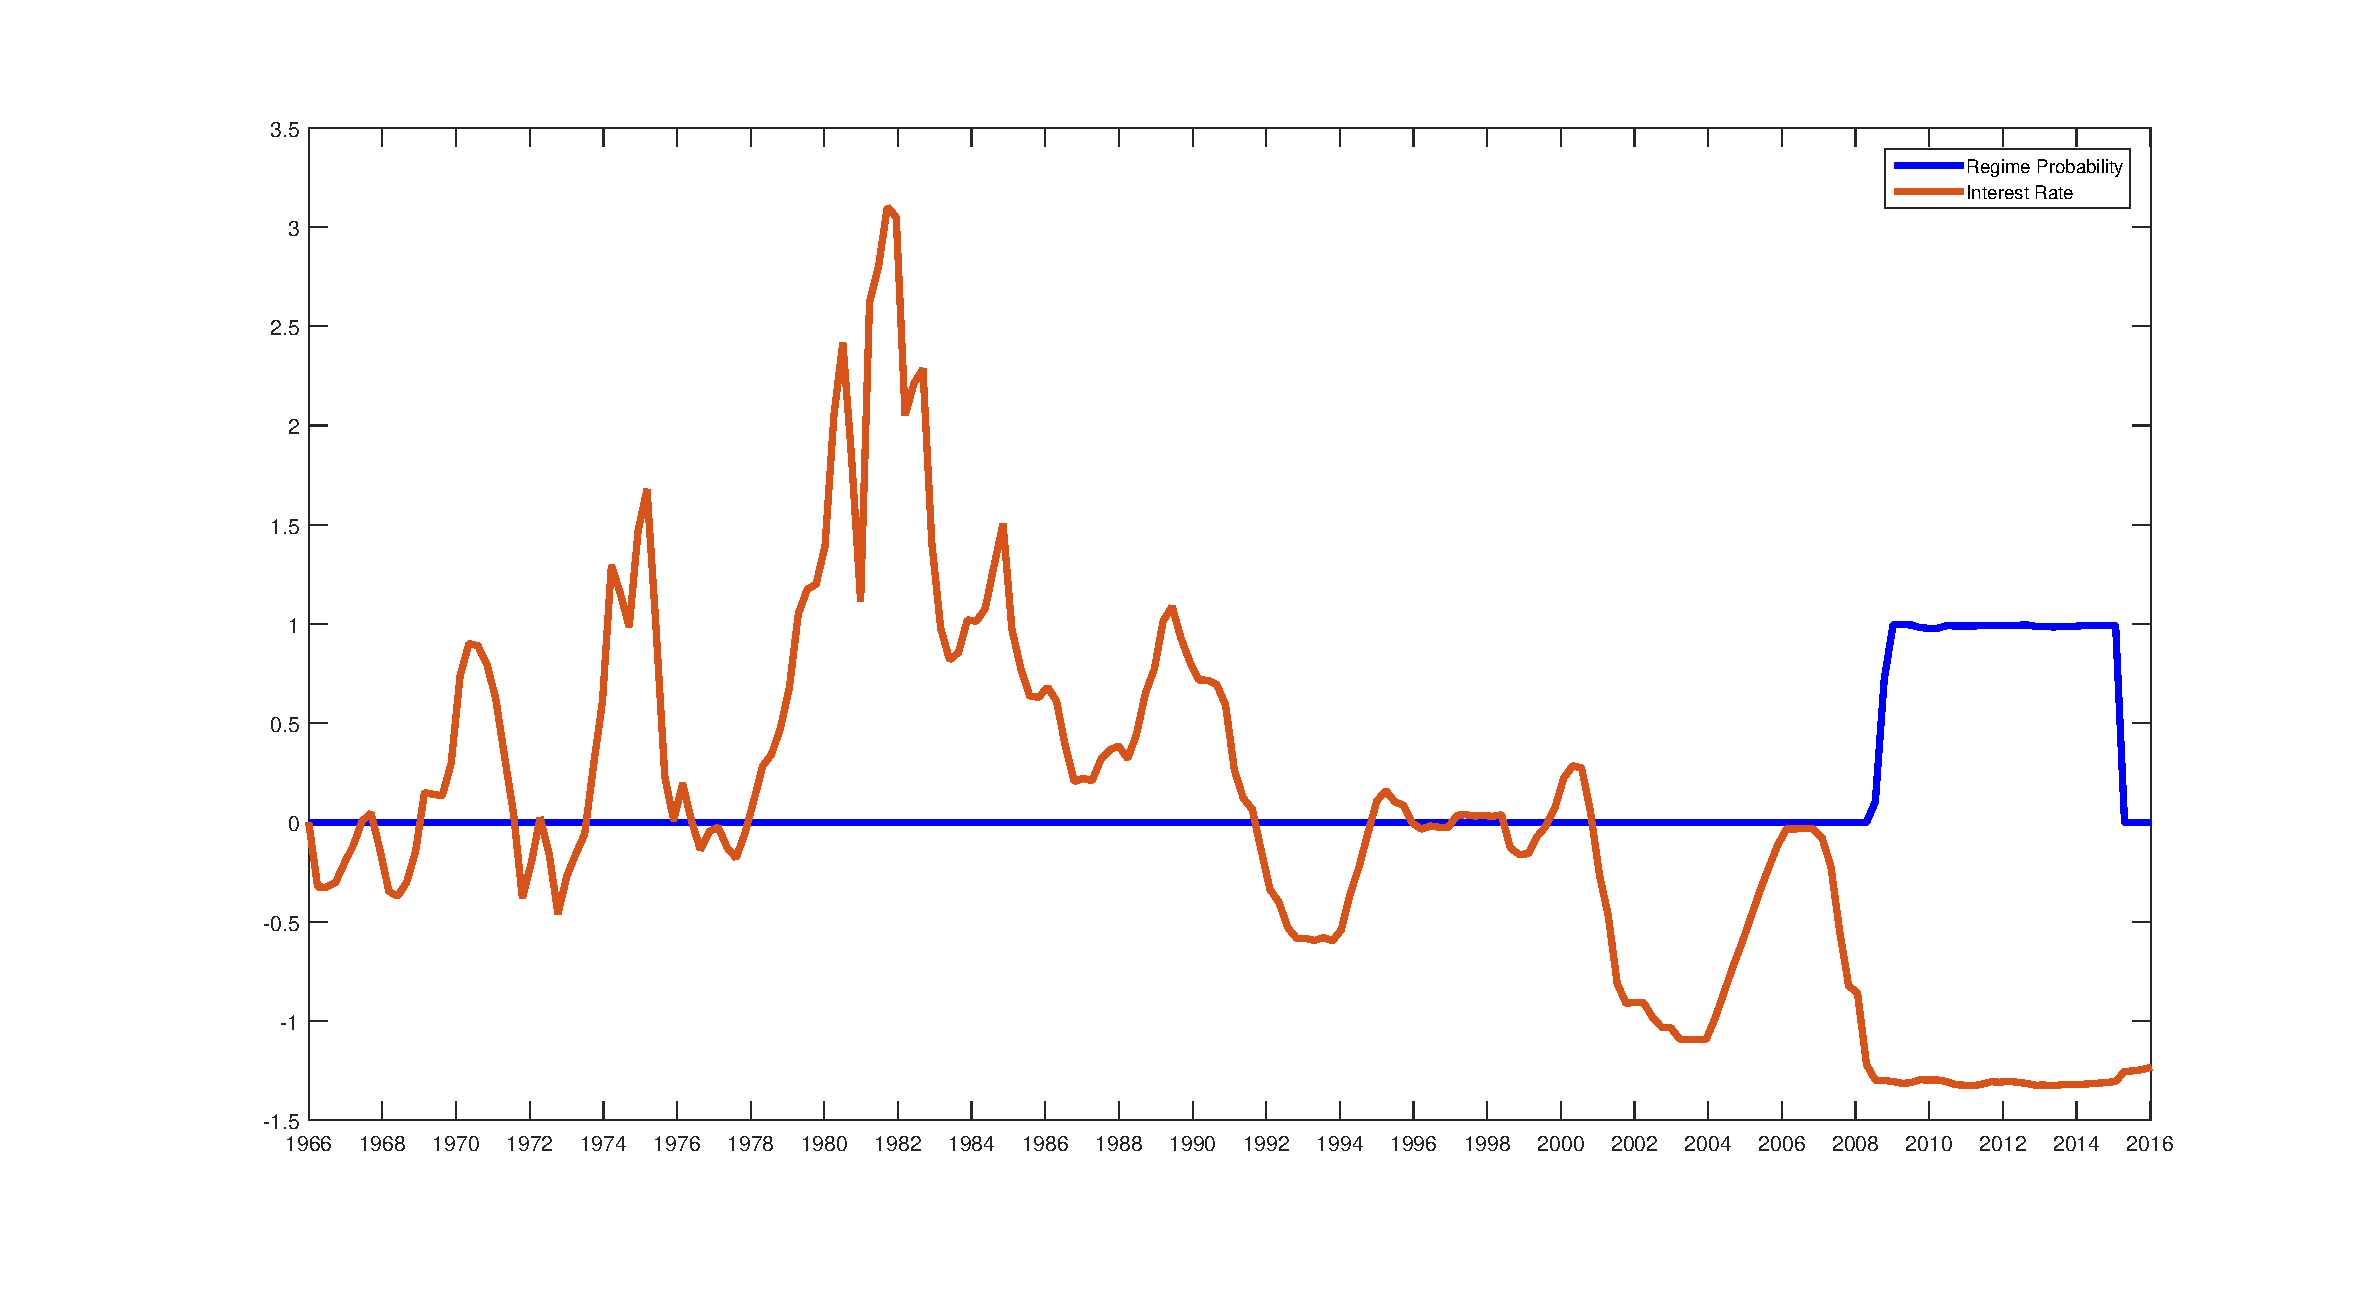
\includegraphics[scale=0.23]{sw_msv_regimeProb.pdf}\\

\textbf{Eigenvalues and Projection Facilities:}\\

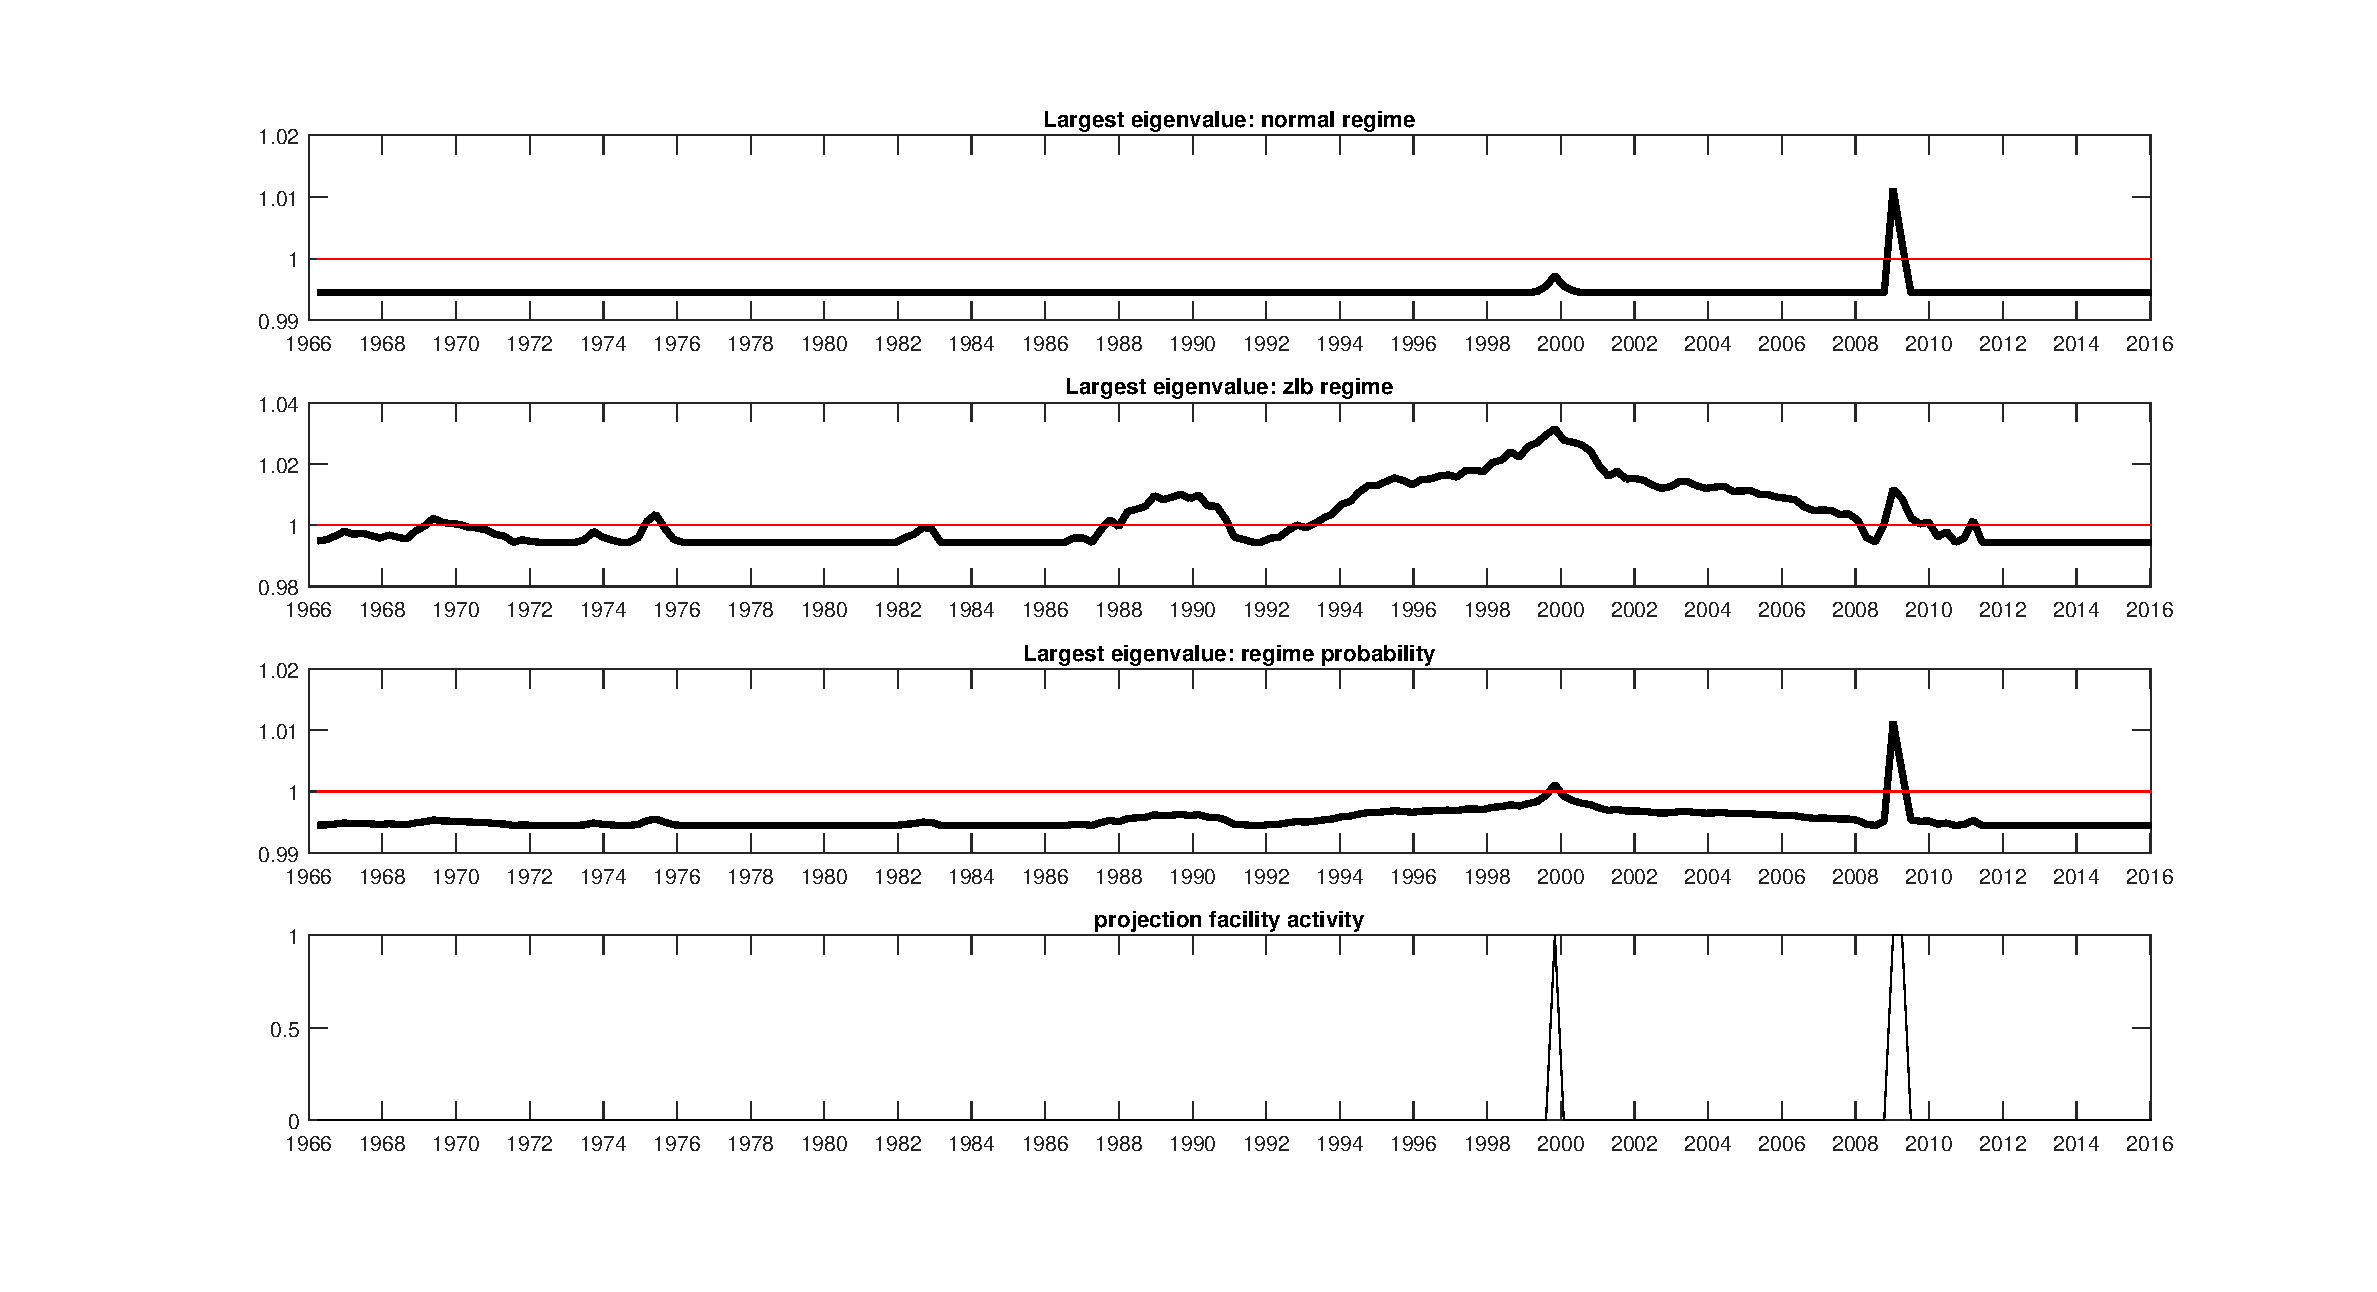
\includegraphics[scale=0.23]{sw_ar1_eigenvalues.pdf}
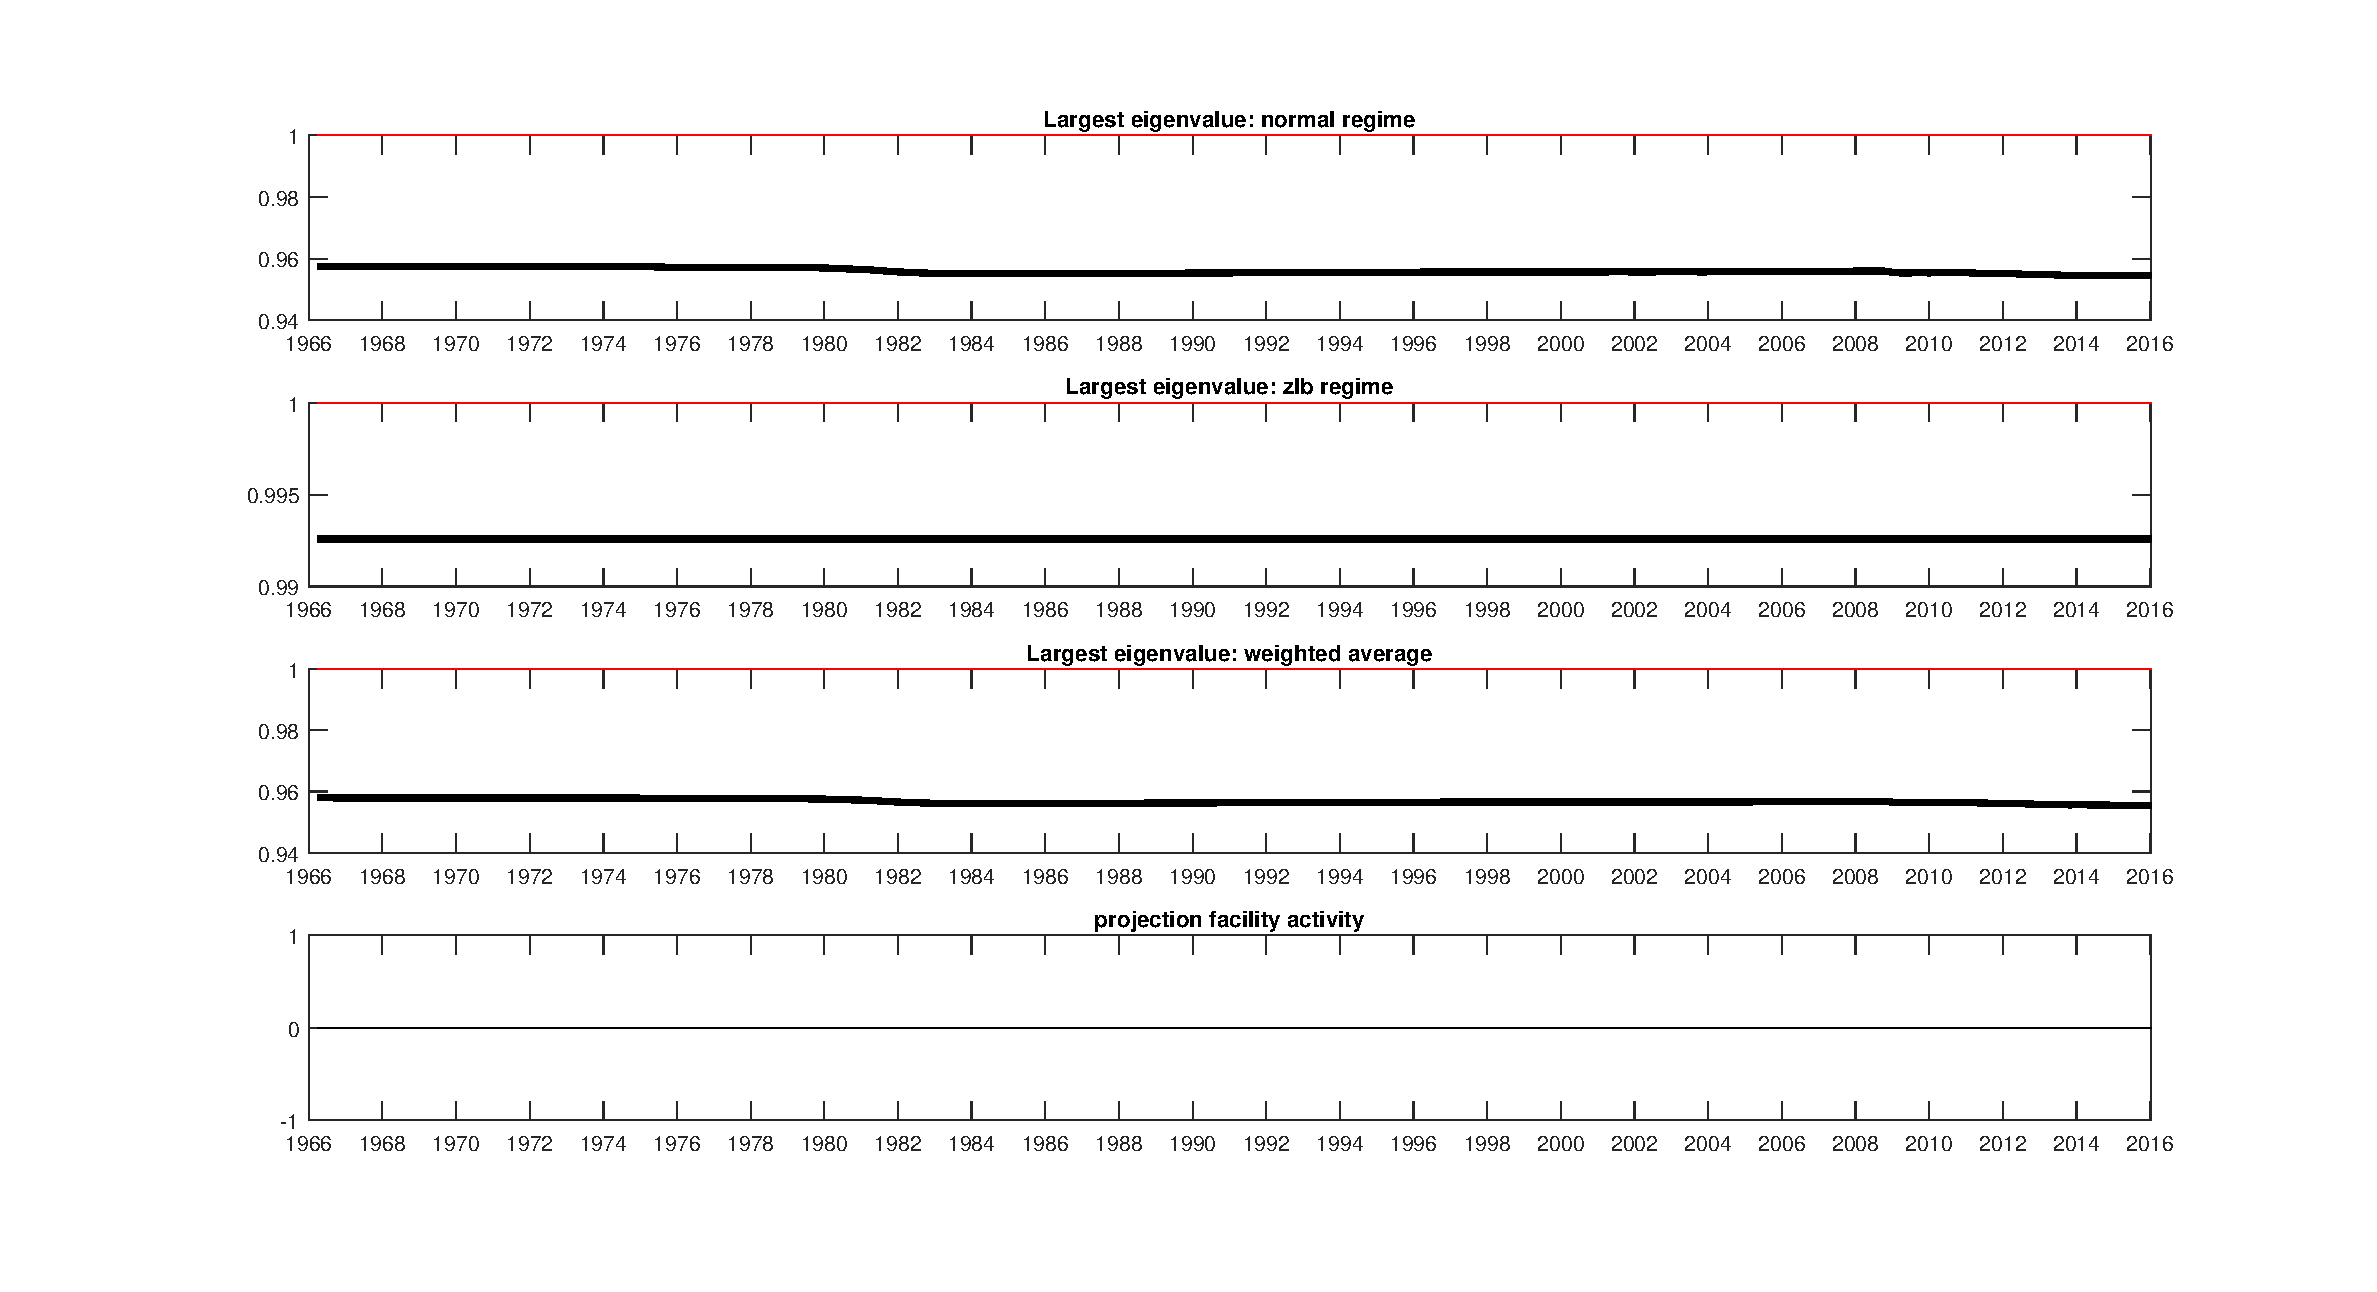
\includegraphics[scale=0.23]{sw_msv_eigenvalues.pdf}
\end{figure}

\begin{figure}[H]
\label{sw_learning_1}
\caption{Learning coefficients in the AR(1)- and MSV-learning cases: Intercepts.} 
\vspace{5 mm}

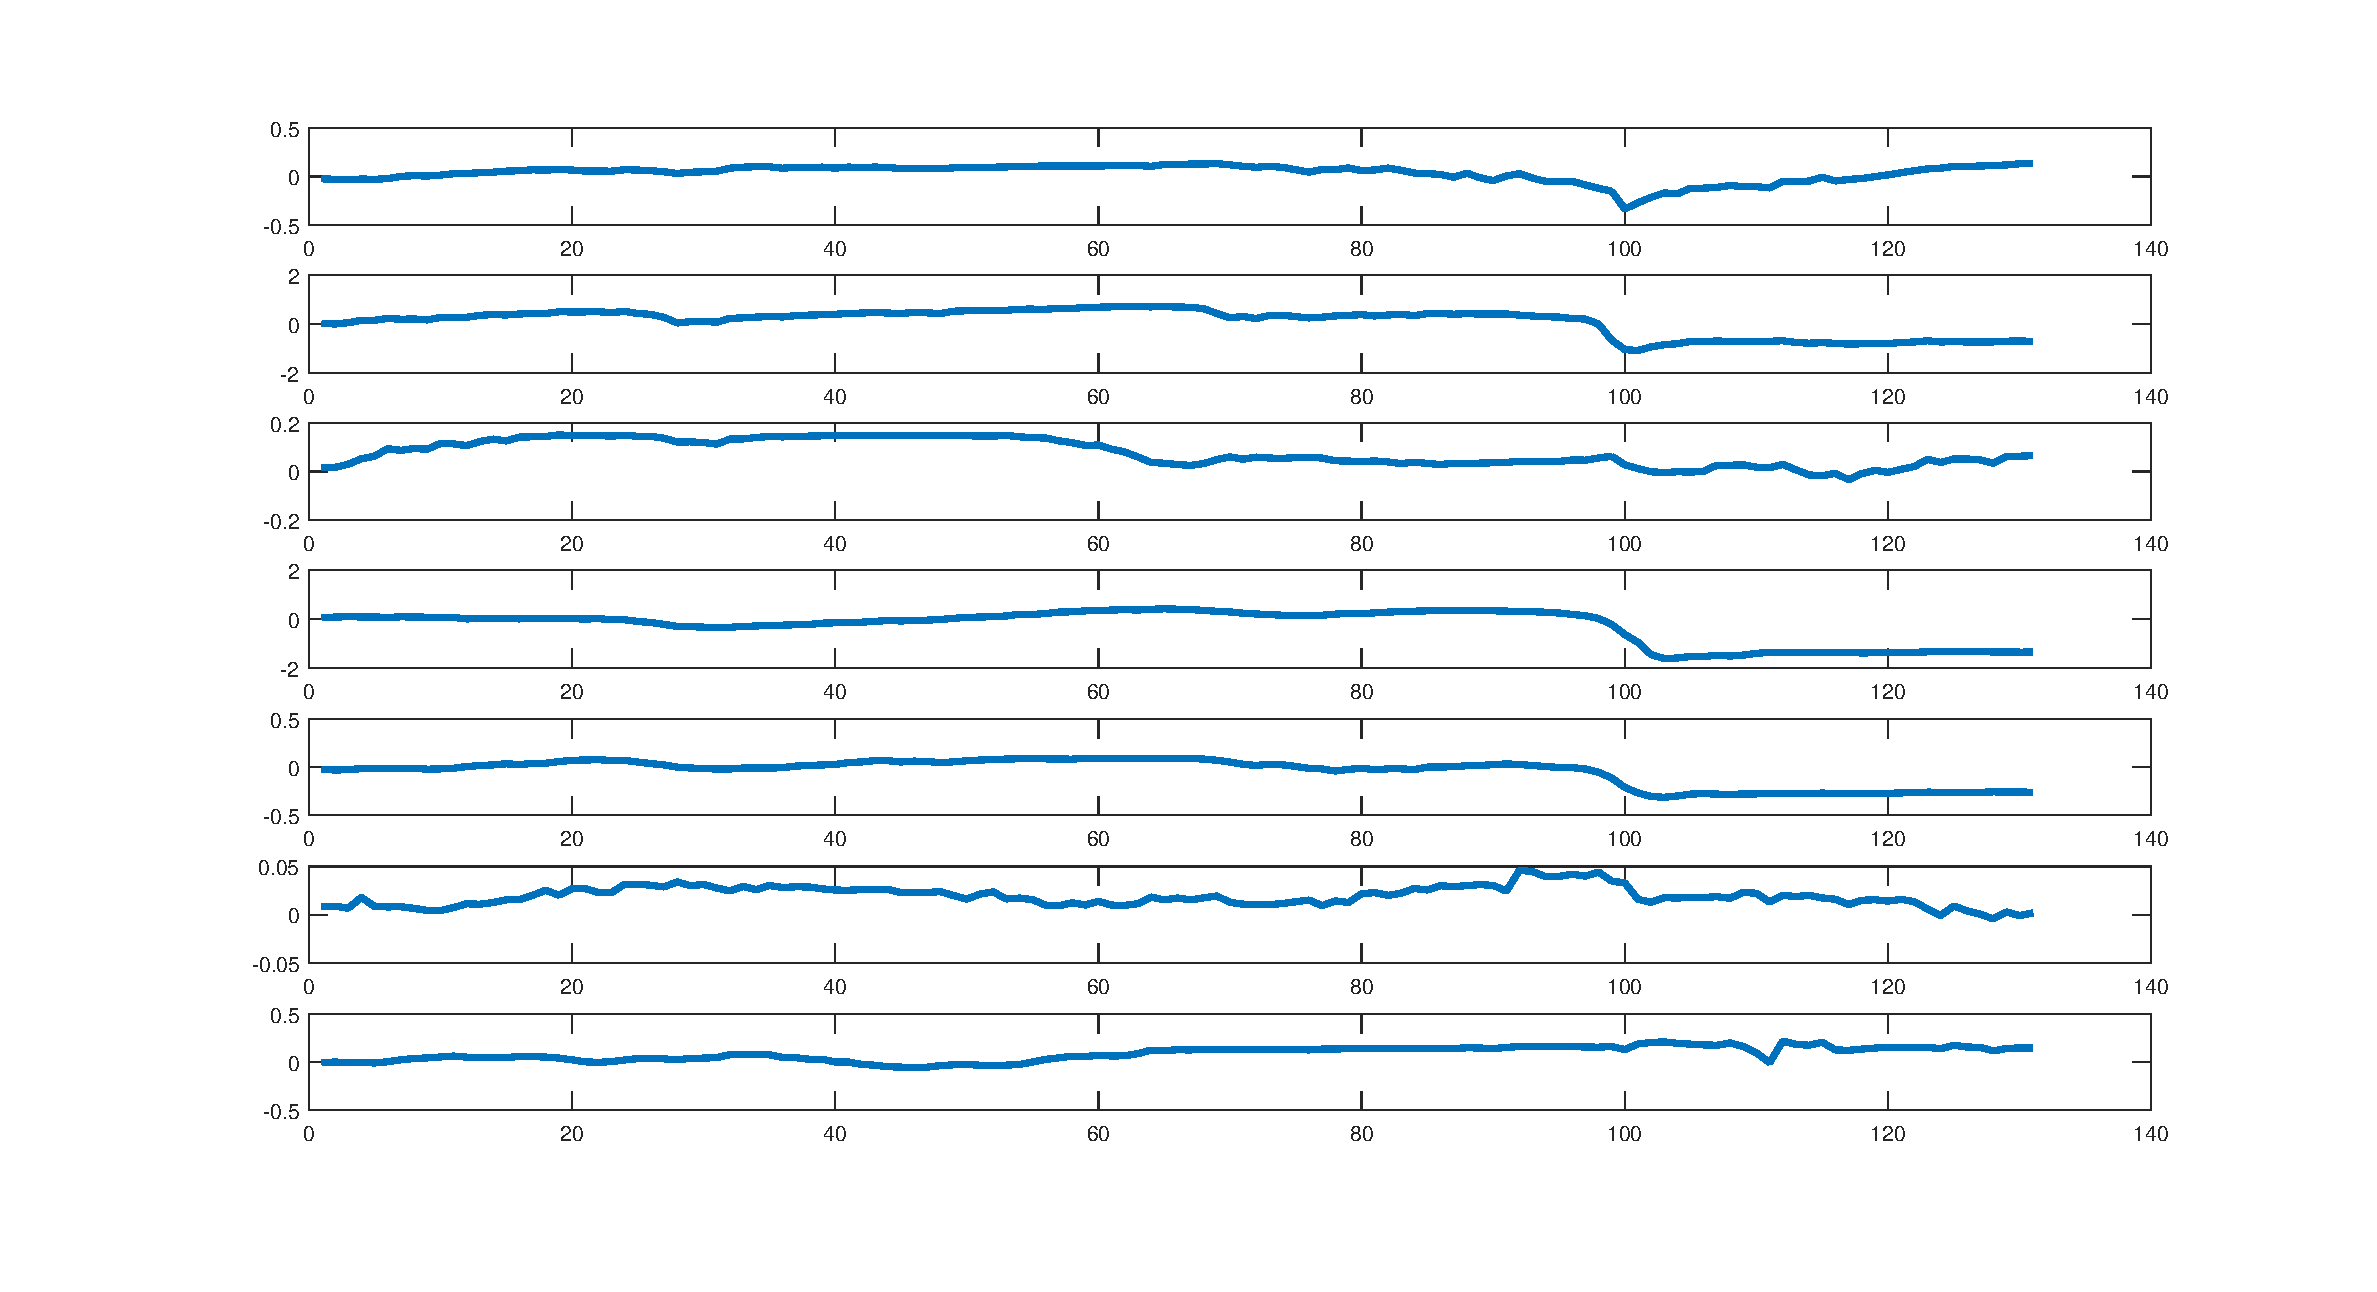
\includegraphics[scale=0.5]{sw_ar1_learning_alphas.pdf}\\
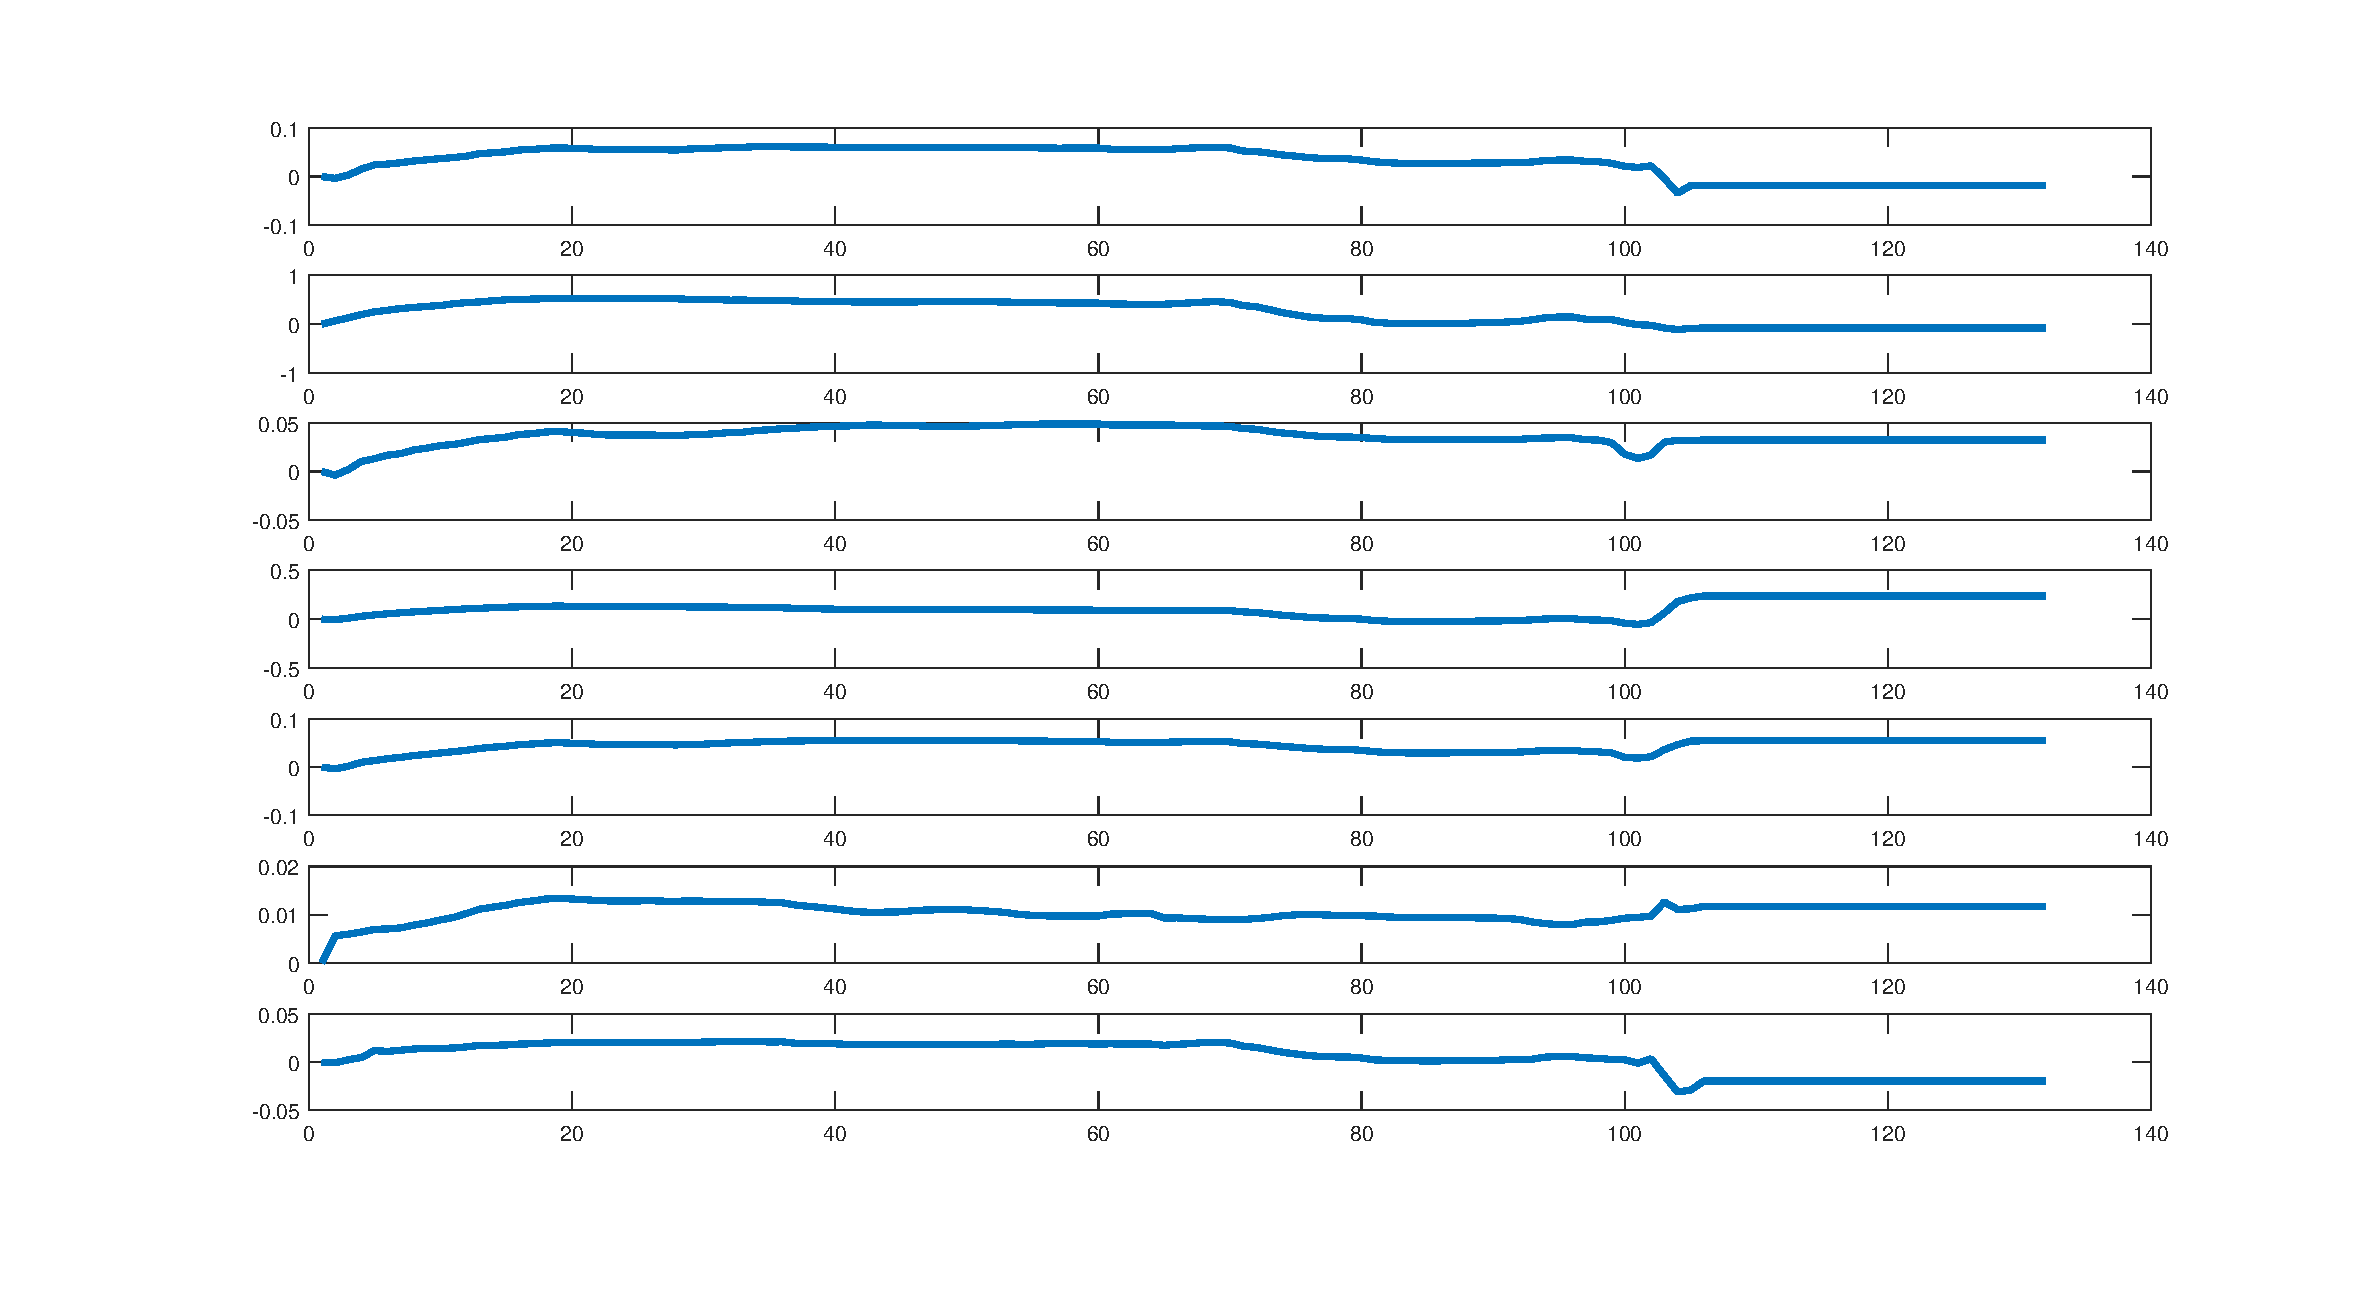
\includegraphics[scale=0.5]{sw_msv_learning_alphas.pdf}\\


\end{figure}



\begin{figure}[H]
\label{sw_learning_2}
\caption{Learning coefficients in the AR(1)- and MSV-learning cases: Persistence coefficients under AR(1)-learning, and lagged inflation under MSV-learning.} 
\vspace{5 mm}

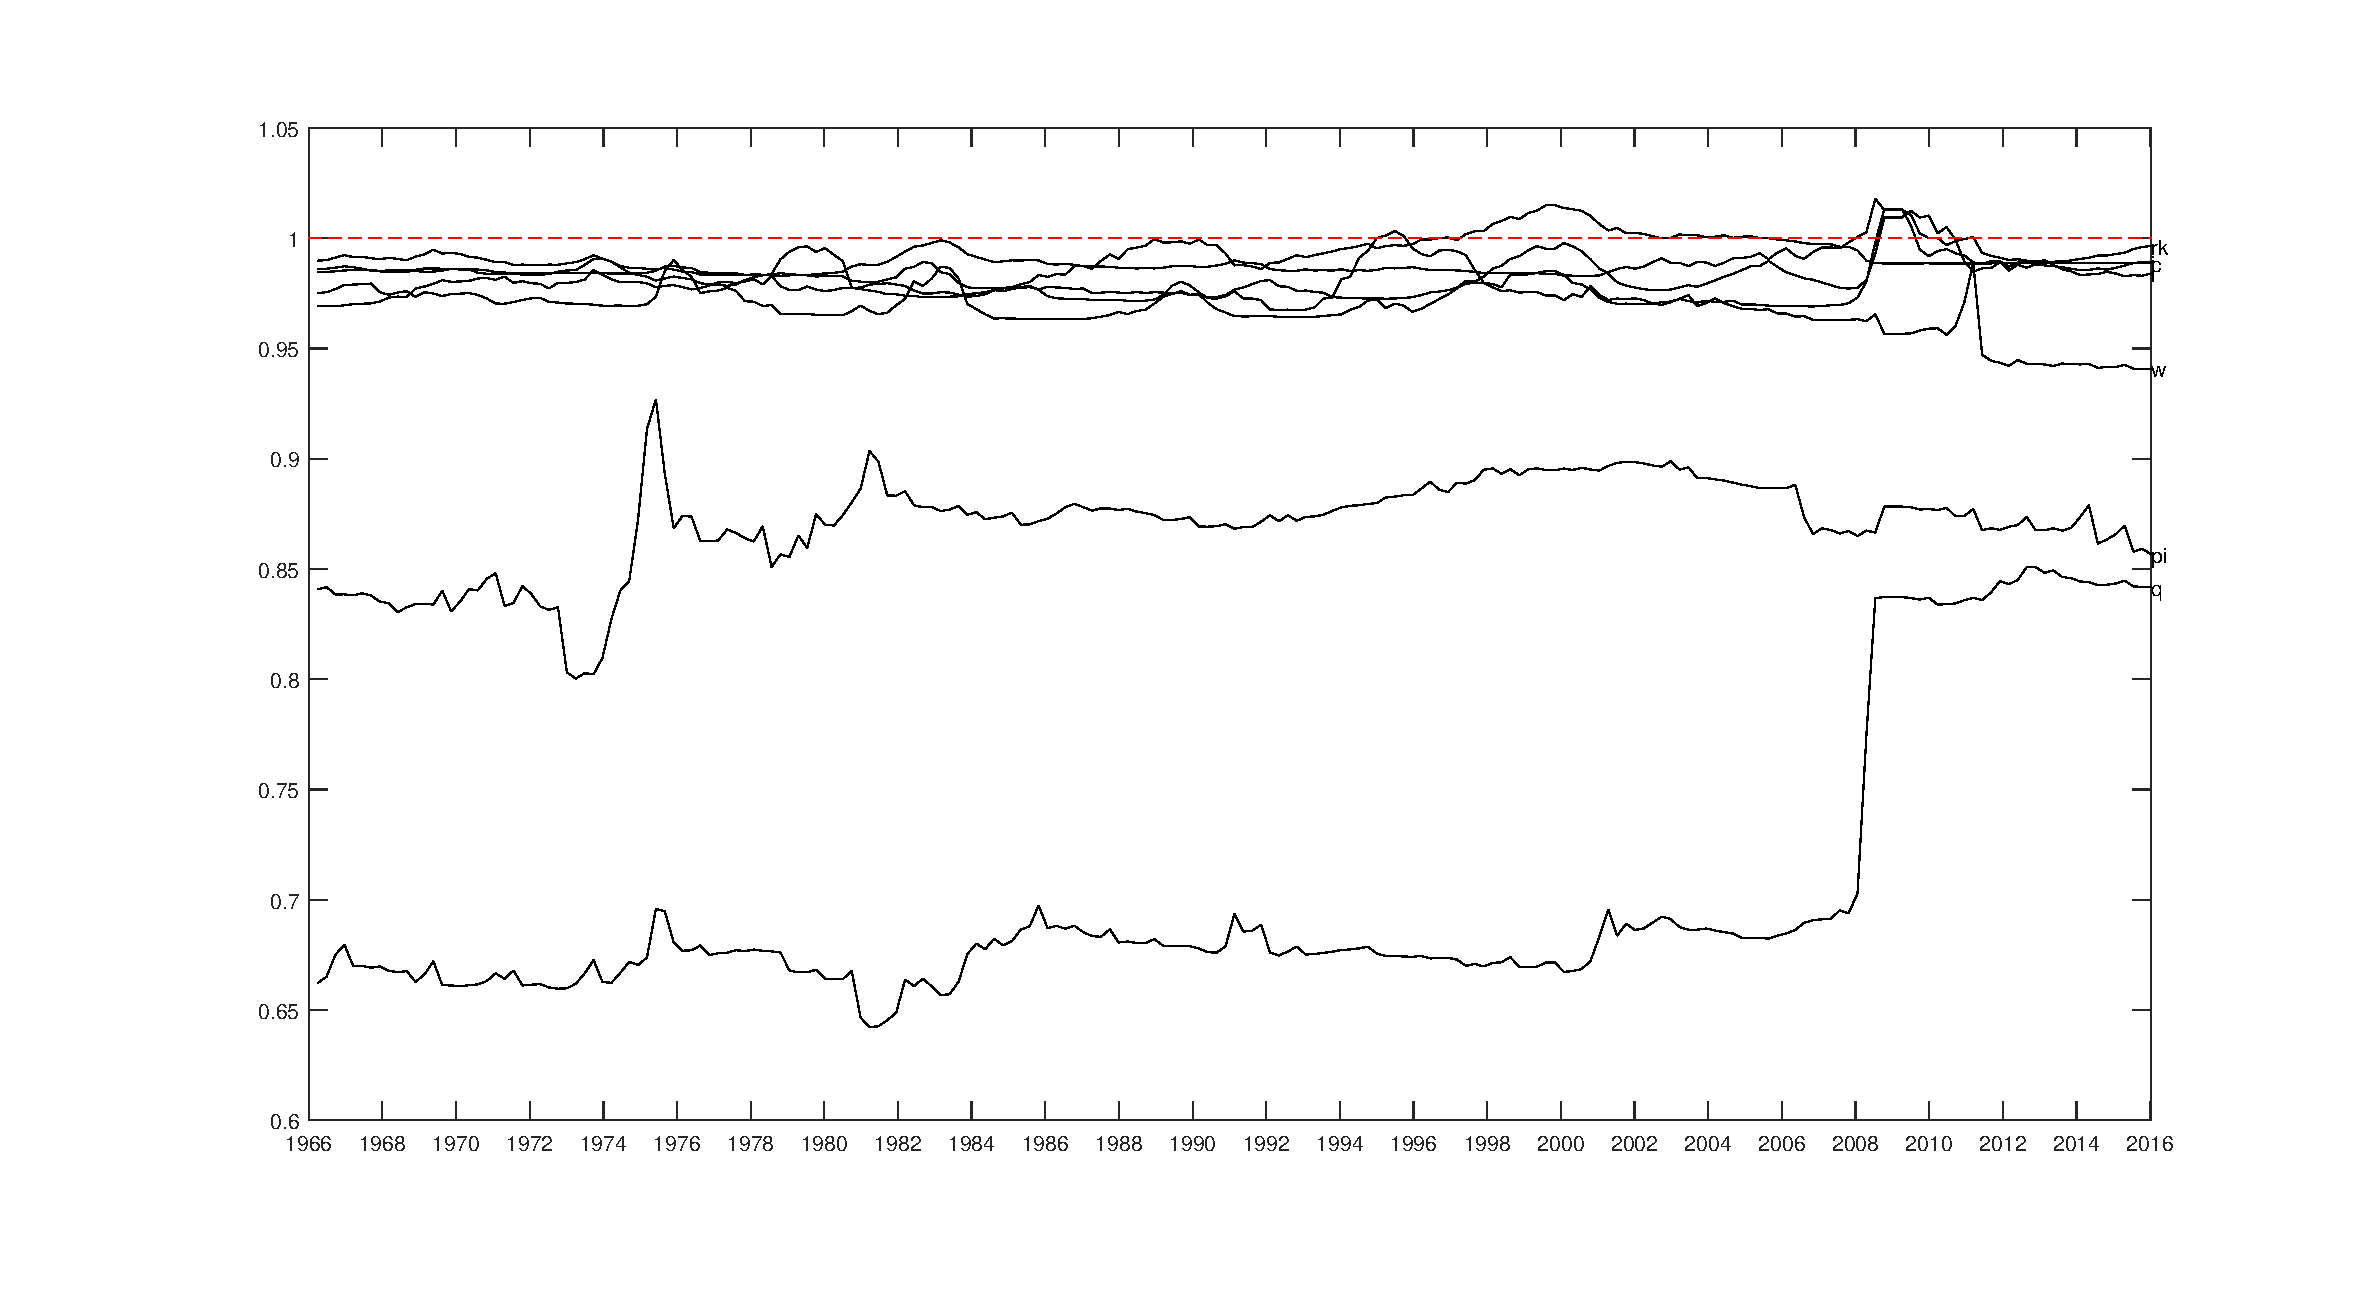
\includegraphics[scale=0.5]{sw_ar1_learning_betas.pdf}\\
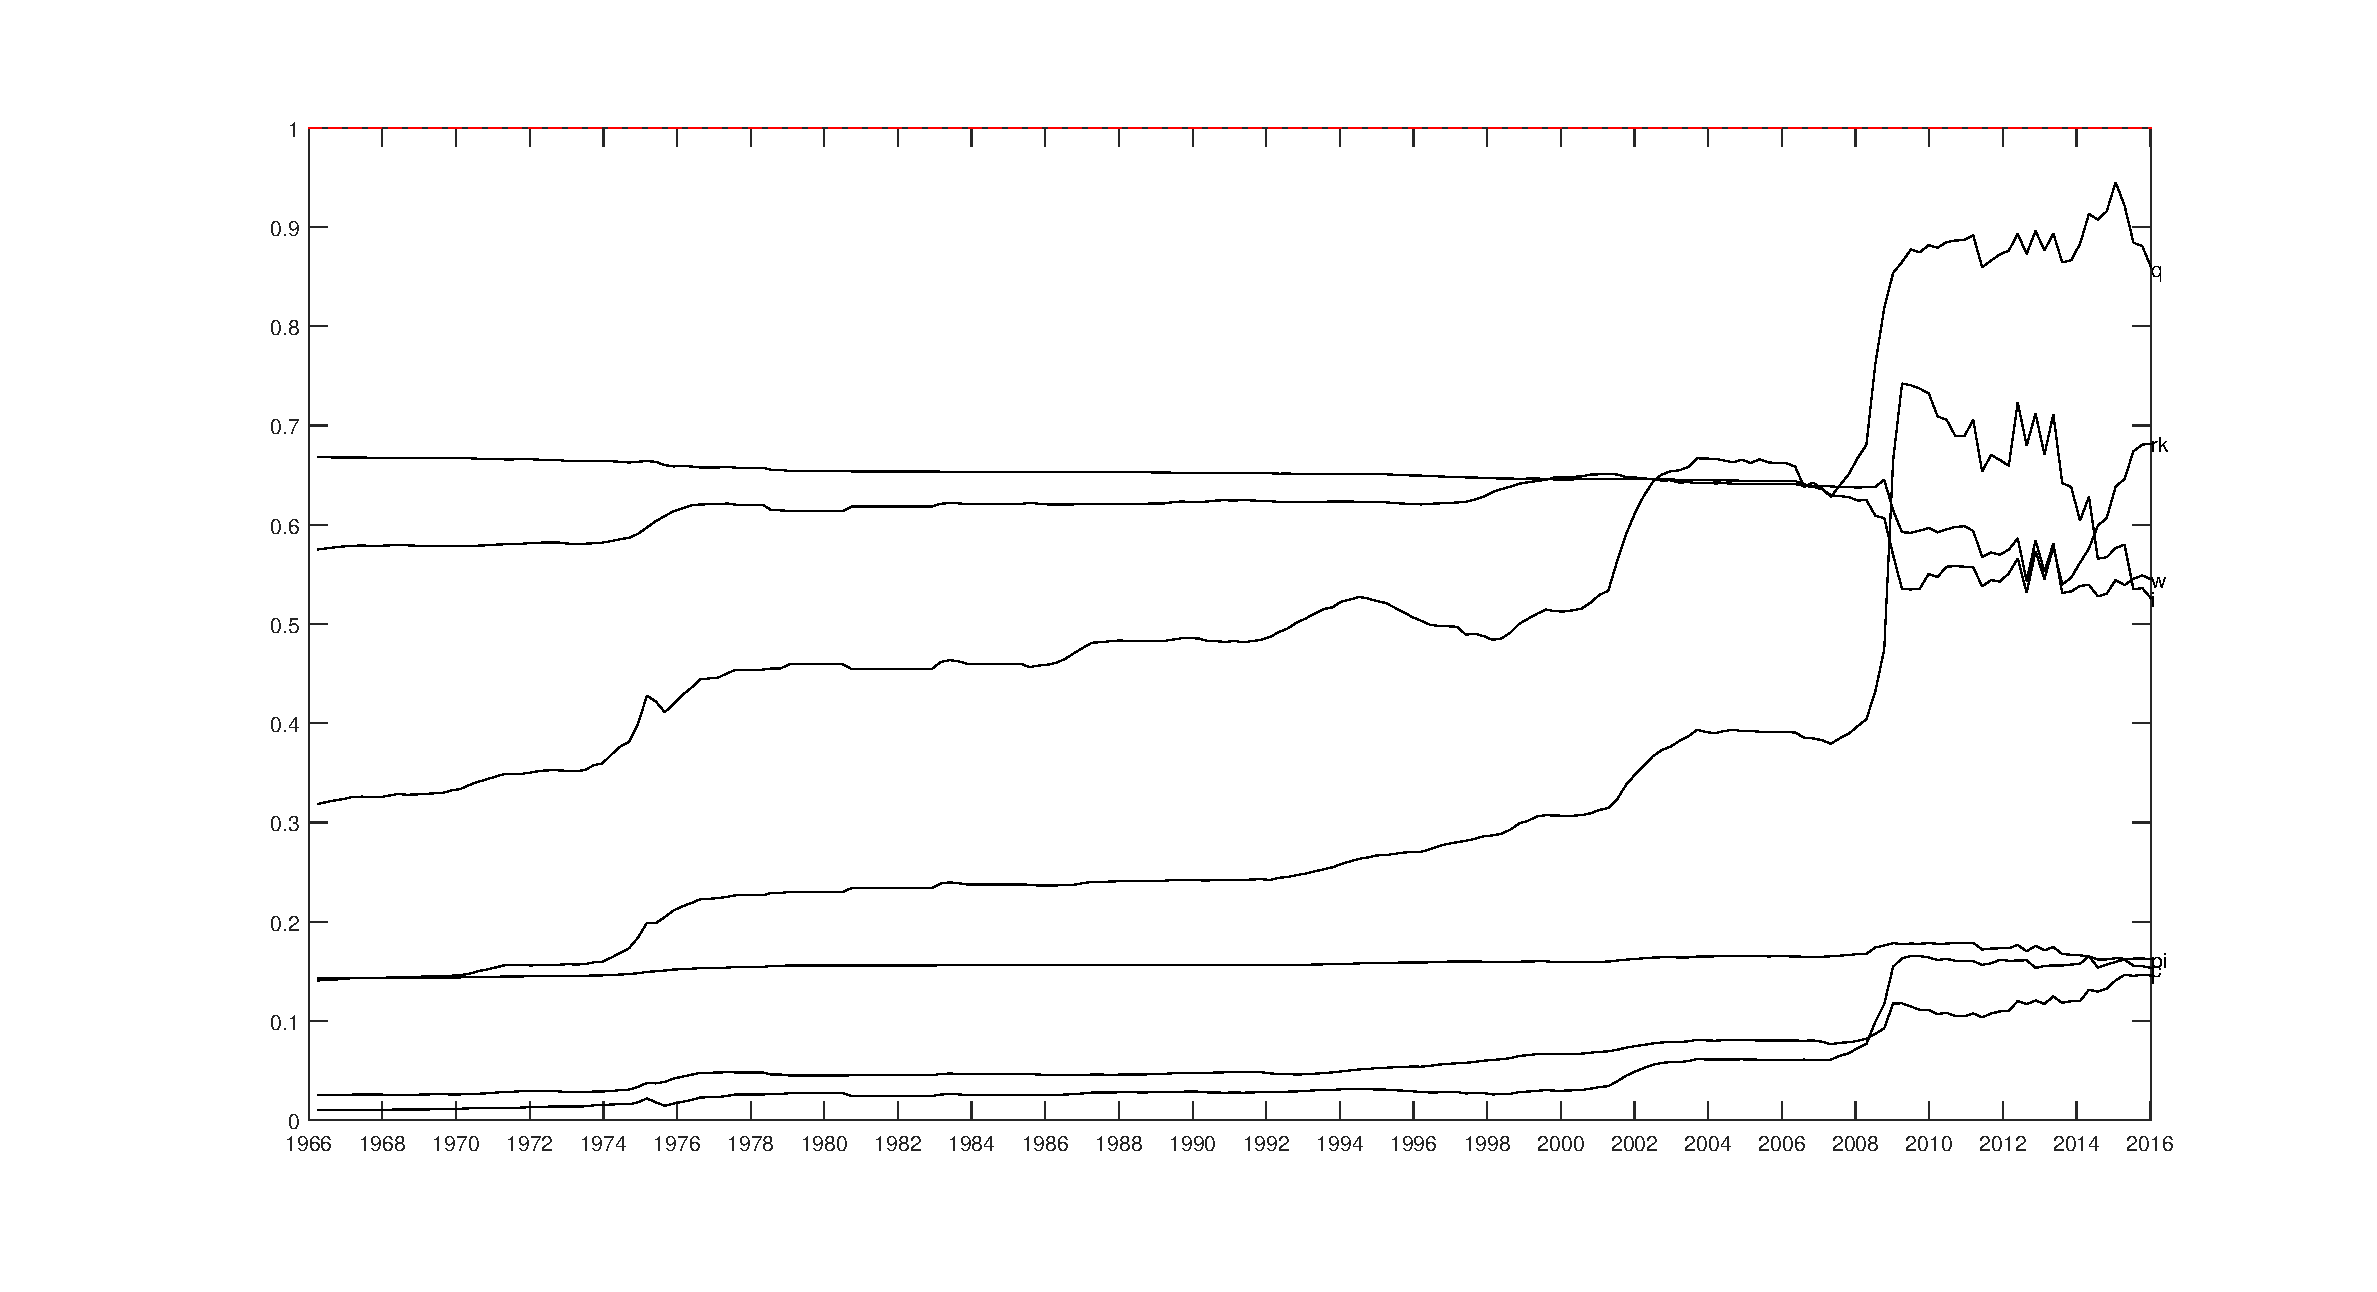
\includegraphics[scale=0.5]{sw_msv_learning_laggedInfl.pdf}\\
\end{figure}


\subsection{Forecast Errors}

\begin{figure}[H]

\caption{In-sample forecasts (i.e. the forecasting step of the filter) for all observables.}
\vspace{5 mm}

\textbf{MS-REE and REE: }\\
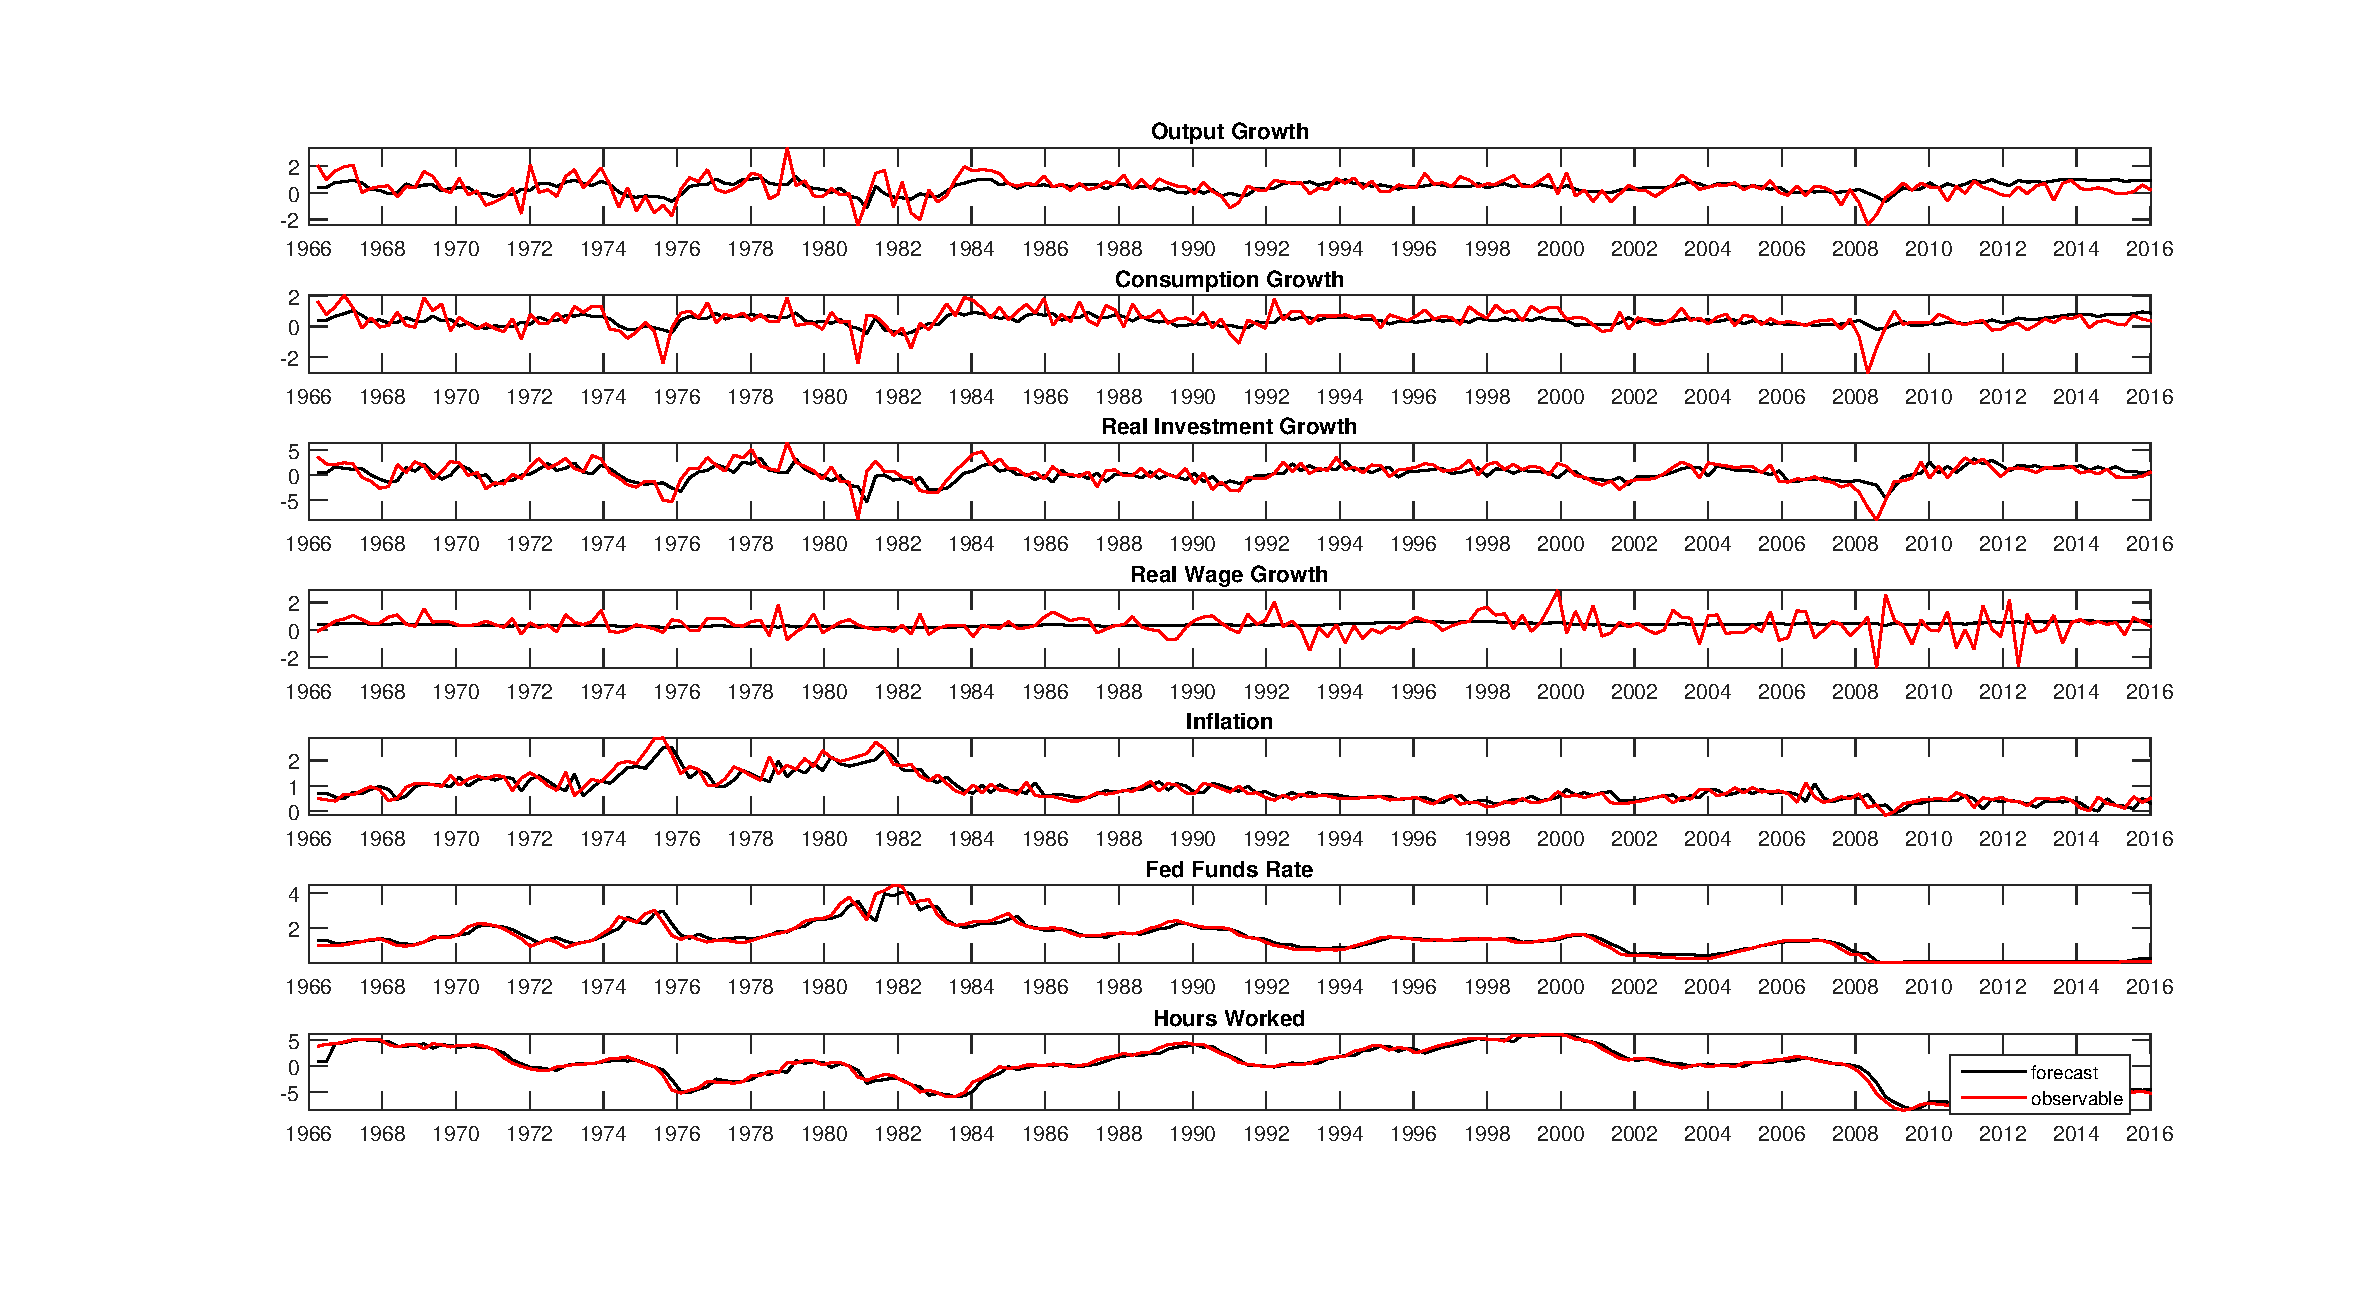
\includegraphics[height=.5\textheight,width=.5\textwidth]{rise_forecast_errors.pdf}
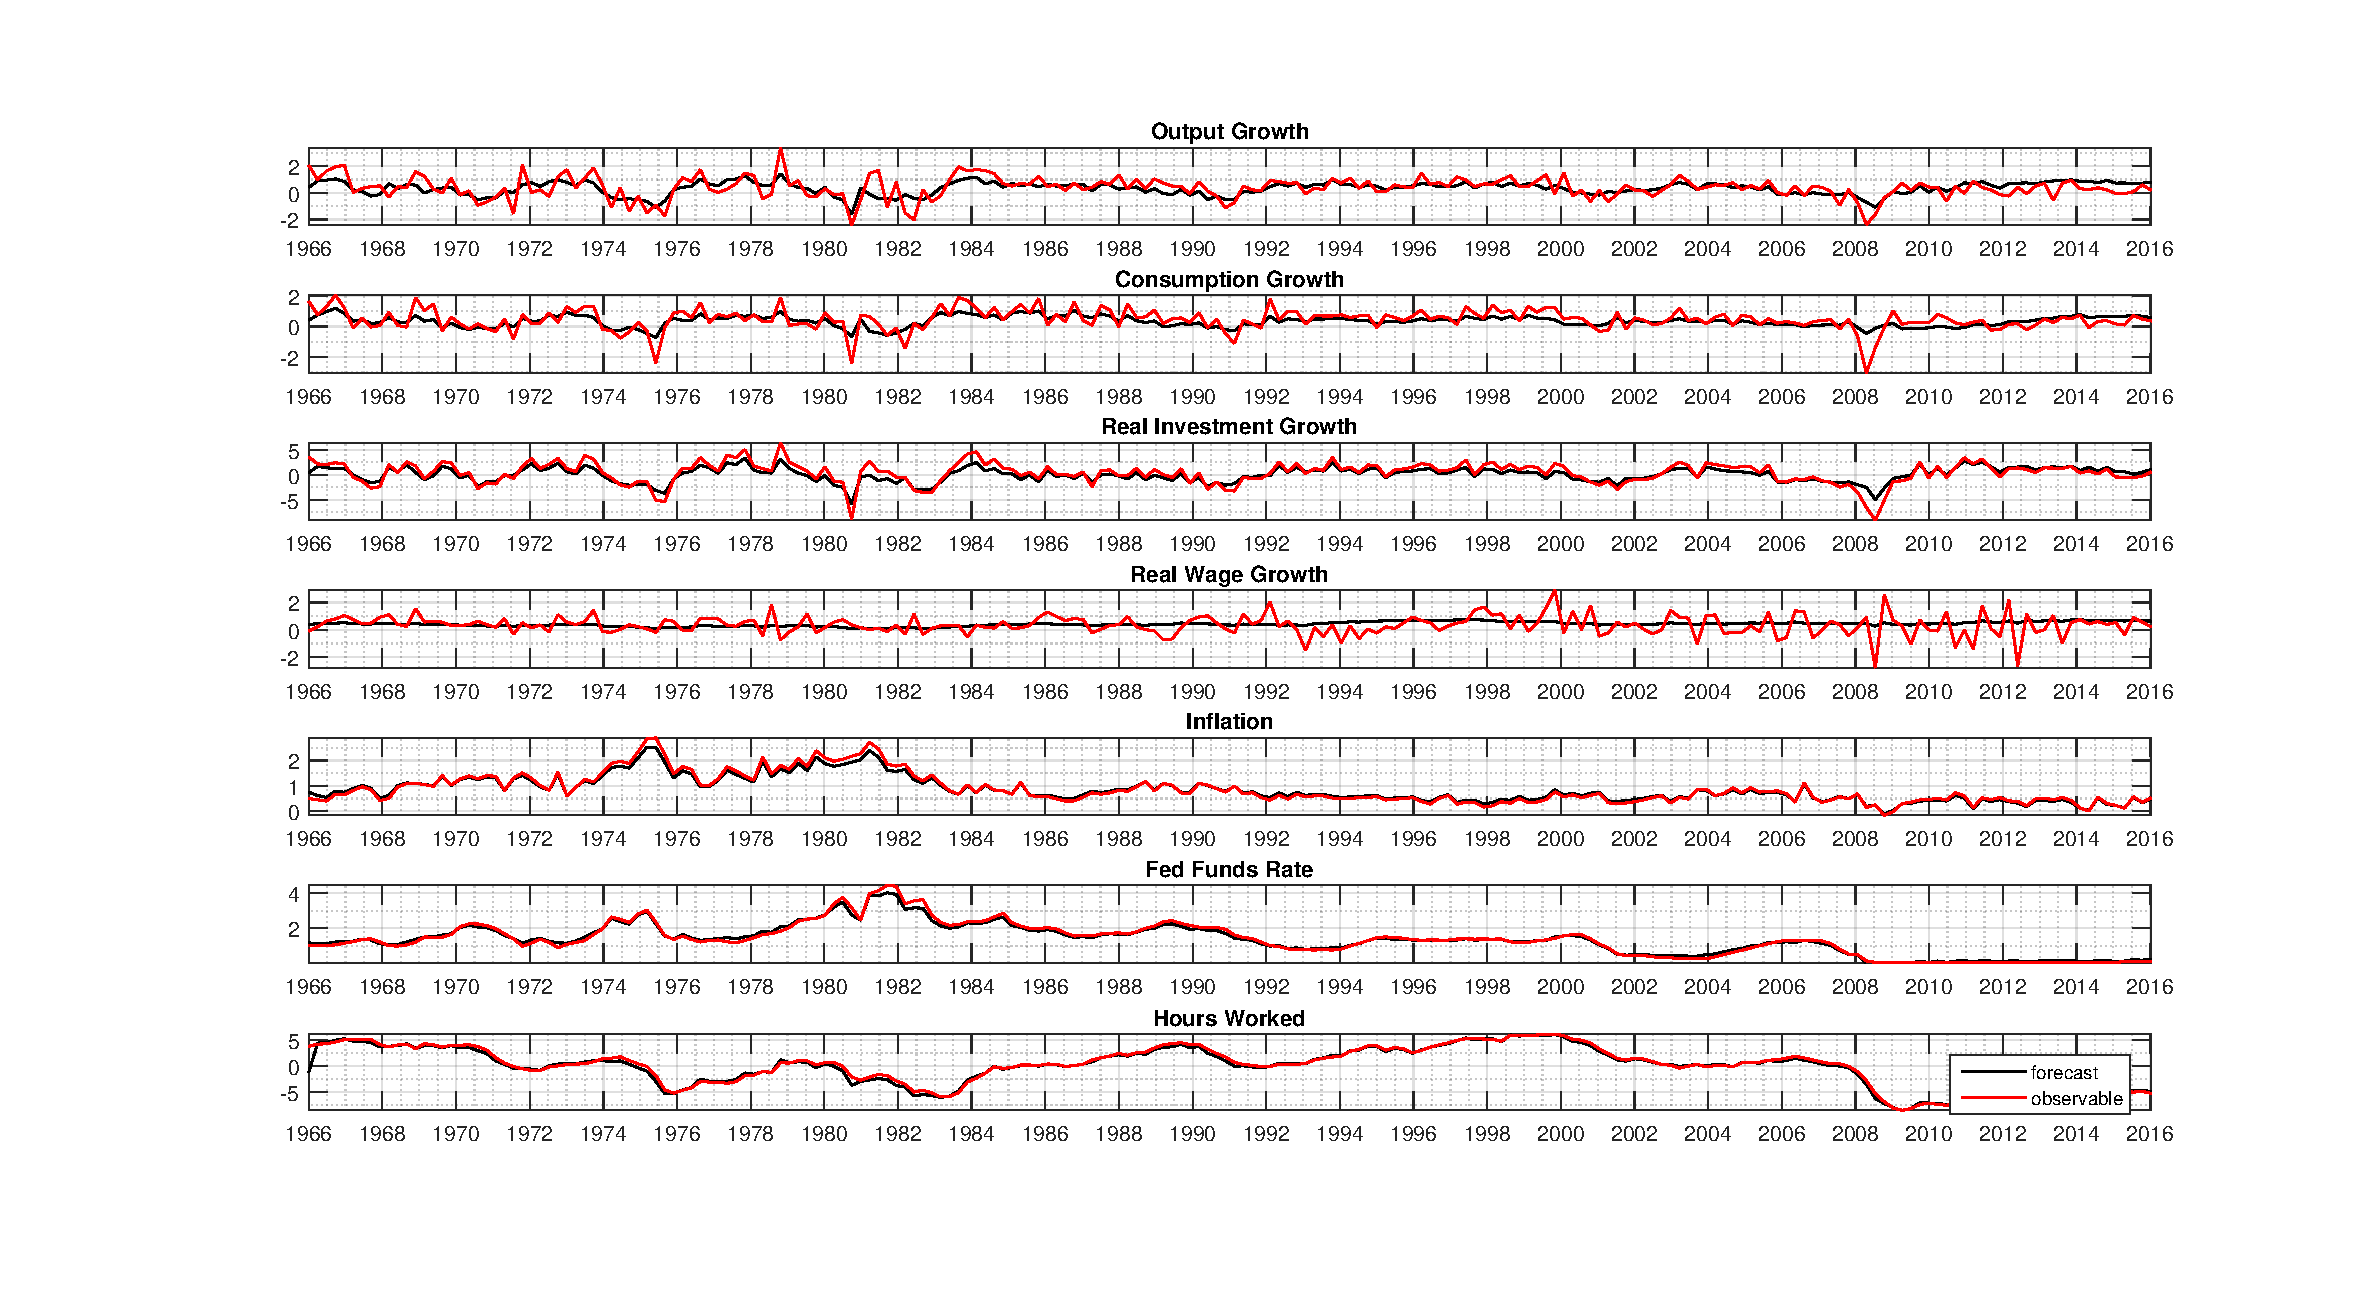
\includegraphics[height=.5\textheight,width=.5\textwidth]{REE_forecast_errors.pdf}


\textbf{MSV- and AR(1)-learning: }\\
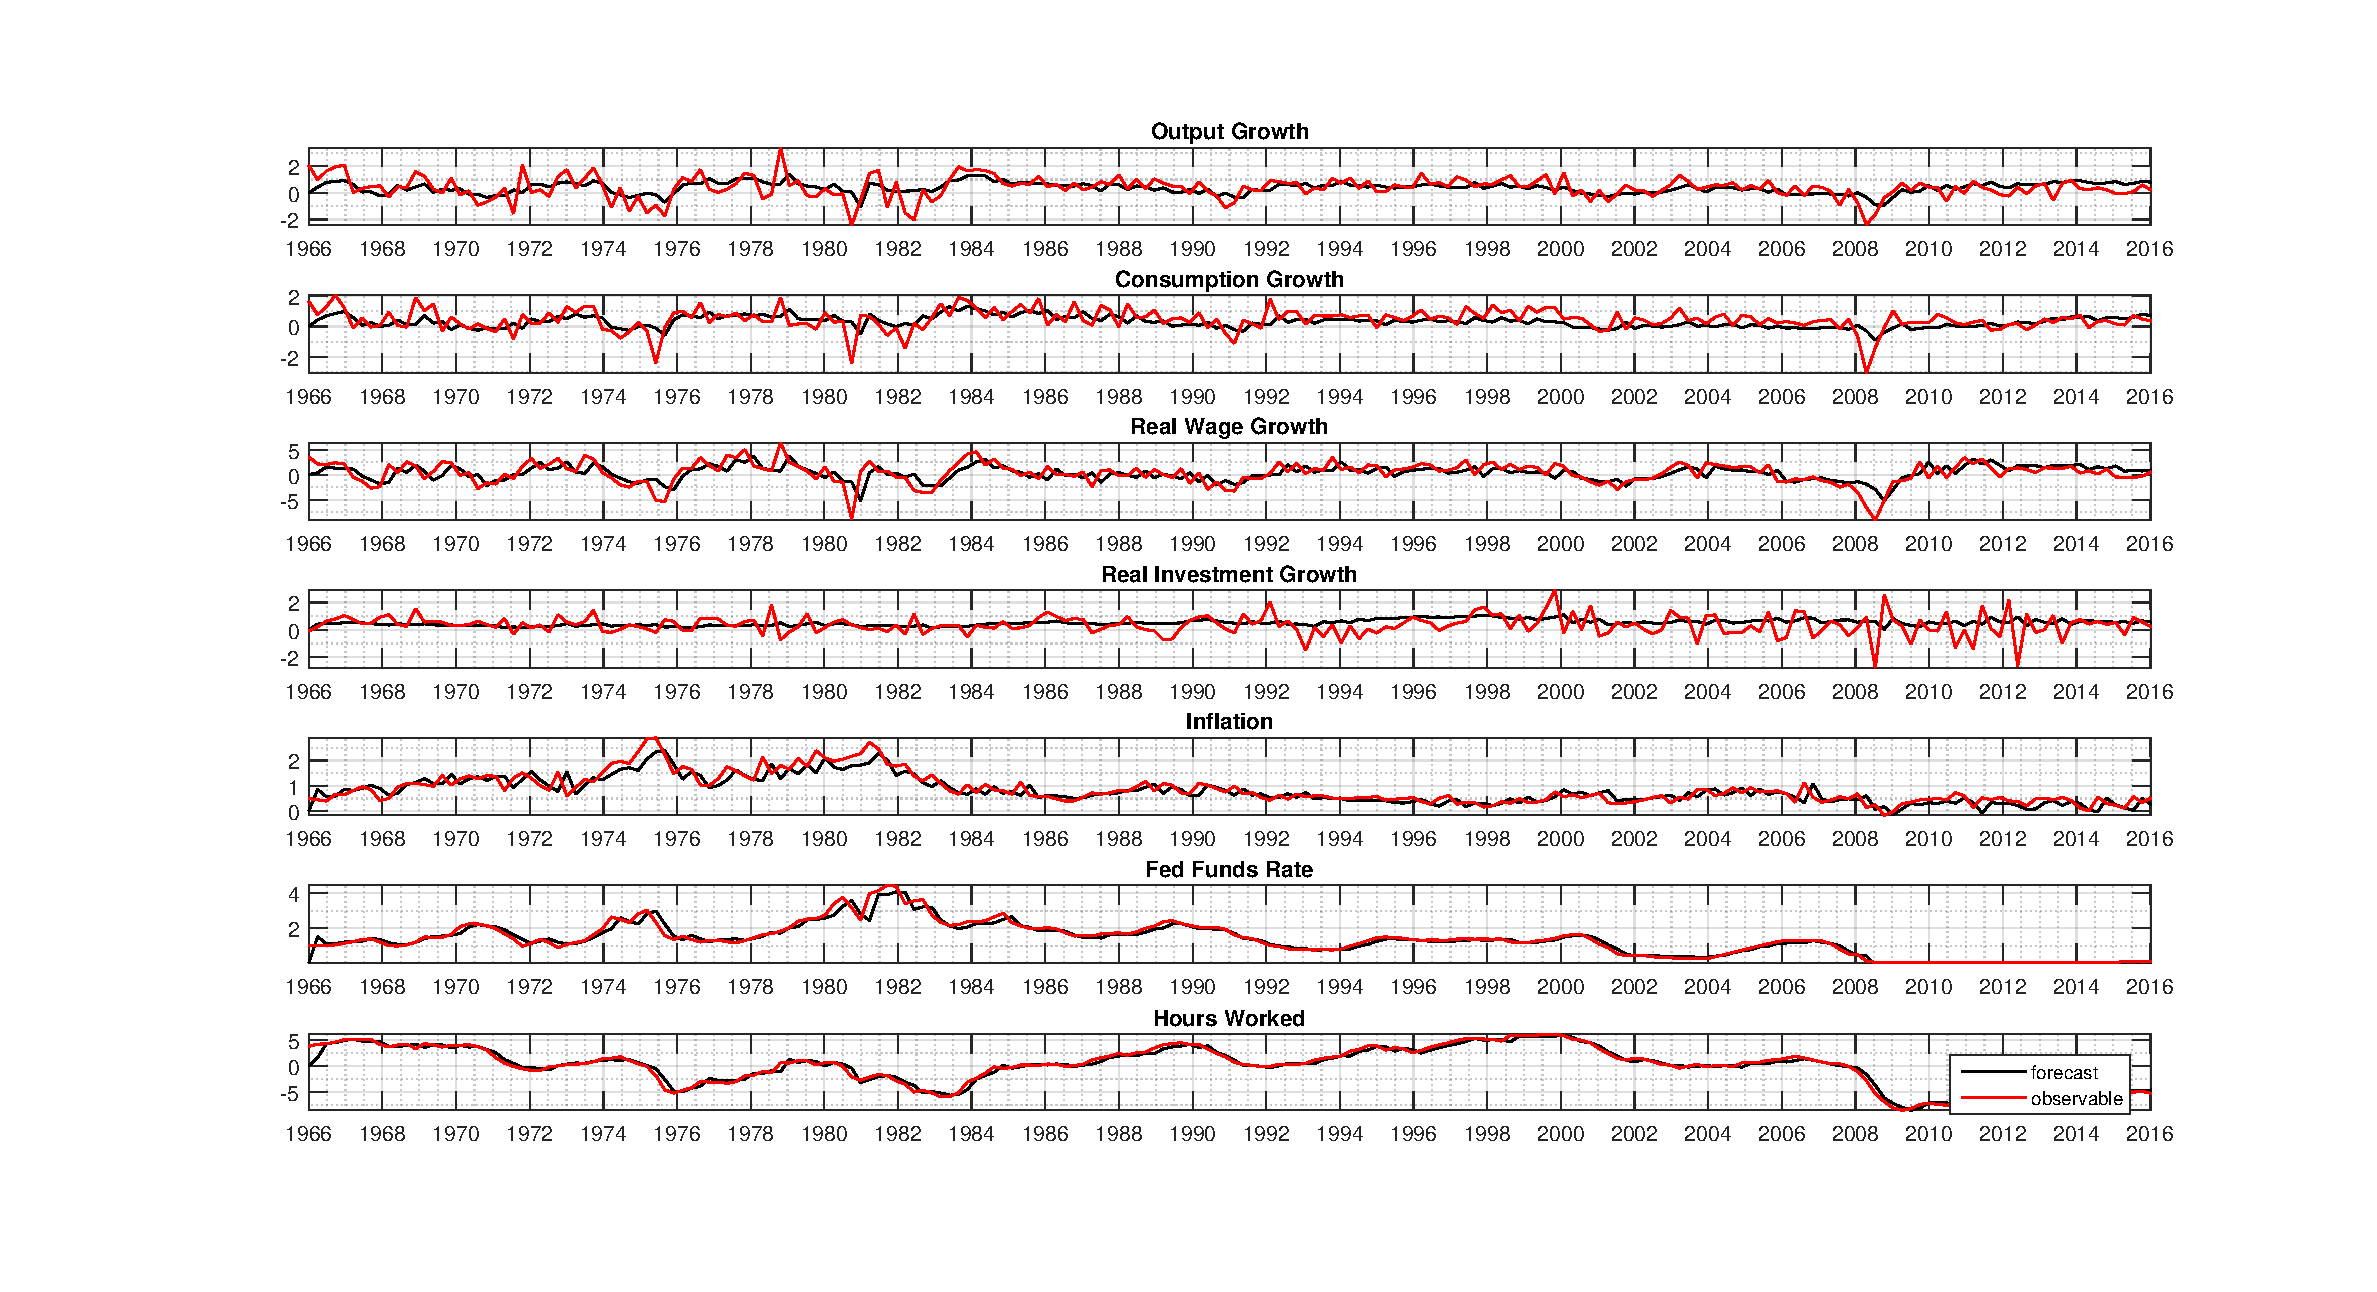
\includegraphics[height=.5\textheight,width=.5\textwidth]{sw_msv_forecast_errors.pdf}
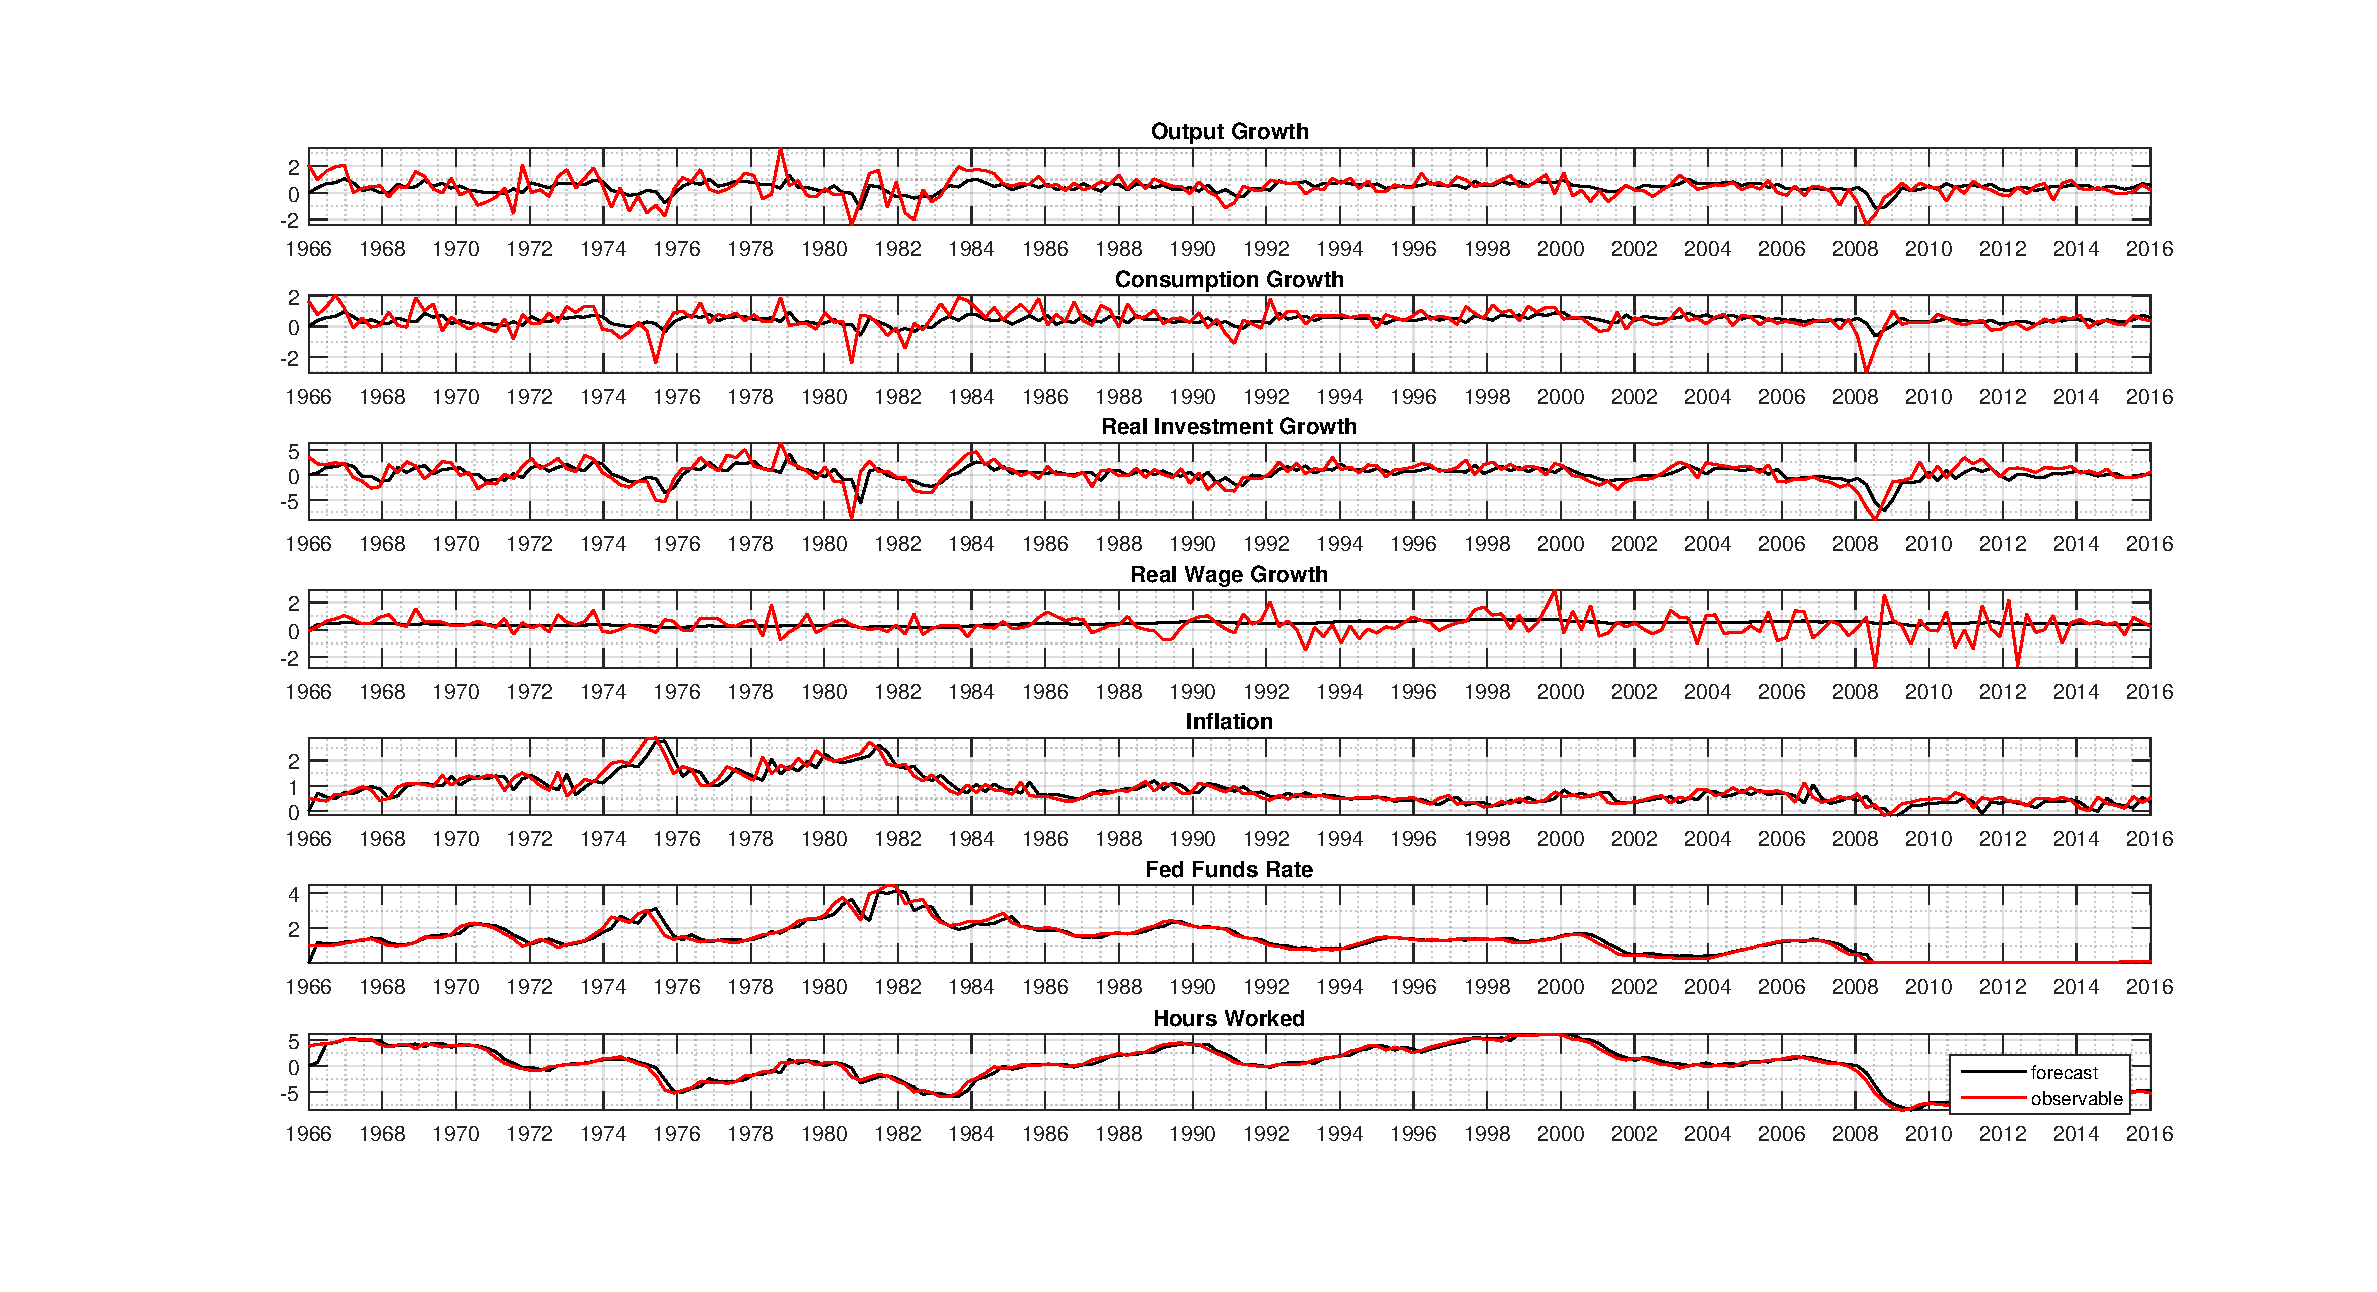
\includegraphics[height=0.5\textheight,width=0.5\textwidth]{sw_ar1_forecast_errors.pdf}



\end{figure}


\subsection{Impulse Responses: Comparison with MS-REE and implied time-variation}



\begin{figure}[H]
\caption{Comparison of AR(1) learning IRFs with RISE IRFs. One unit shocks of $\eta_a$,$\eta_b$,$\eta_g$,$\eta_i$,$\eta_p$,$\eta_w$ respectively.}
\textbf{Consumption:}\\
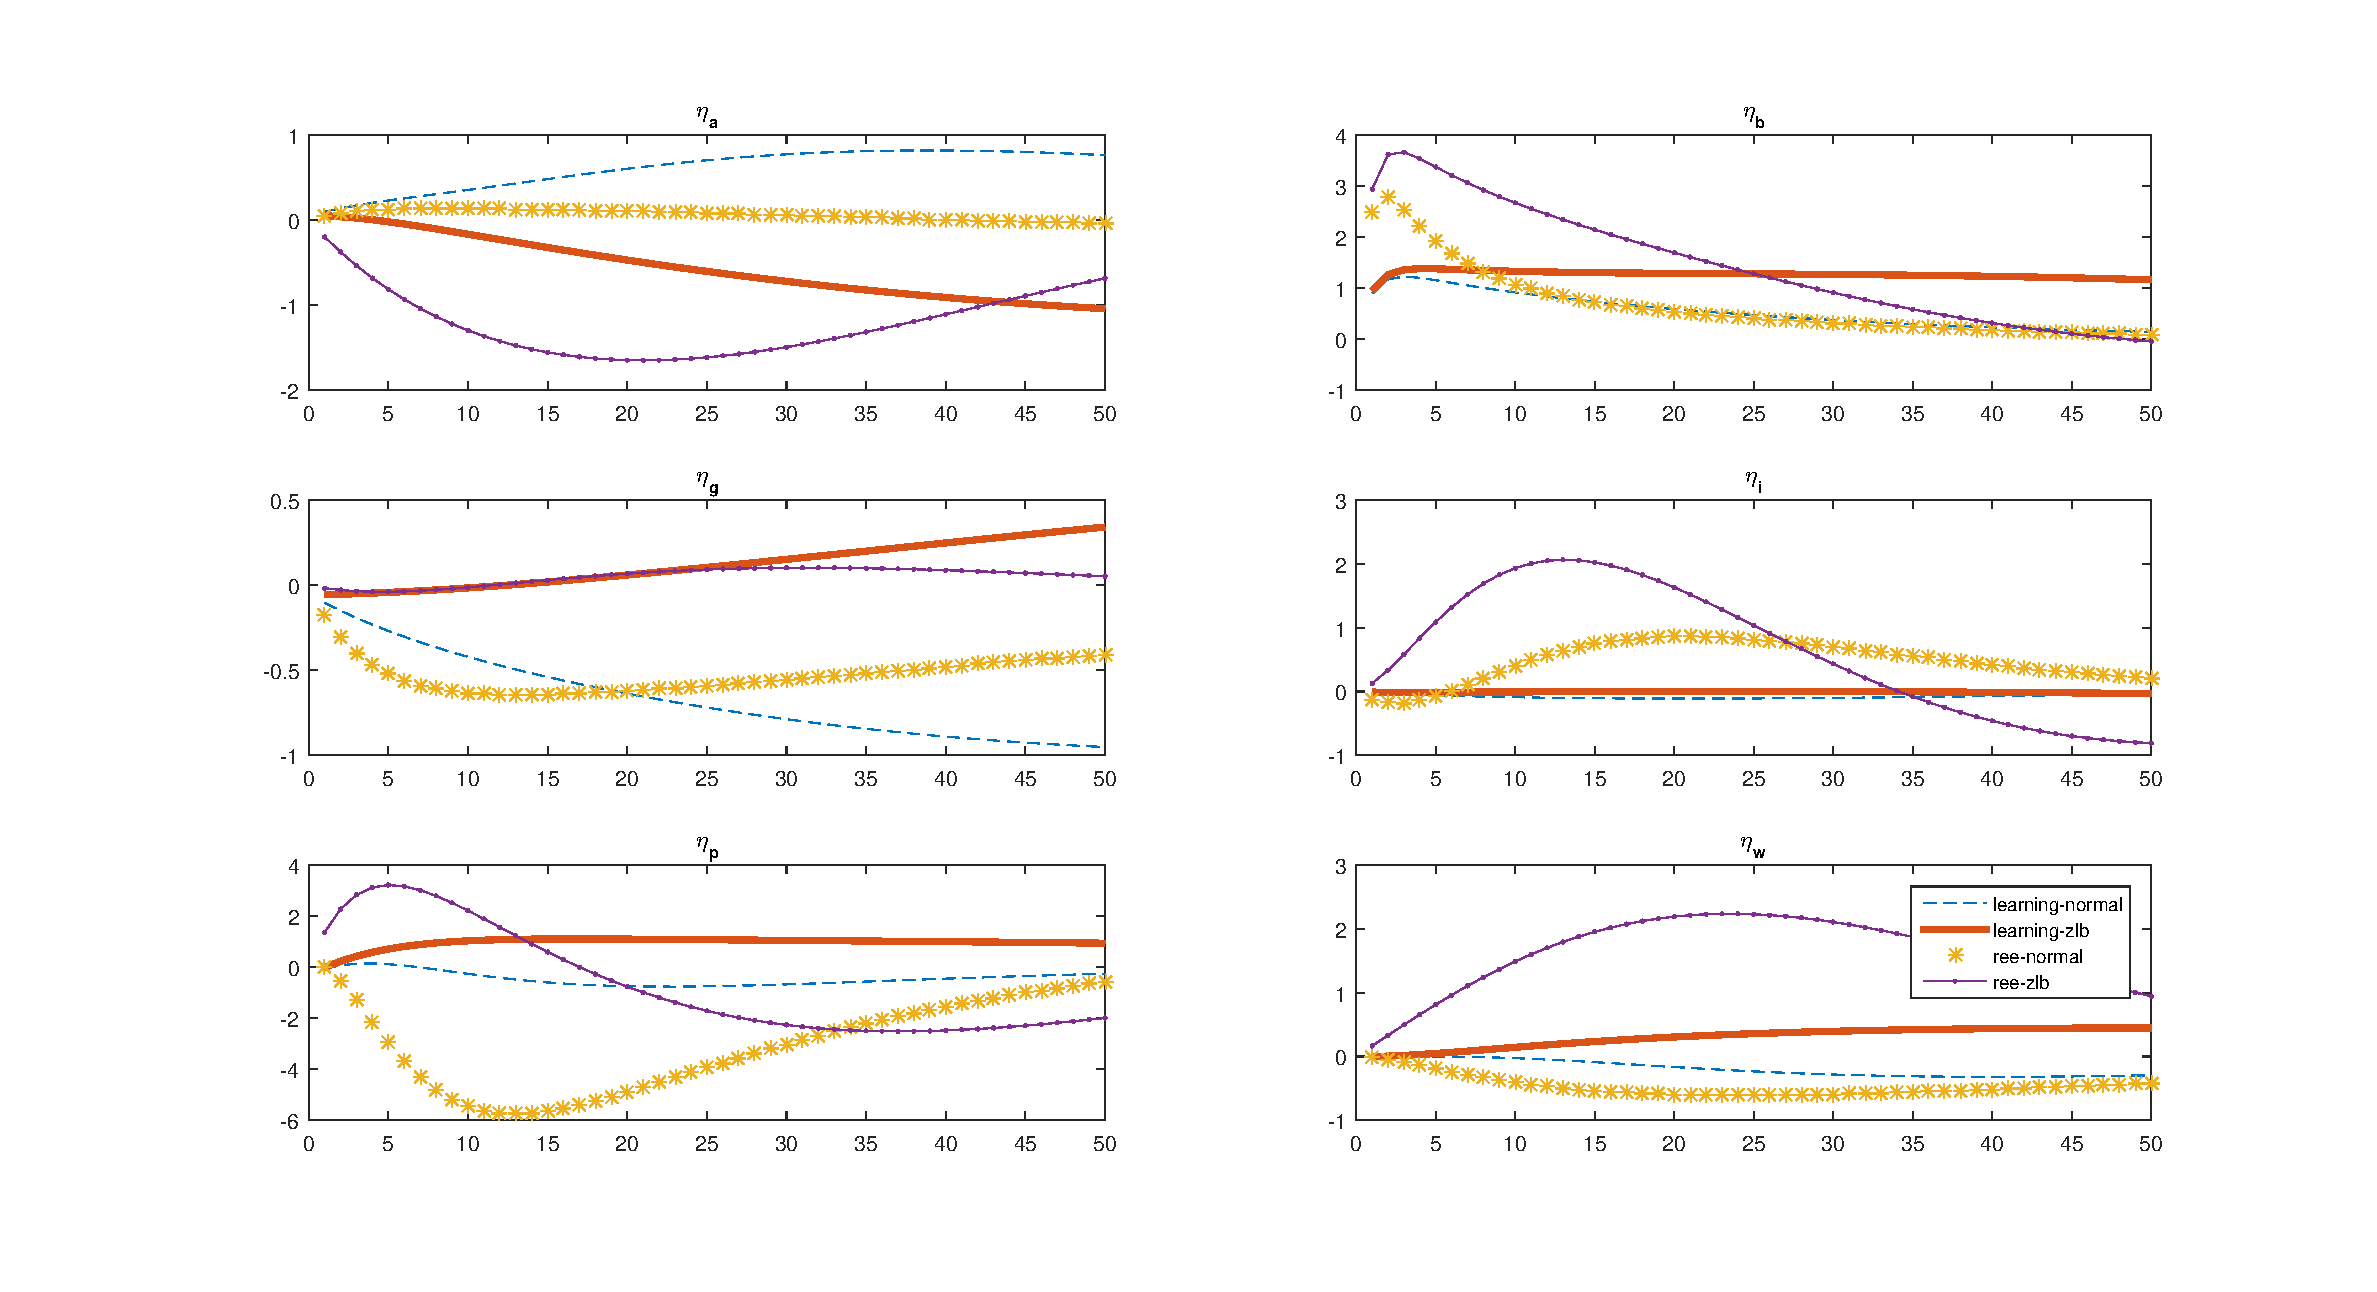
\includegraphics[scale=0.5]{AR1_impresp_cons_riseComp.pdf}
\textbf{Investment:}\\
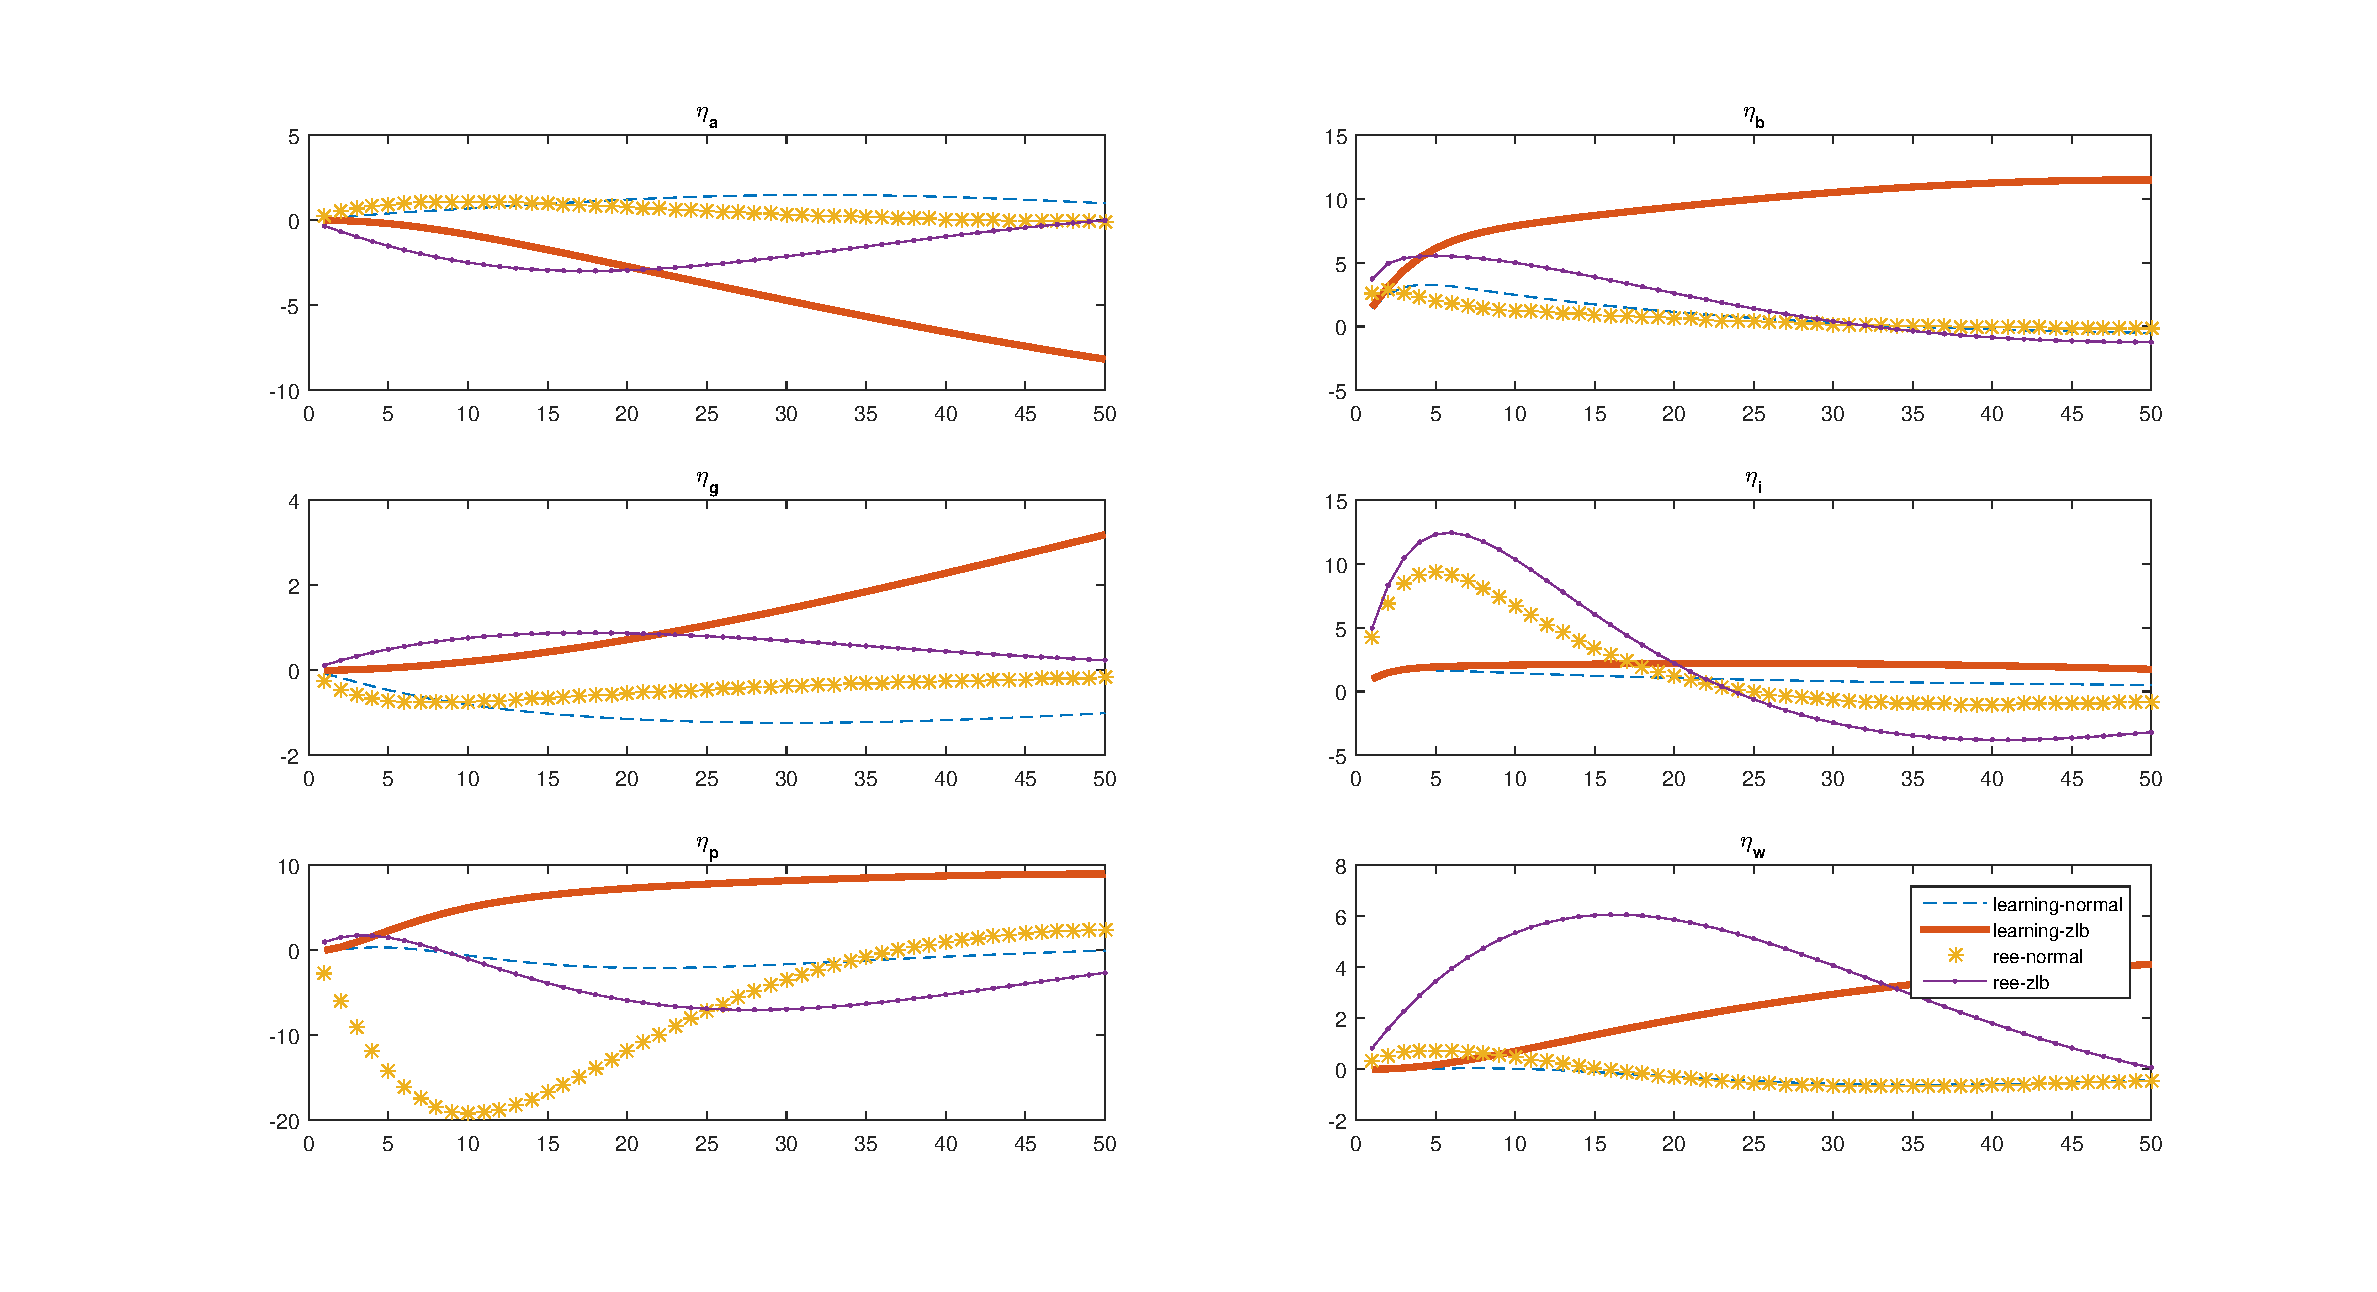
\includegraphics[scale=0.5]{AR1_impresp_inv_riseComp.pdf}

\end{figure}

\begin{figure}[H]
\textbf{Output:}\\
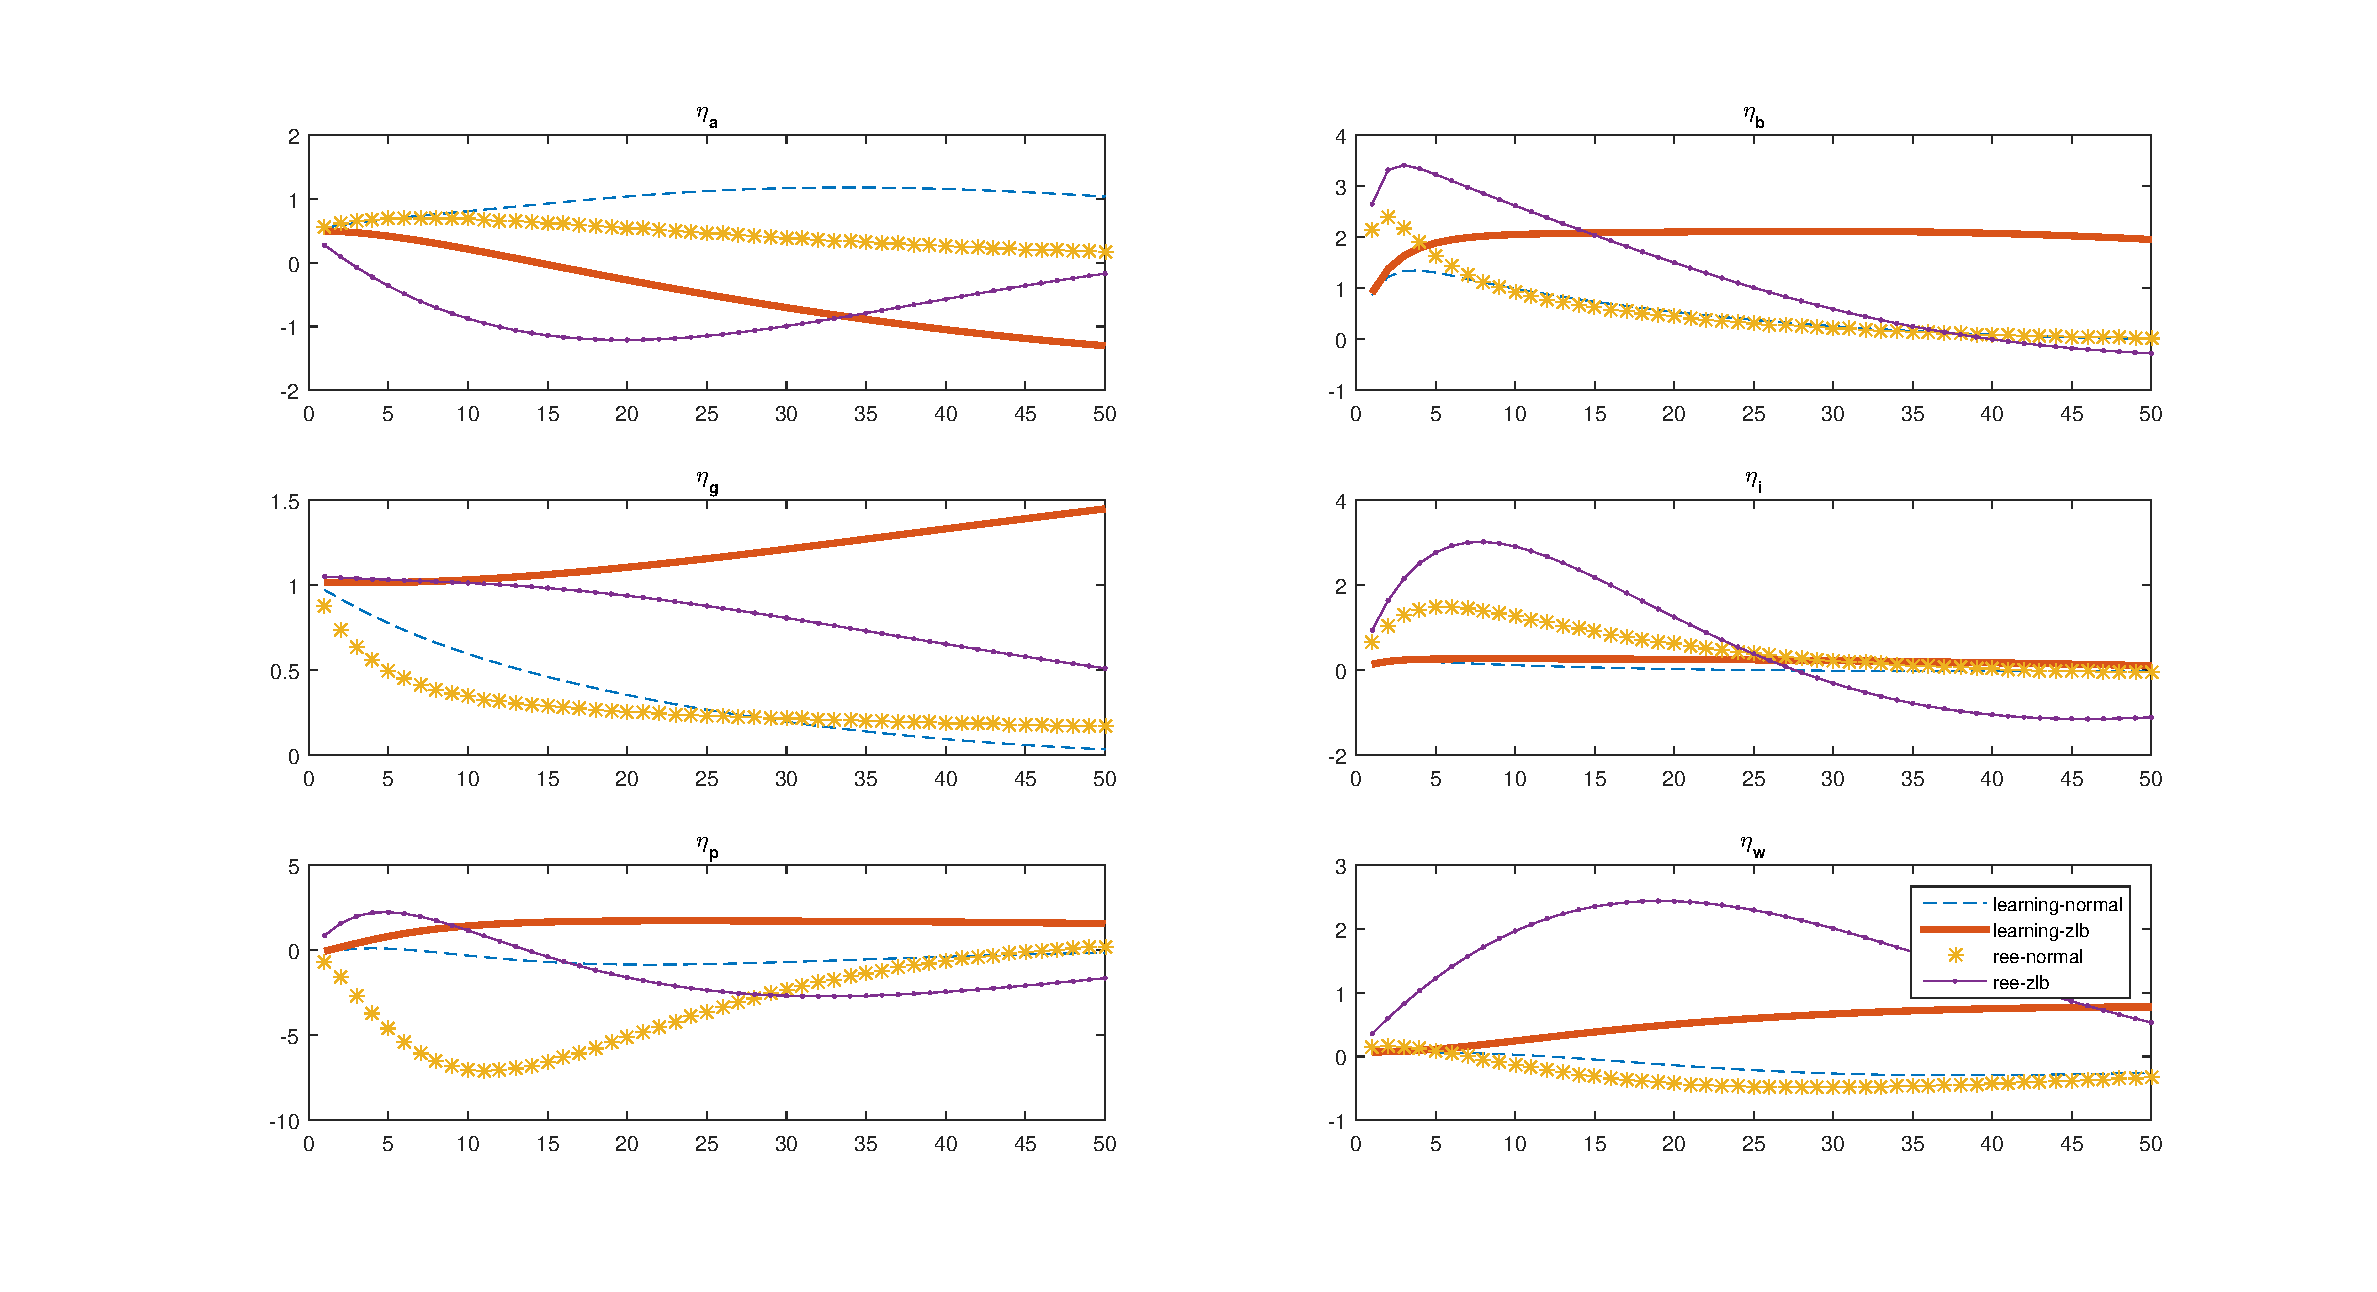
\includegraphics[scale=0.5]{AR1_impresp_output_riseComp.pdf}
\textbf{Inflation:}\\
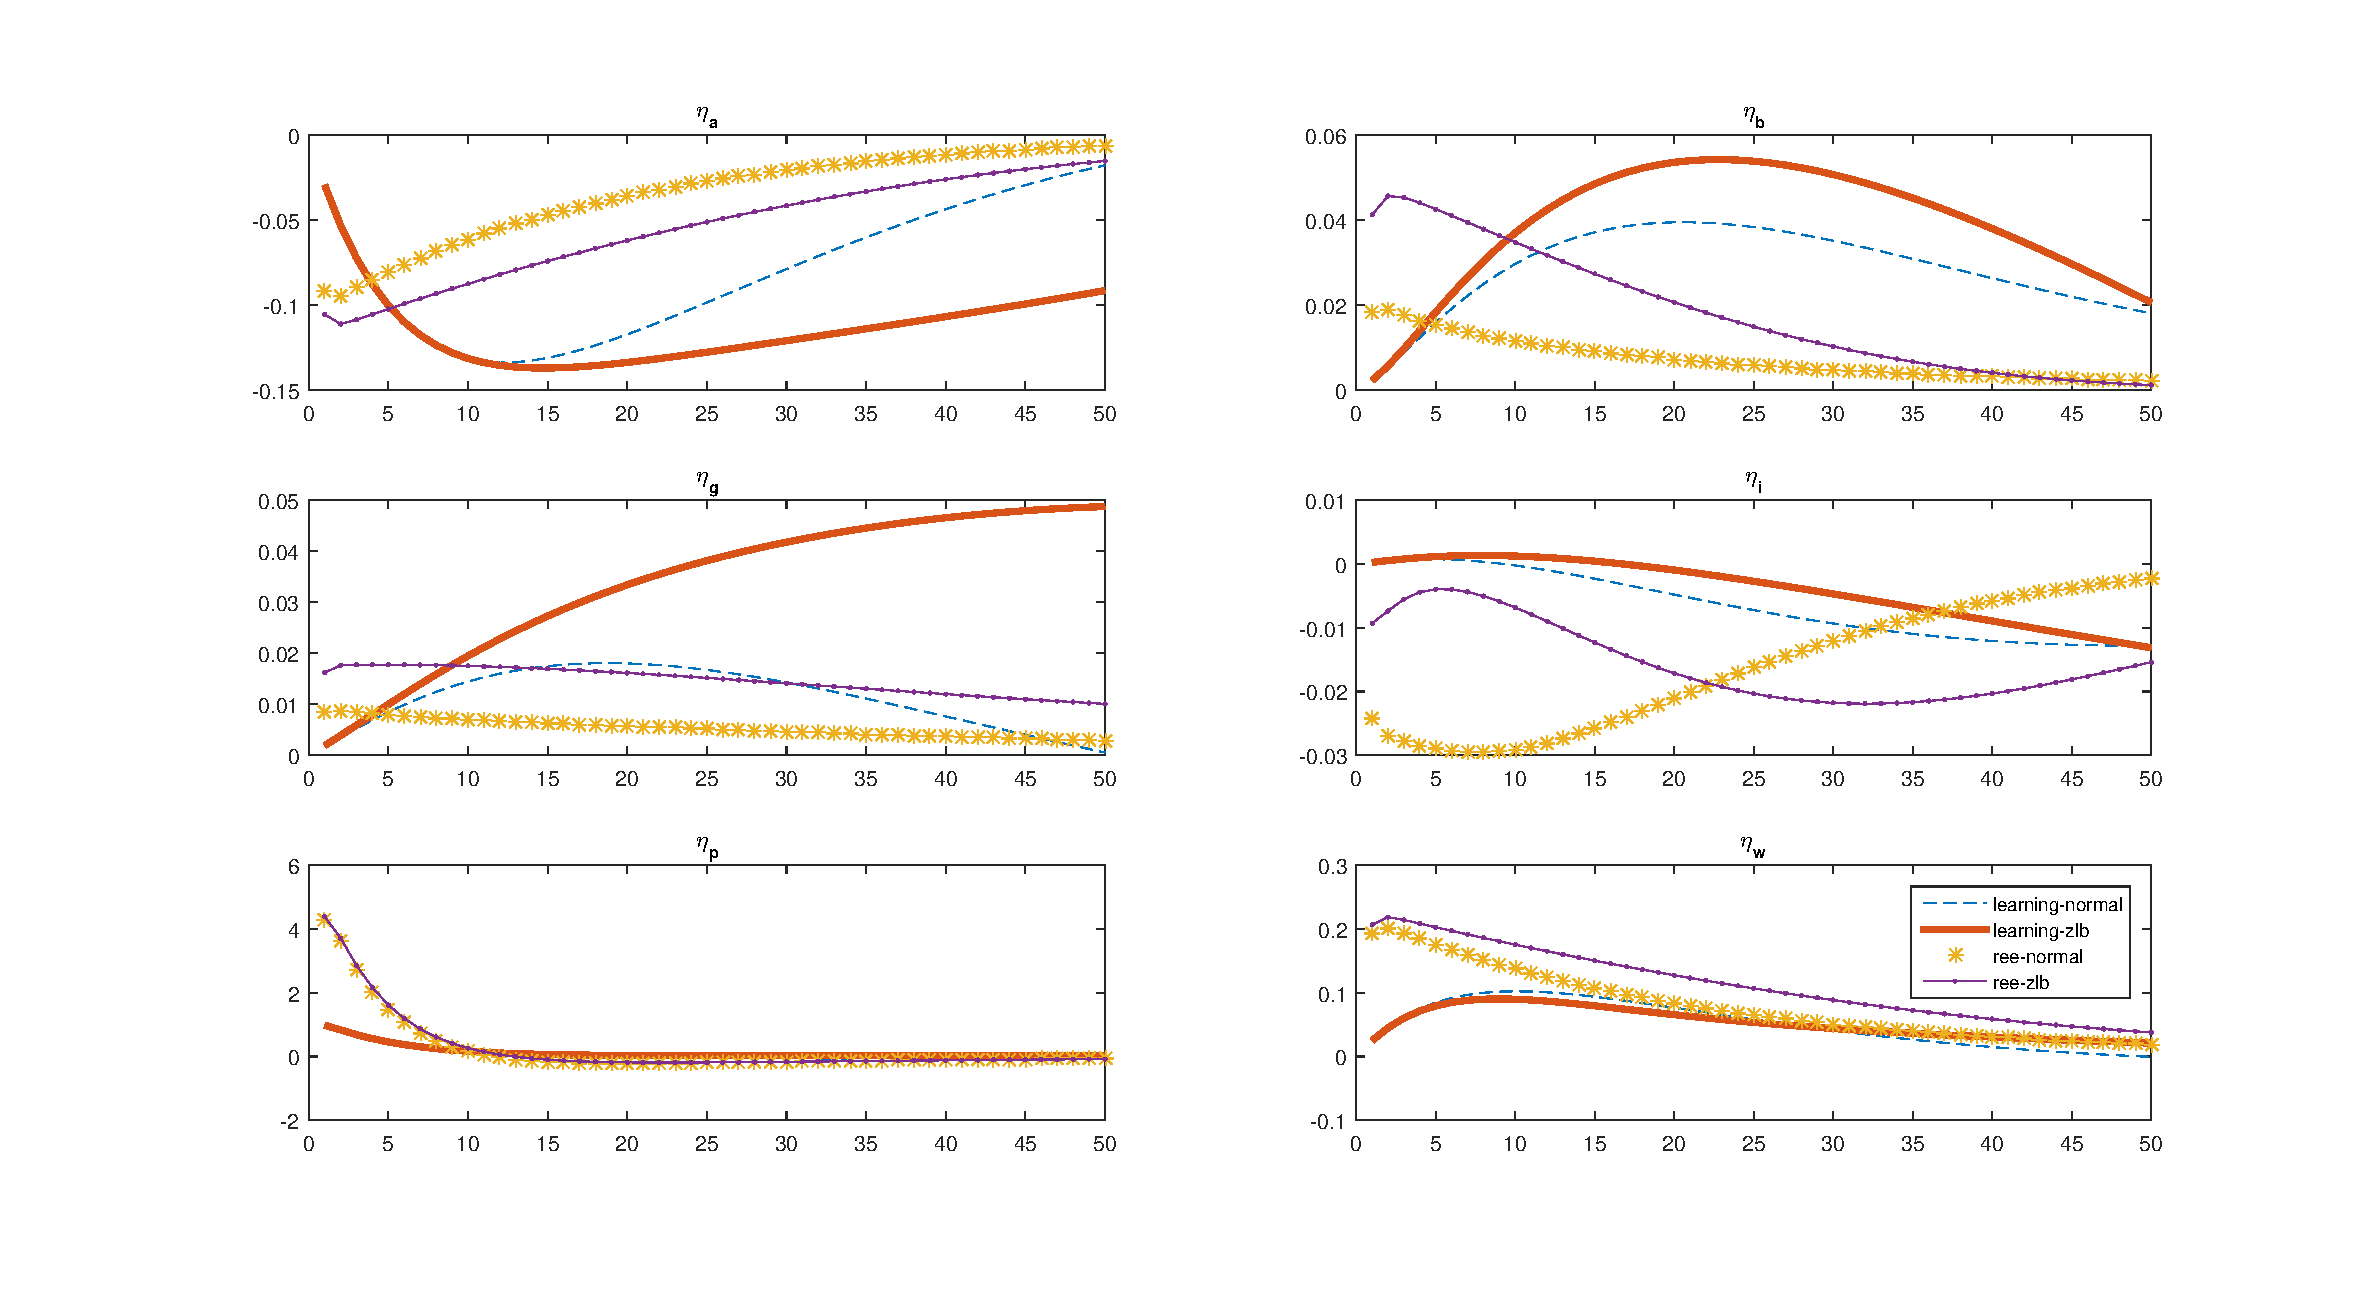
\includegraphics[scale=0.5]{AR1_impresp_pinf_riseComp.pdf}

\end{figure}


\begin{figure}[H]
\caption{Comparison of MSV learning IRFs with RISE IRFs. One unit shocks of $\eta_a$,$\eta_b$,$\eta_g$,$\eta_i$,$\eta_p$,$\eta_w$ respectively.}
\textbf{Consumption:}\\
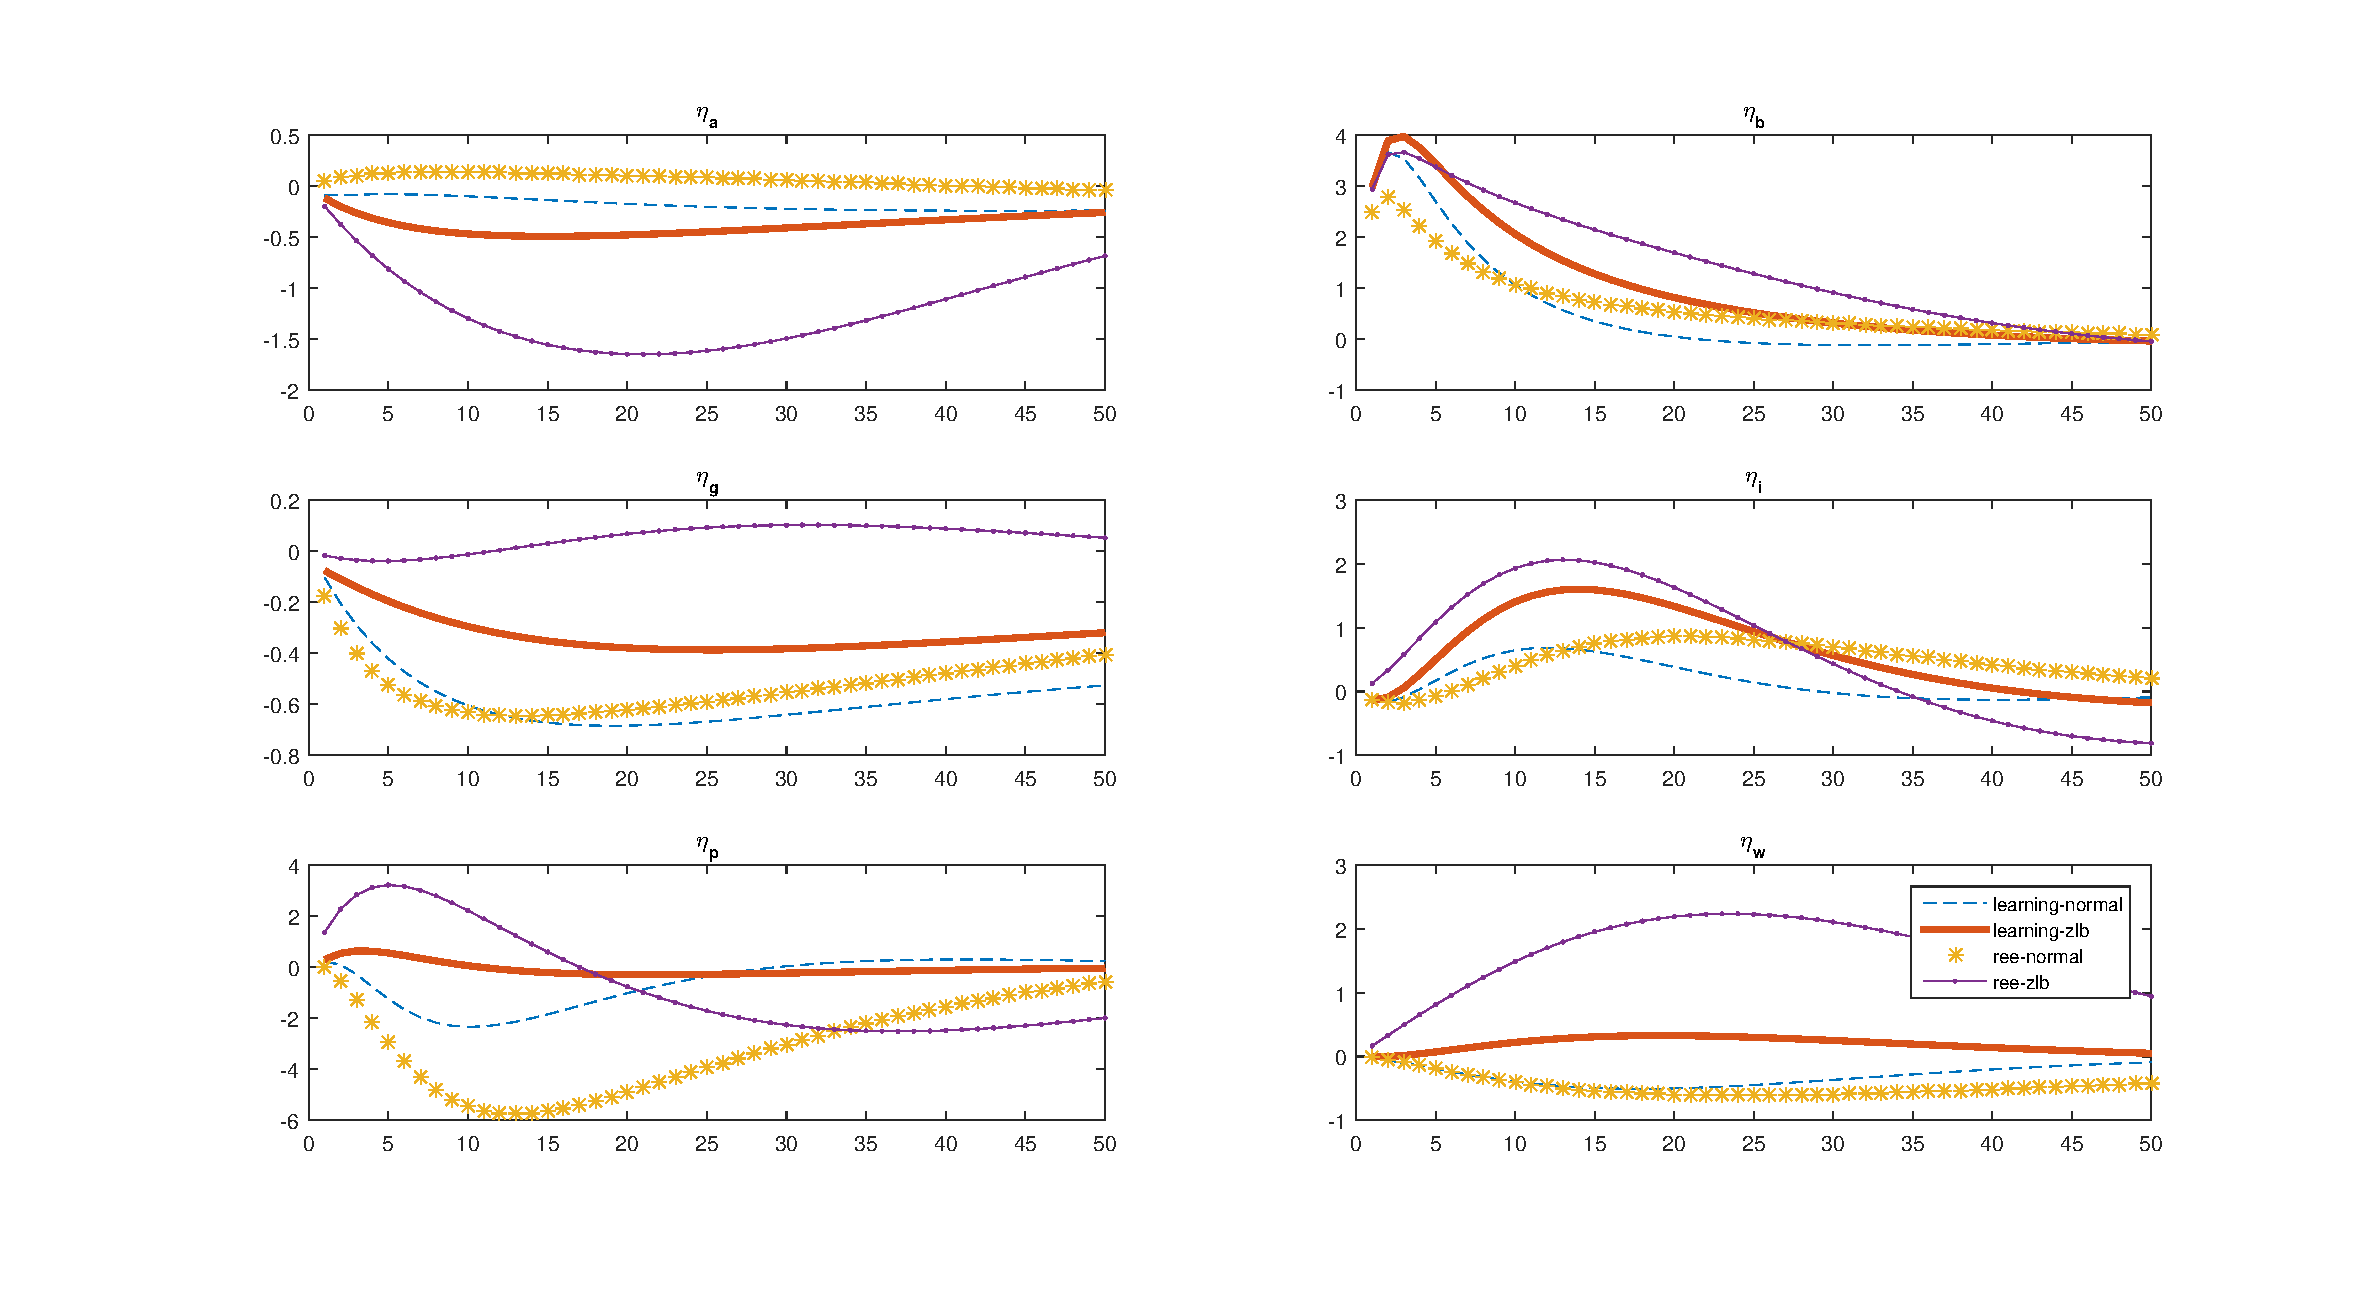
\includegraphics[scale=0.5]{MSV_impresp_cons_riseComp.pdf}
\textbf{Investment:}\\
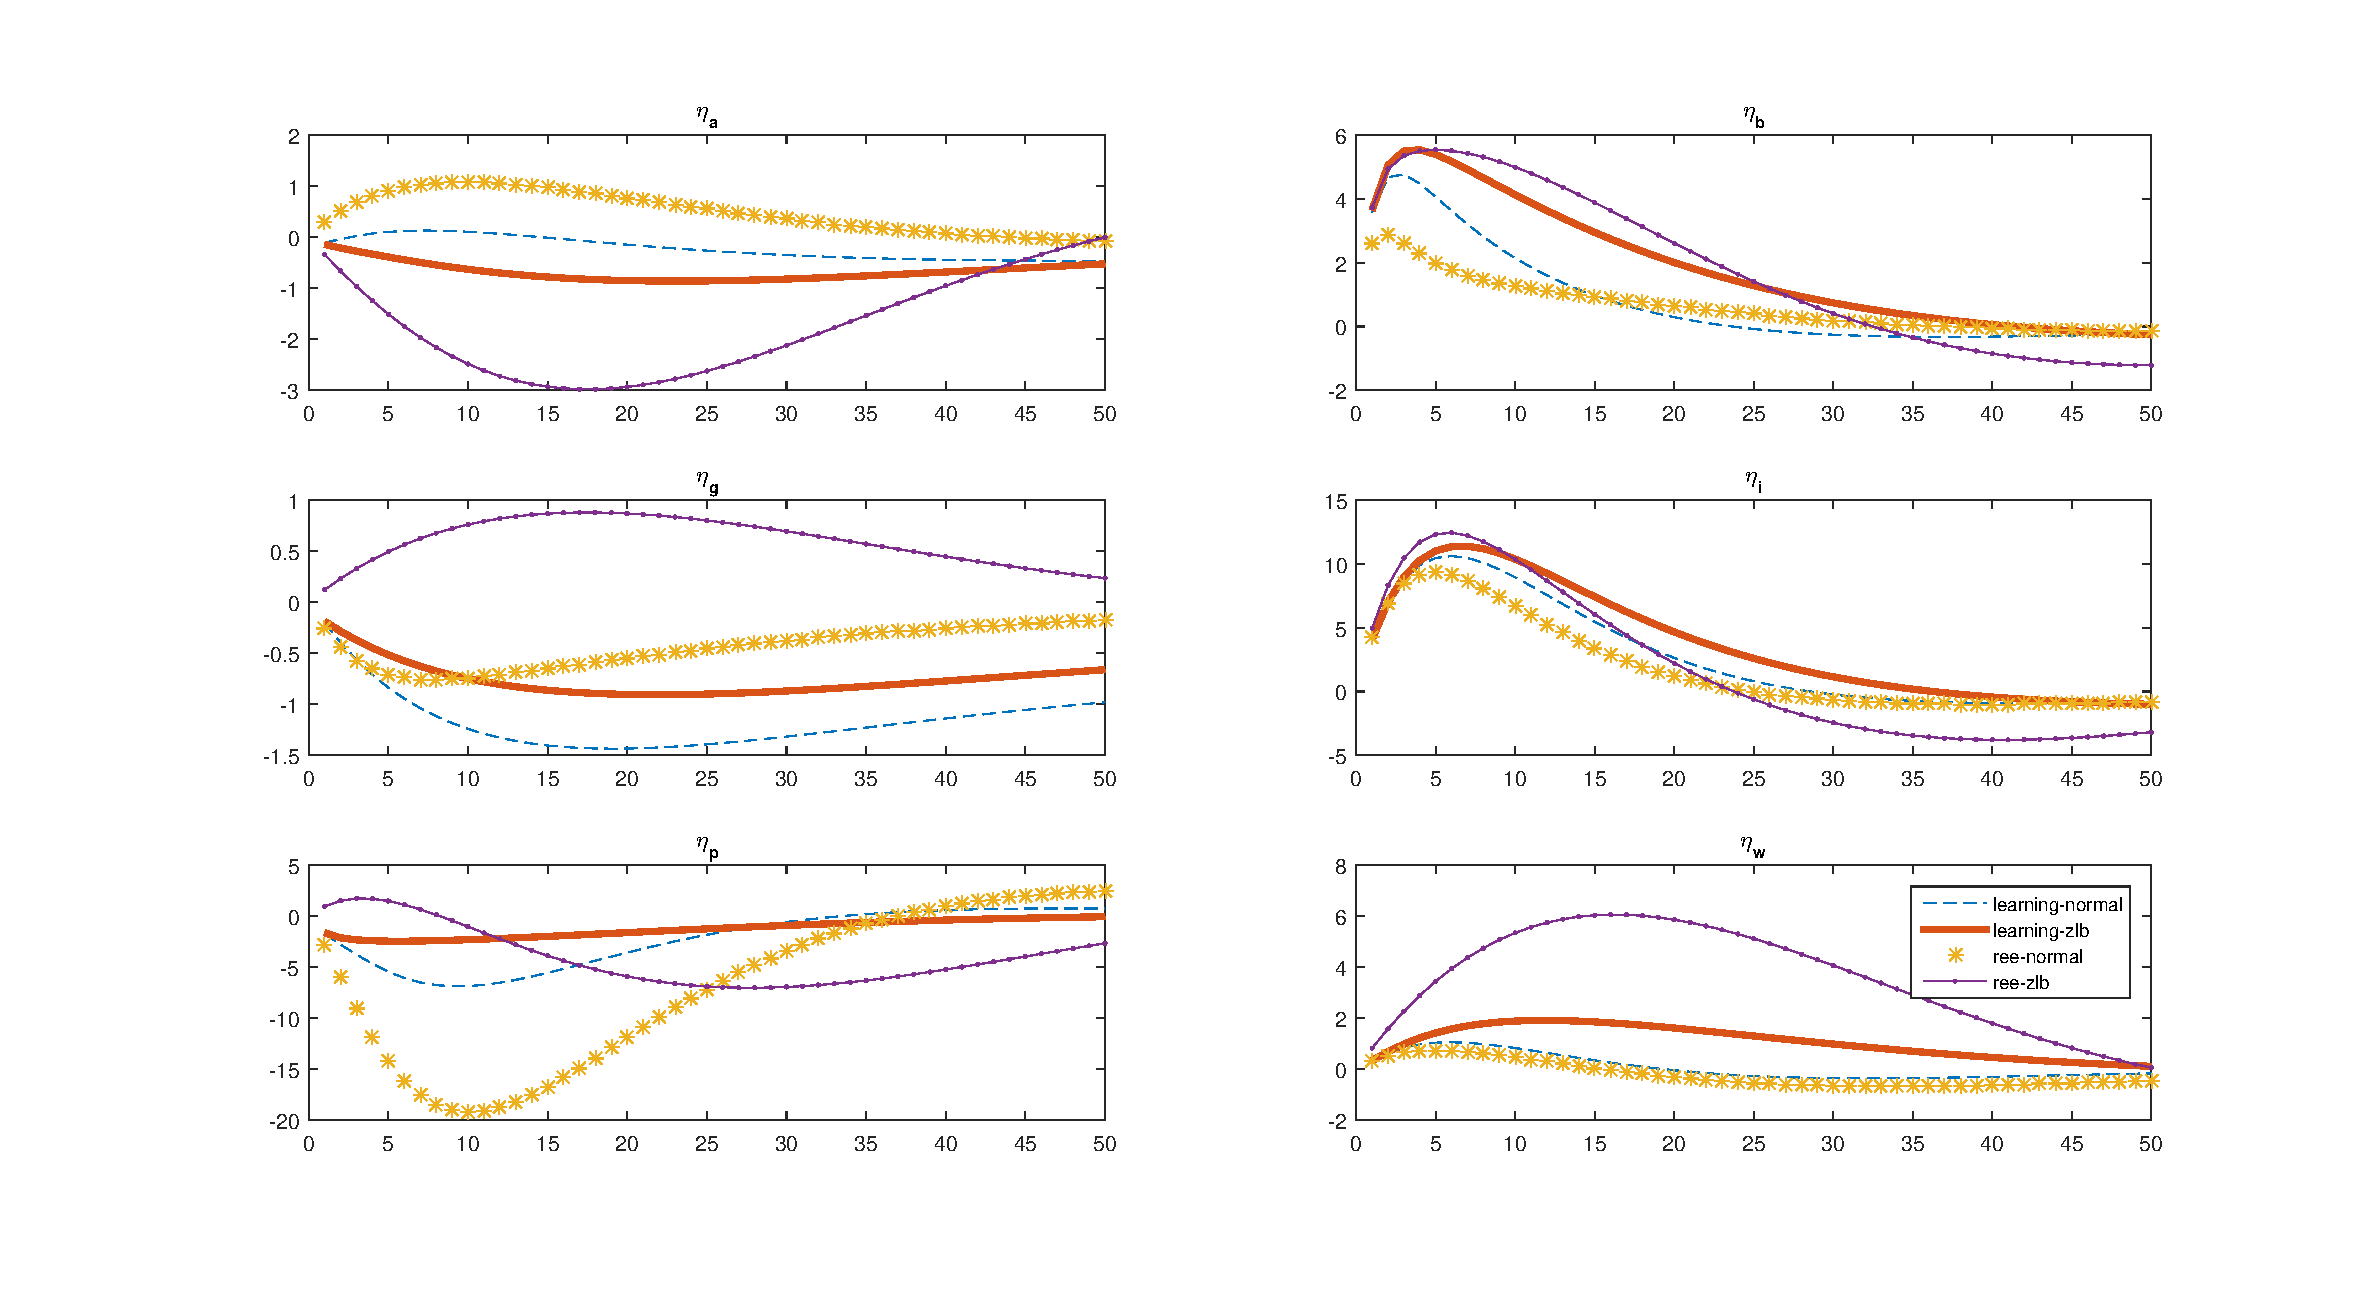
\includegraphics[scale=0.5]{MSV_impresp_inv_riseComp.pdf}

\end{figure}

\begin{figure}[H]
\textbf{Output:}\\
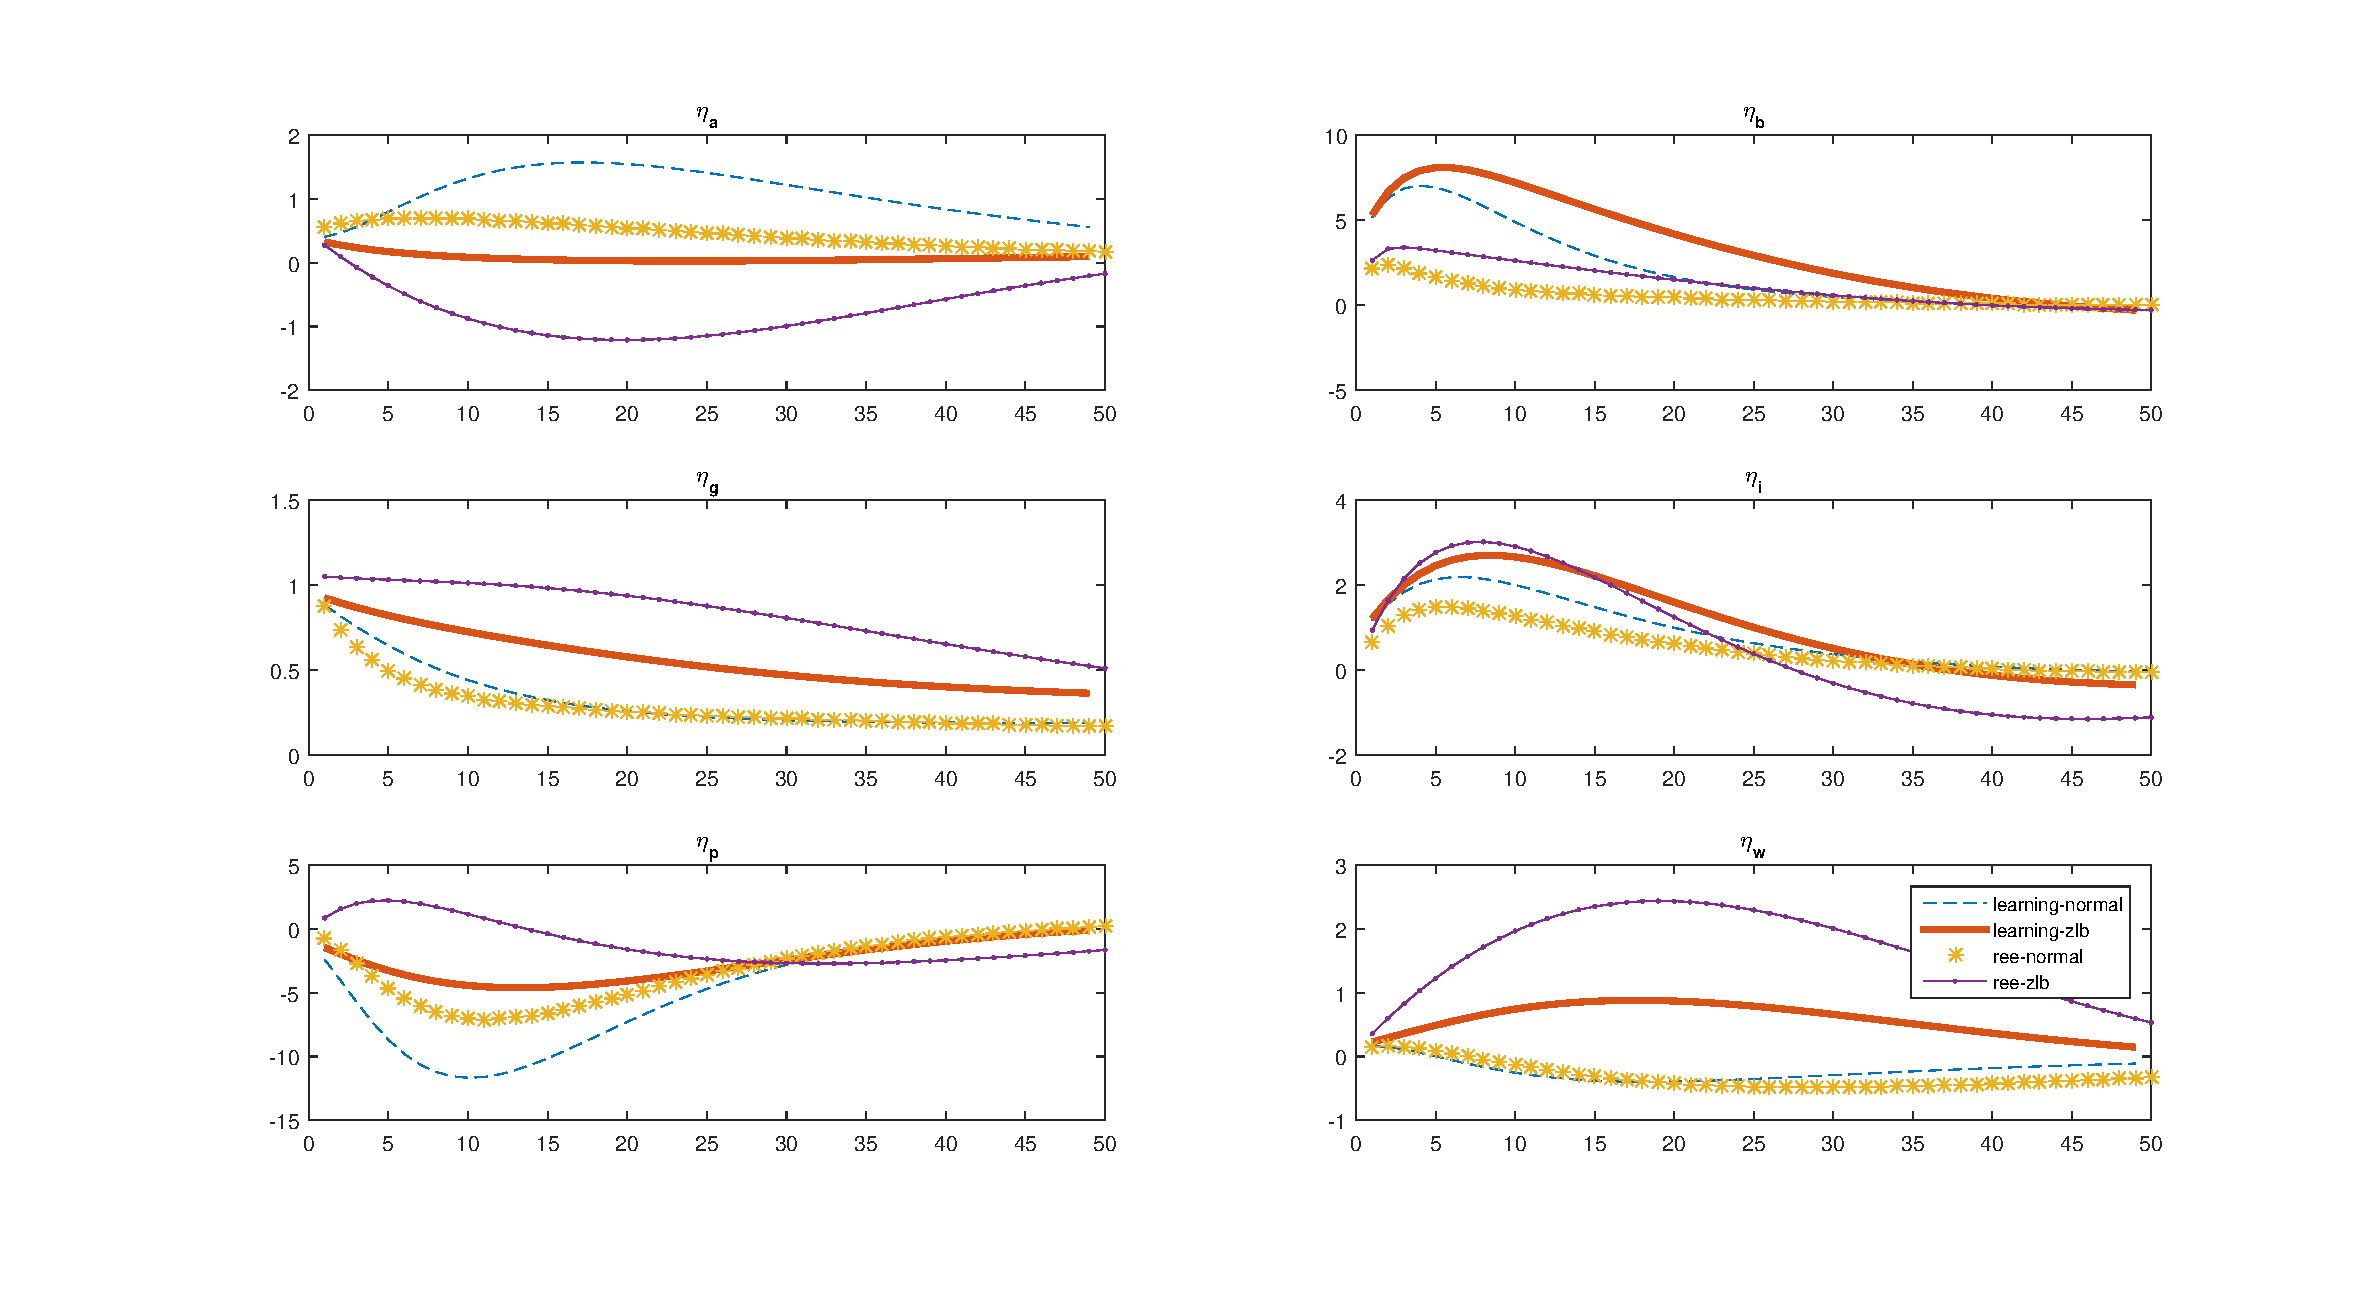
\includegraphics[scale=0.5]{MSV_impresp_output_riseComp.pdf}
\textbf{Inflation:}\\
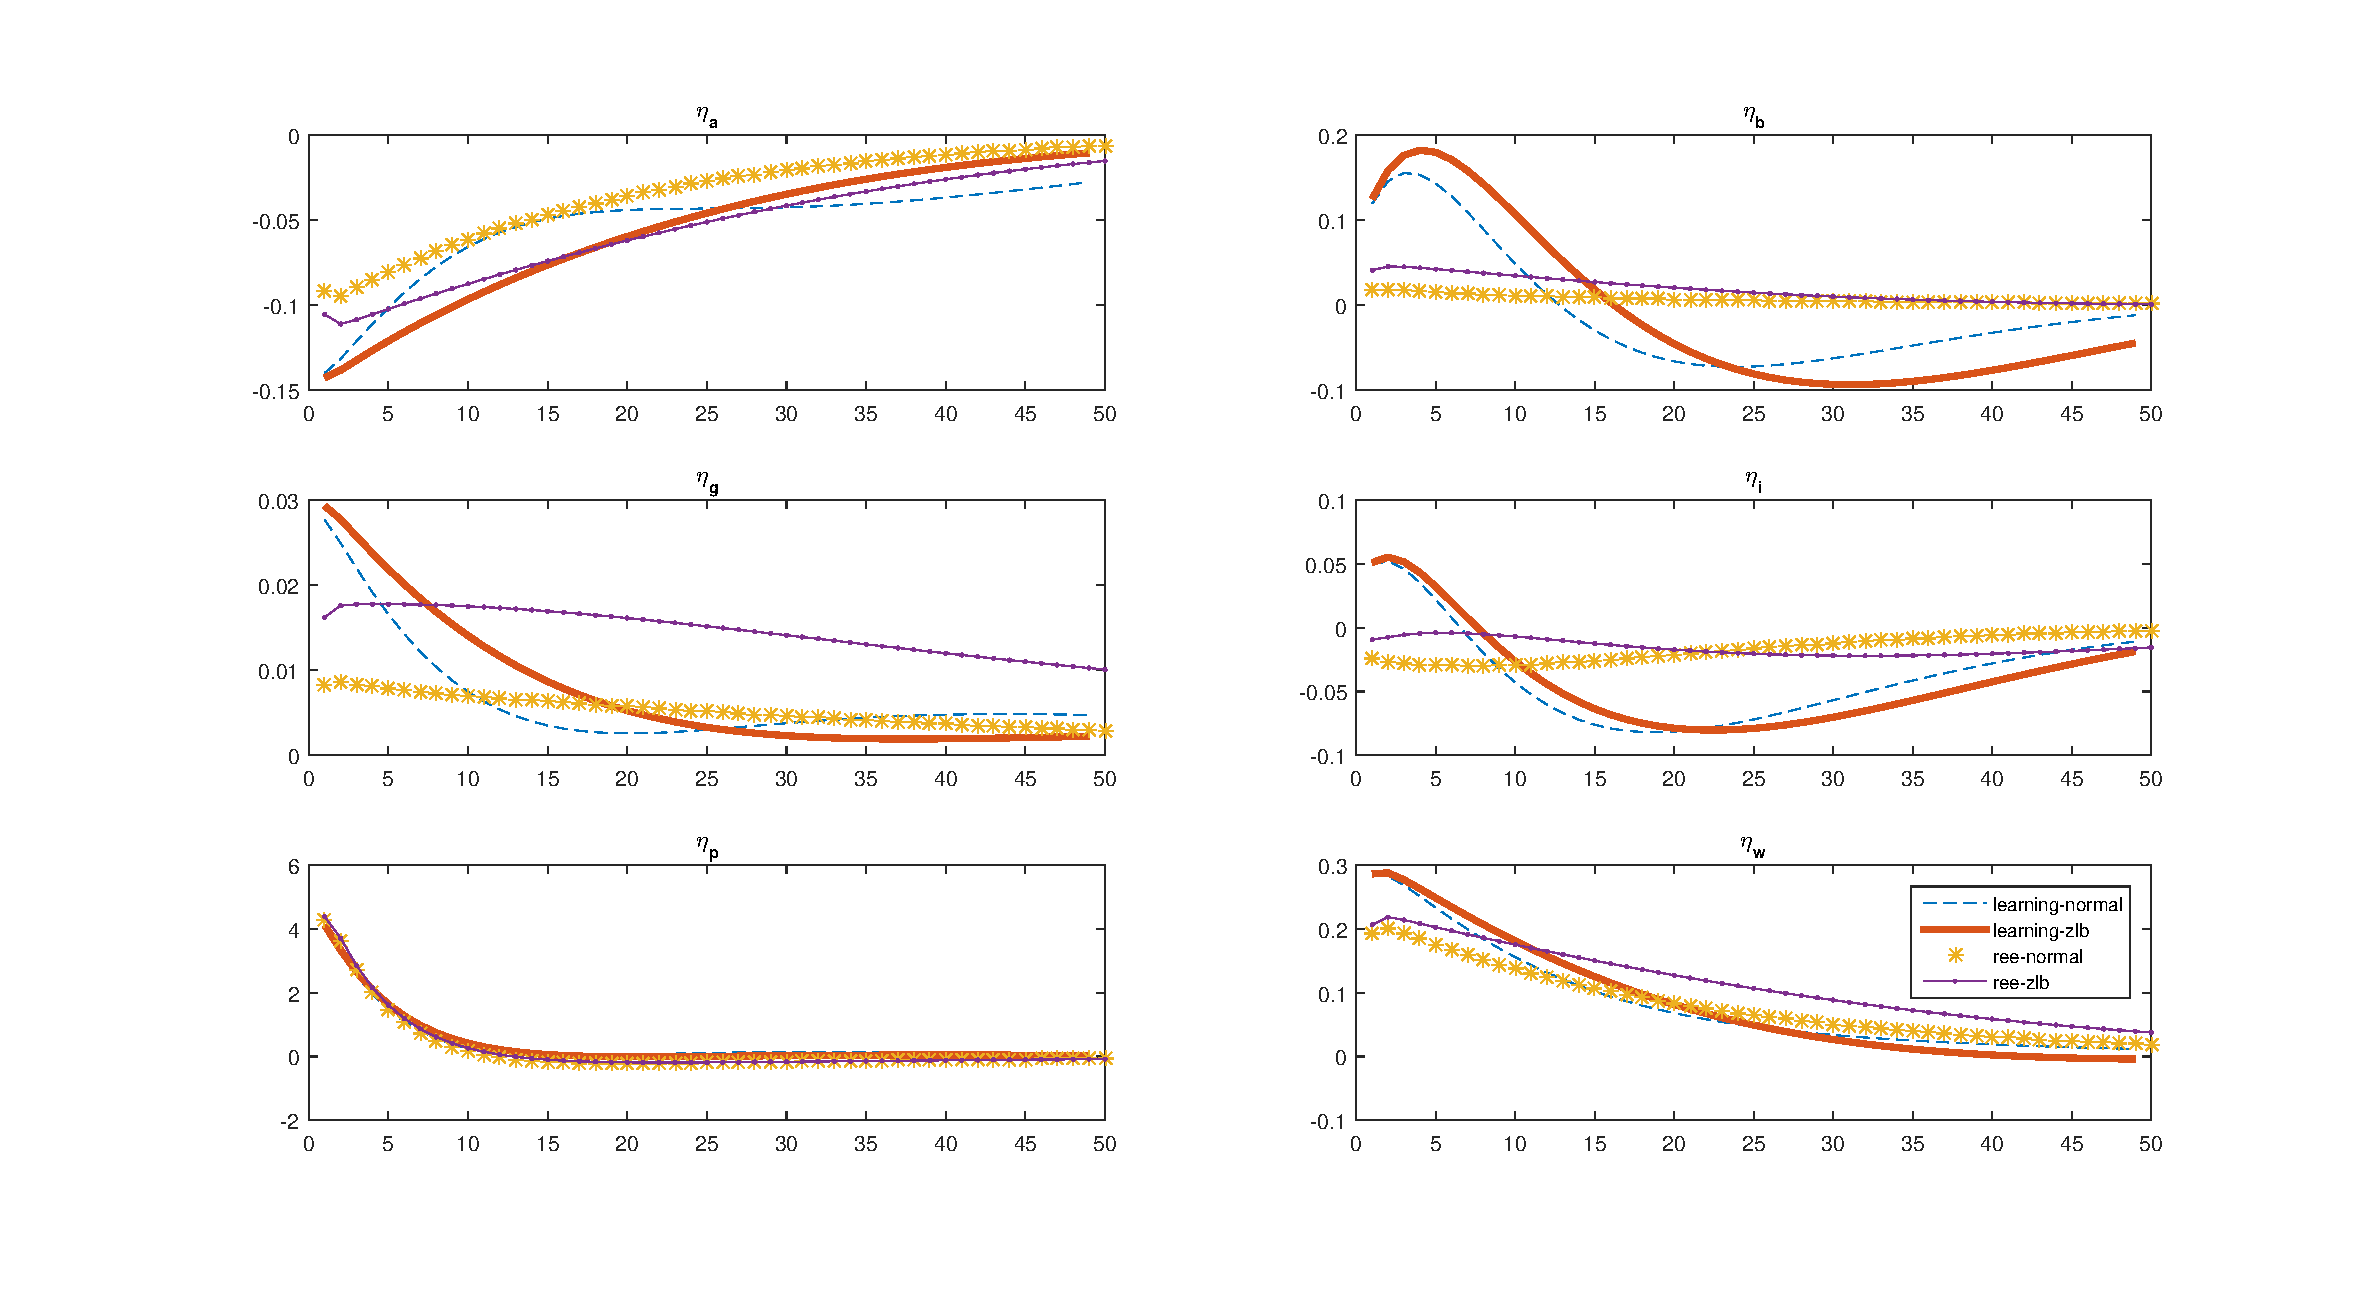
\includegraphics[scale=0.5]{MSV_impresp_pinf_riseComp.pdf}

\end{figure}






\begin{figure}[H]
\textbf{Consumption:}\\
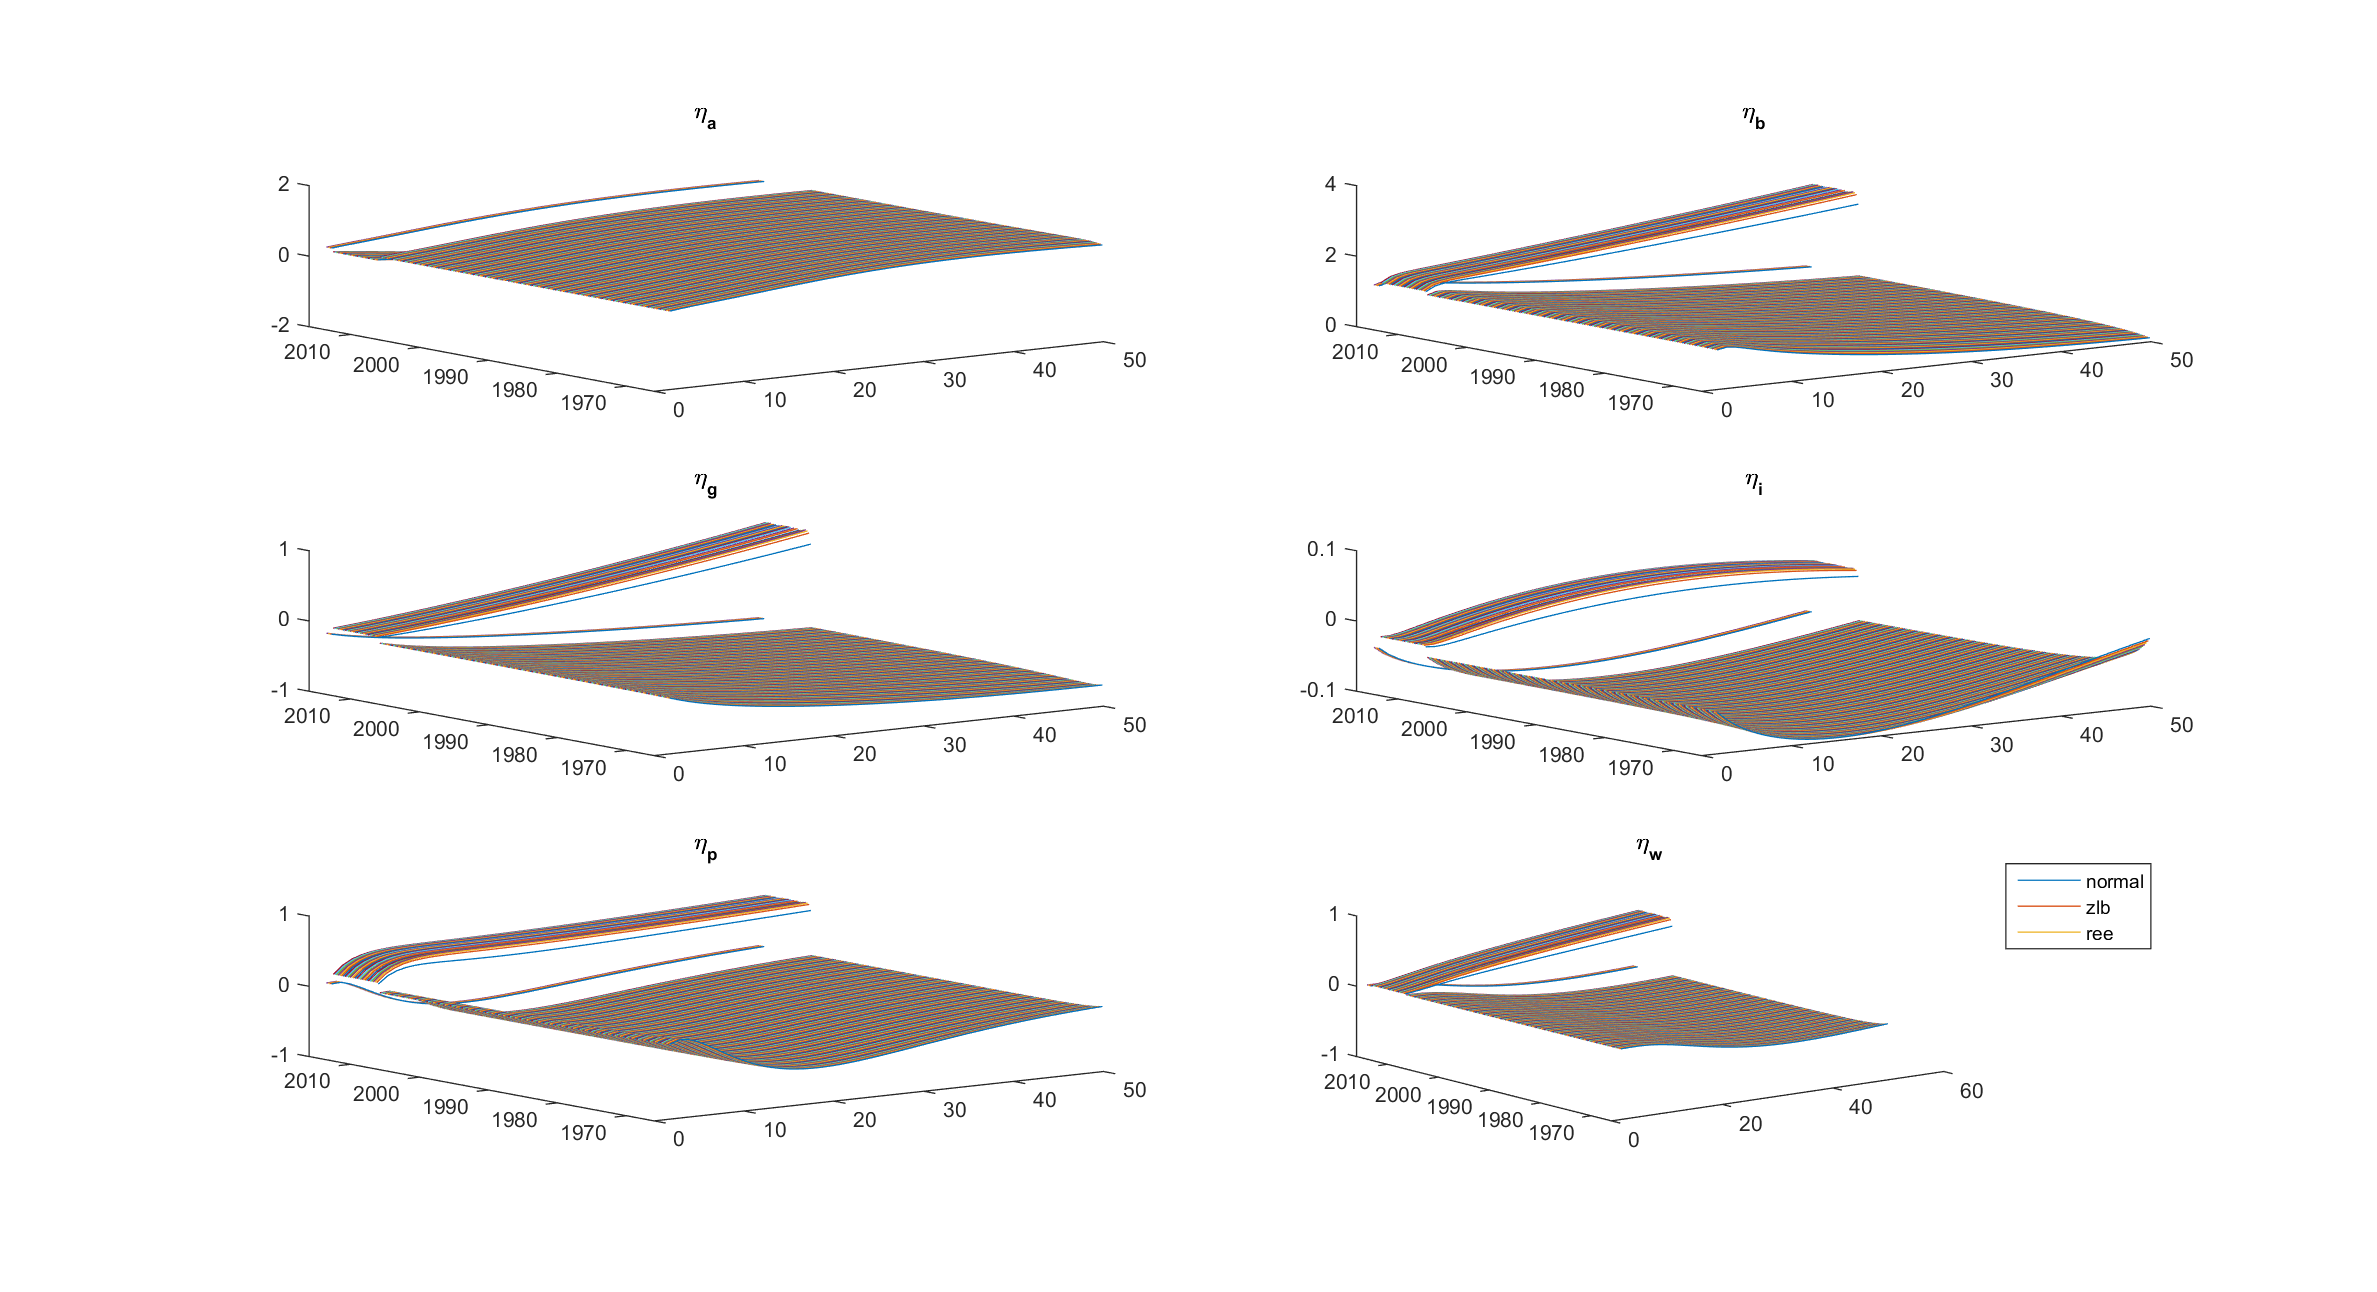
\includegraphics[scale=0.5]{AR1_impresp_cons_3d.pdf}
\textbf{Investment:}\\
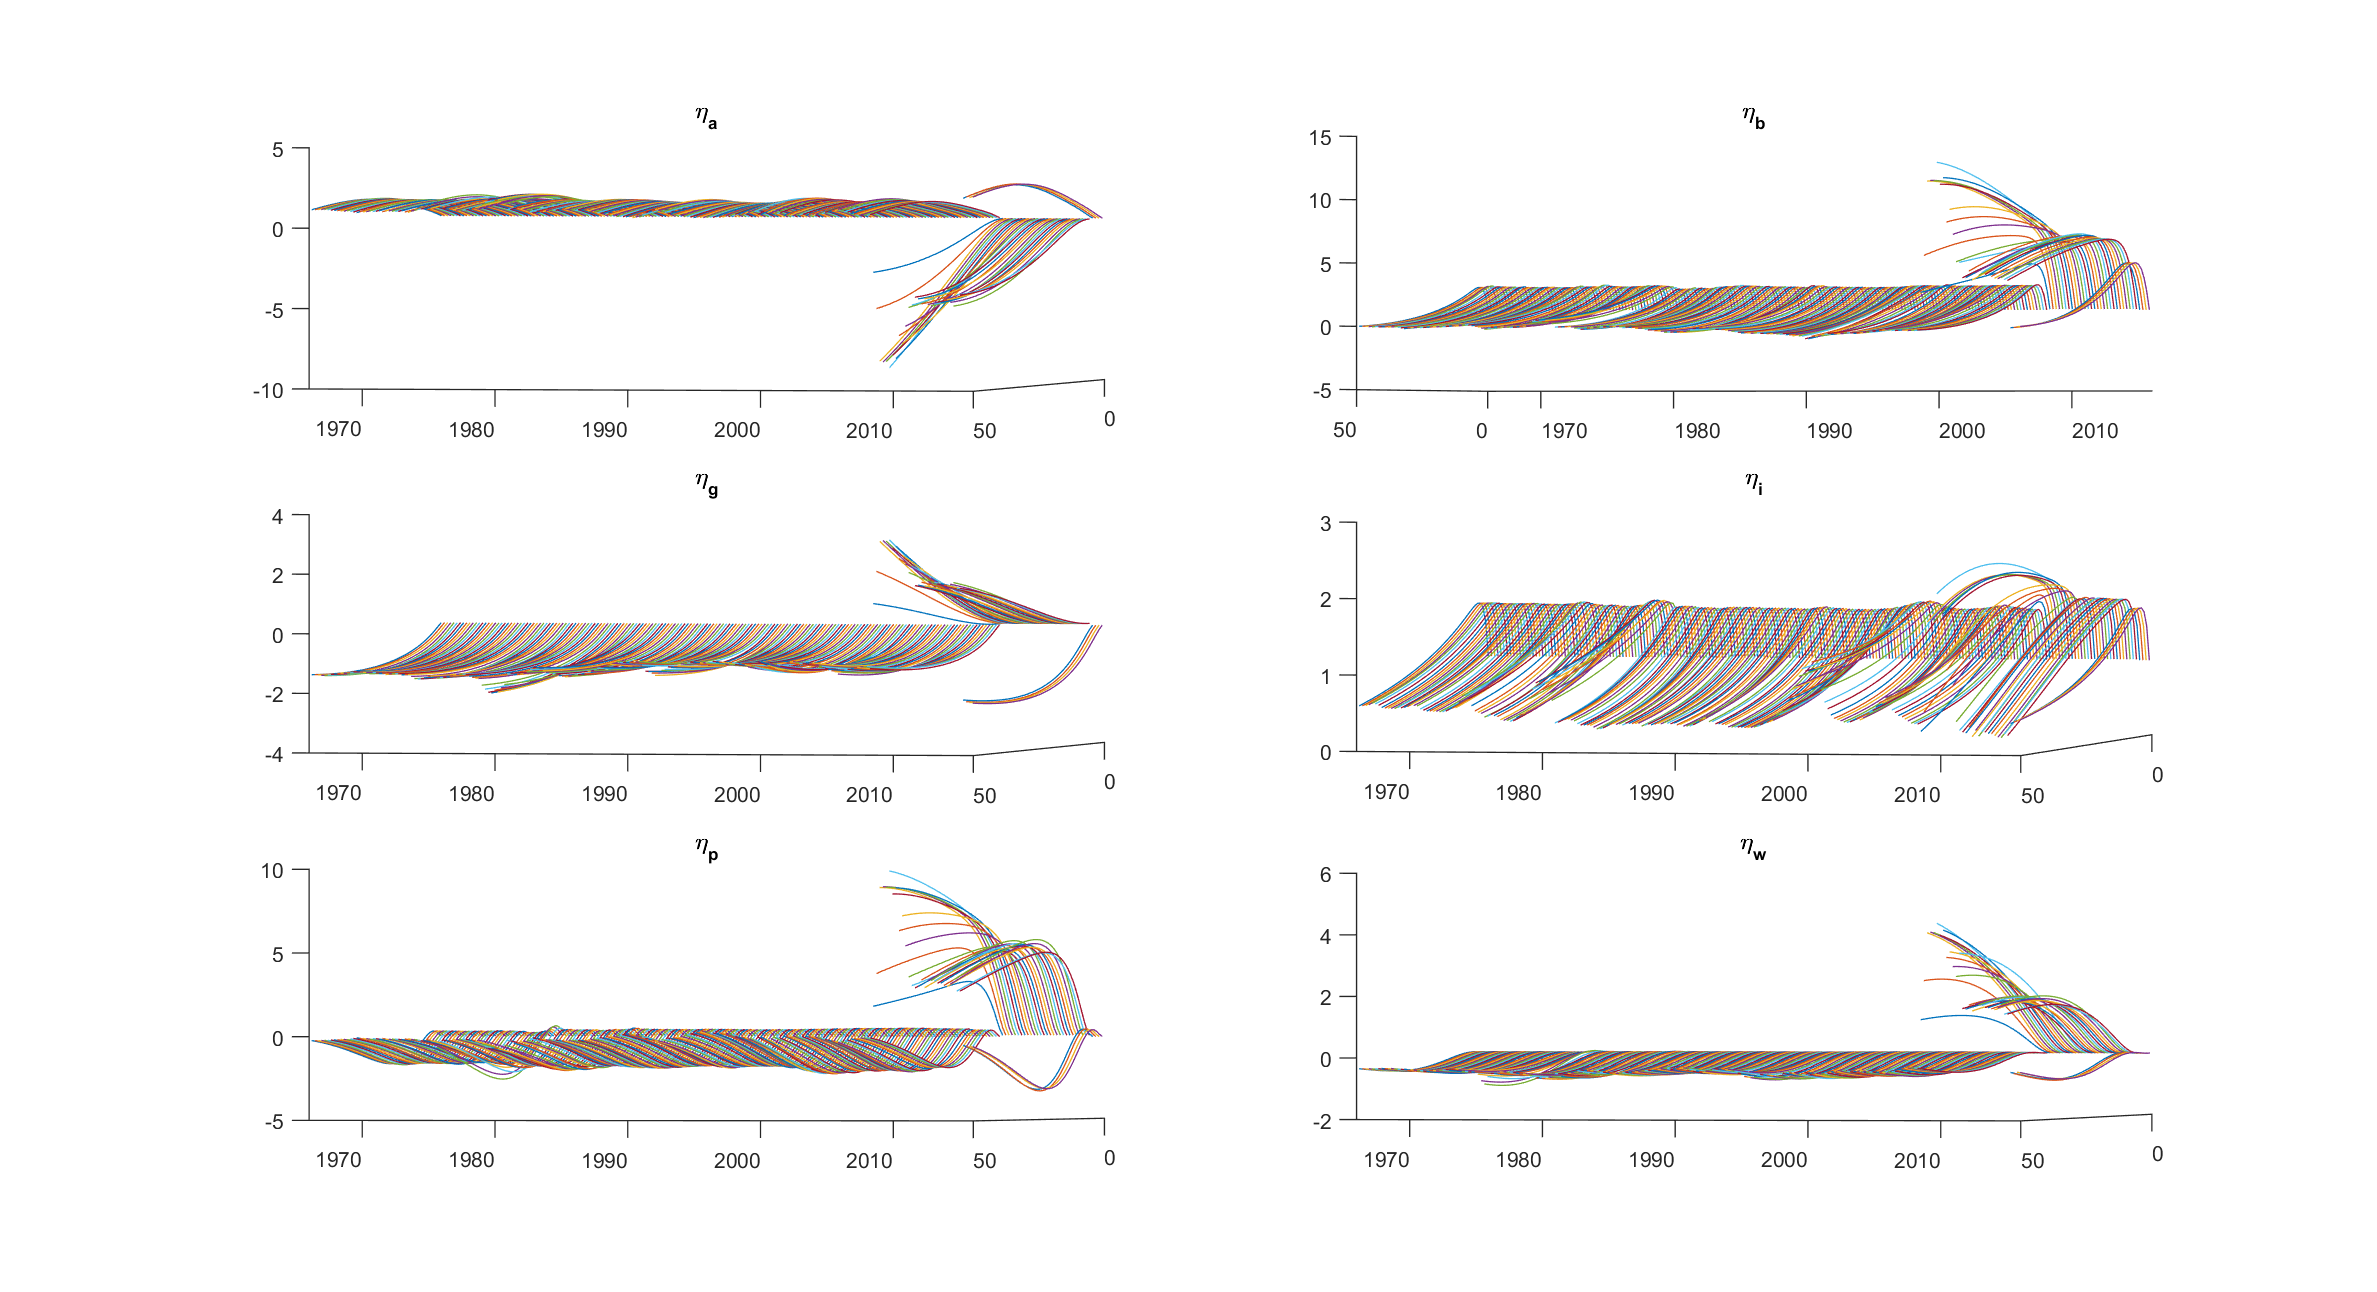
\includegraphics[scale=0.5]{AR1_impresp_inv_3d.pdf}

\end{figure}

\begin{figure}[H]
\textbf{Output:}\\
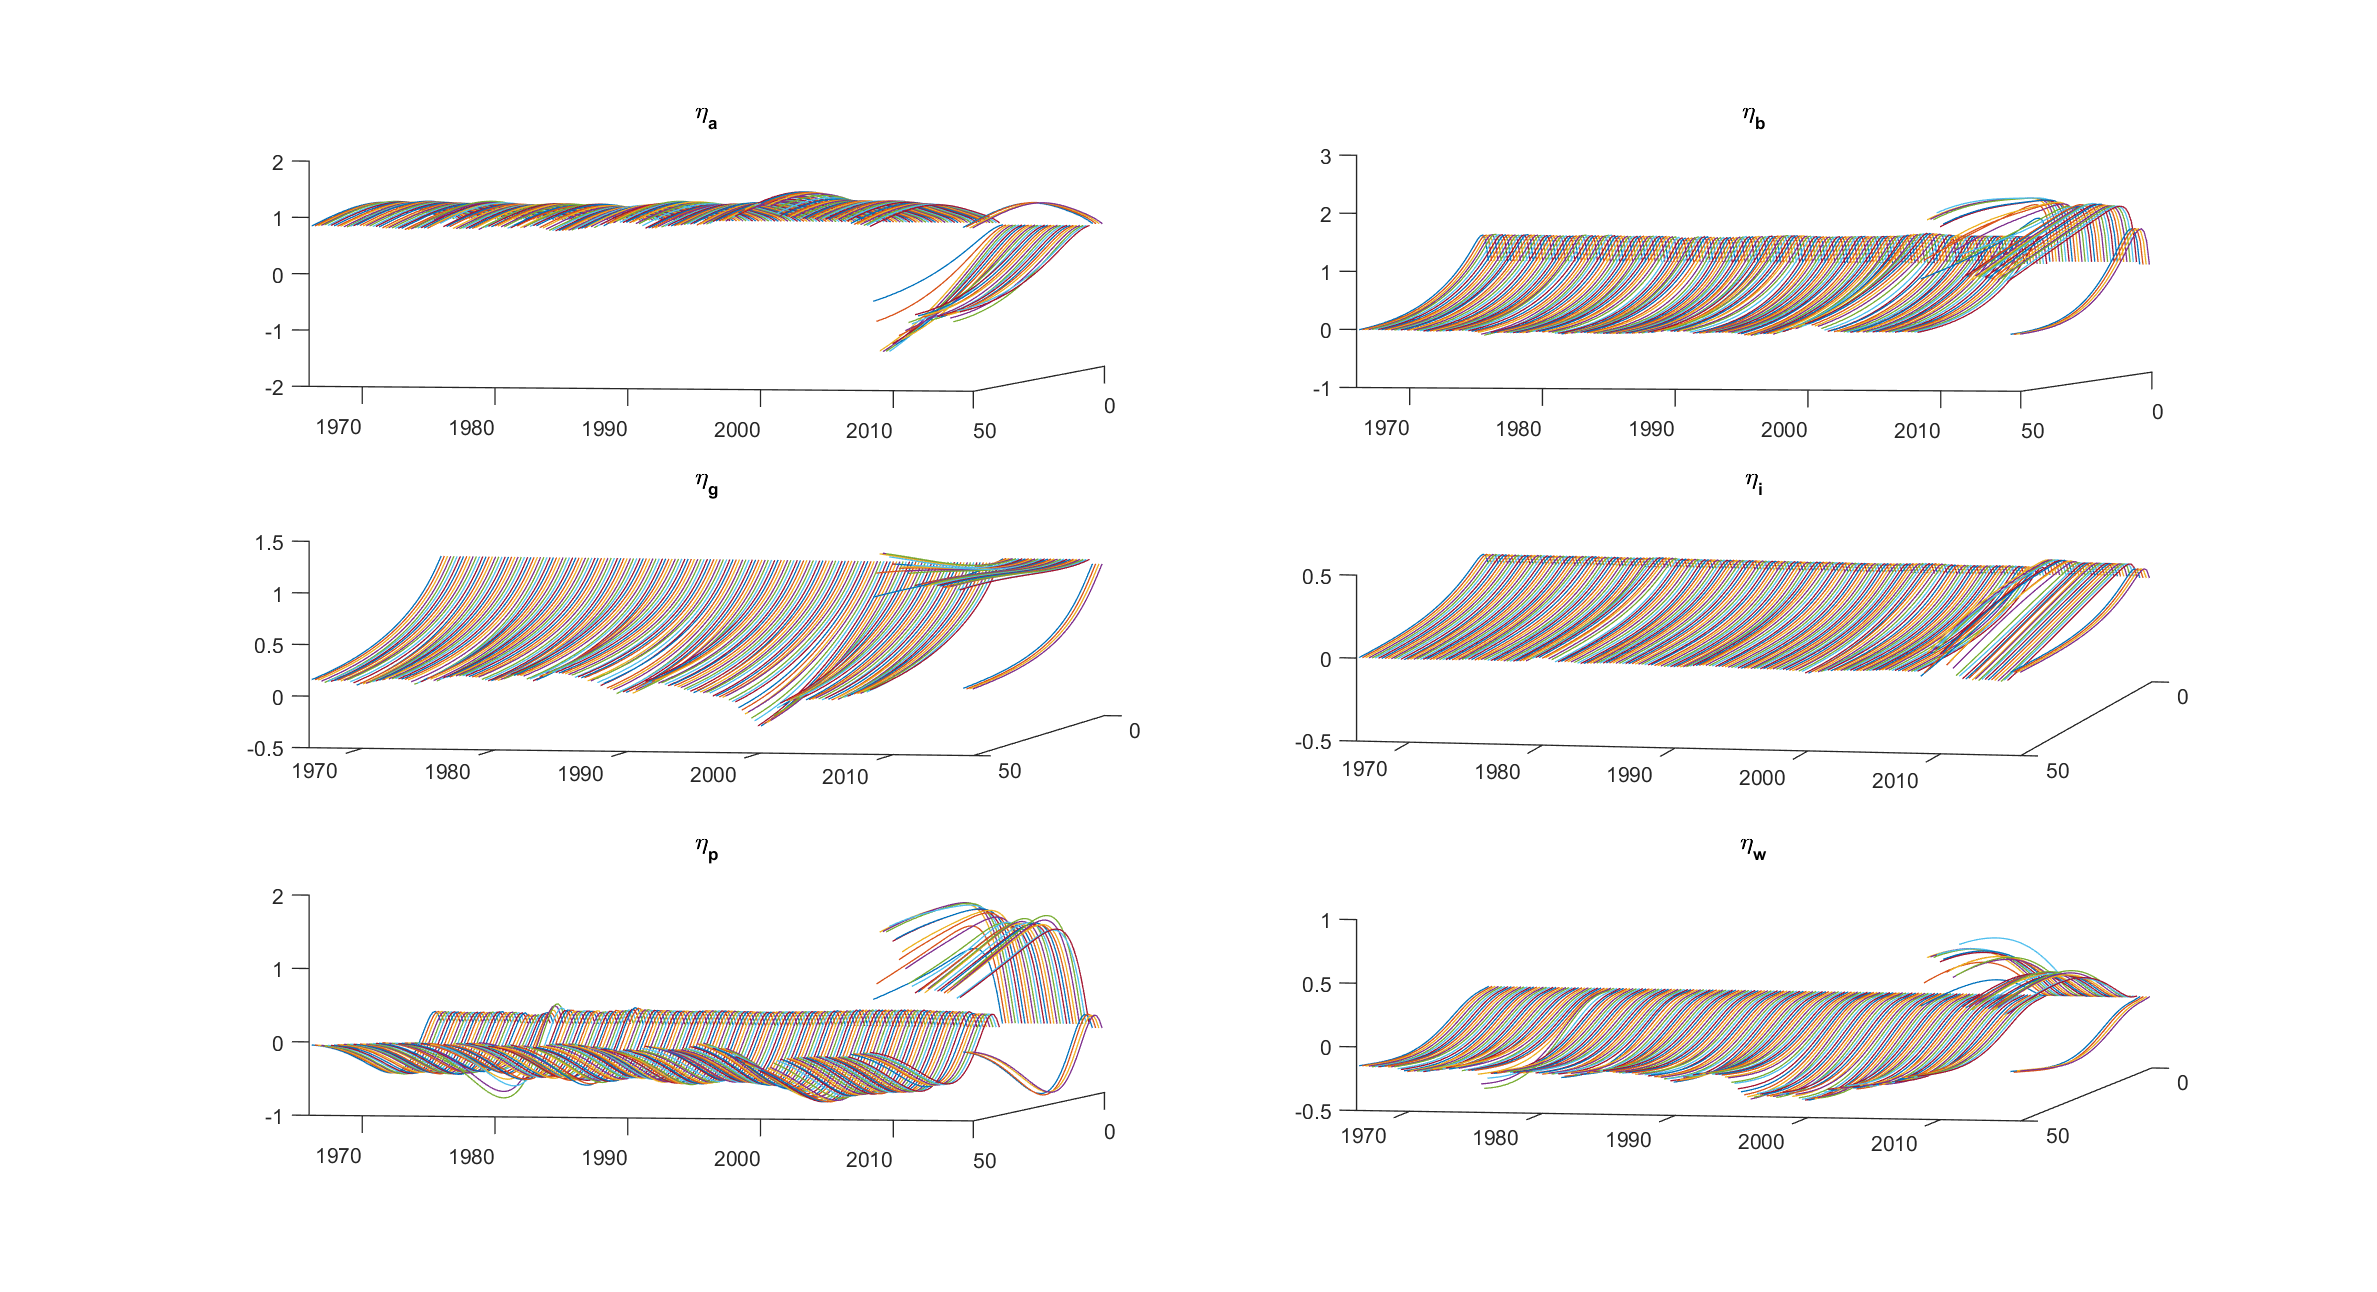
\includegraphics[scale=0.5]{AR1_impresp_output_3d.pdf}
\textbf{Inflation:}\\
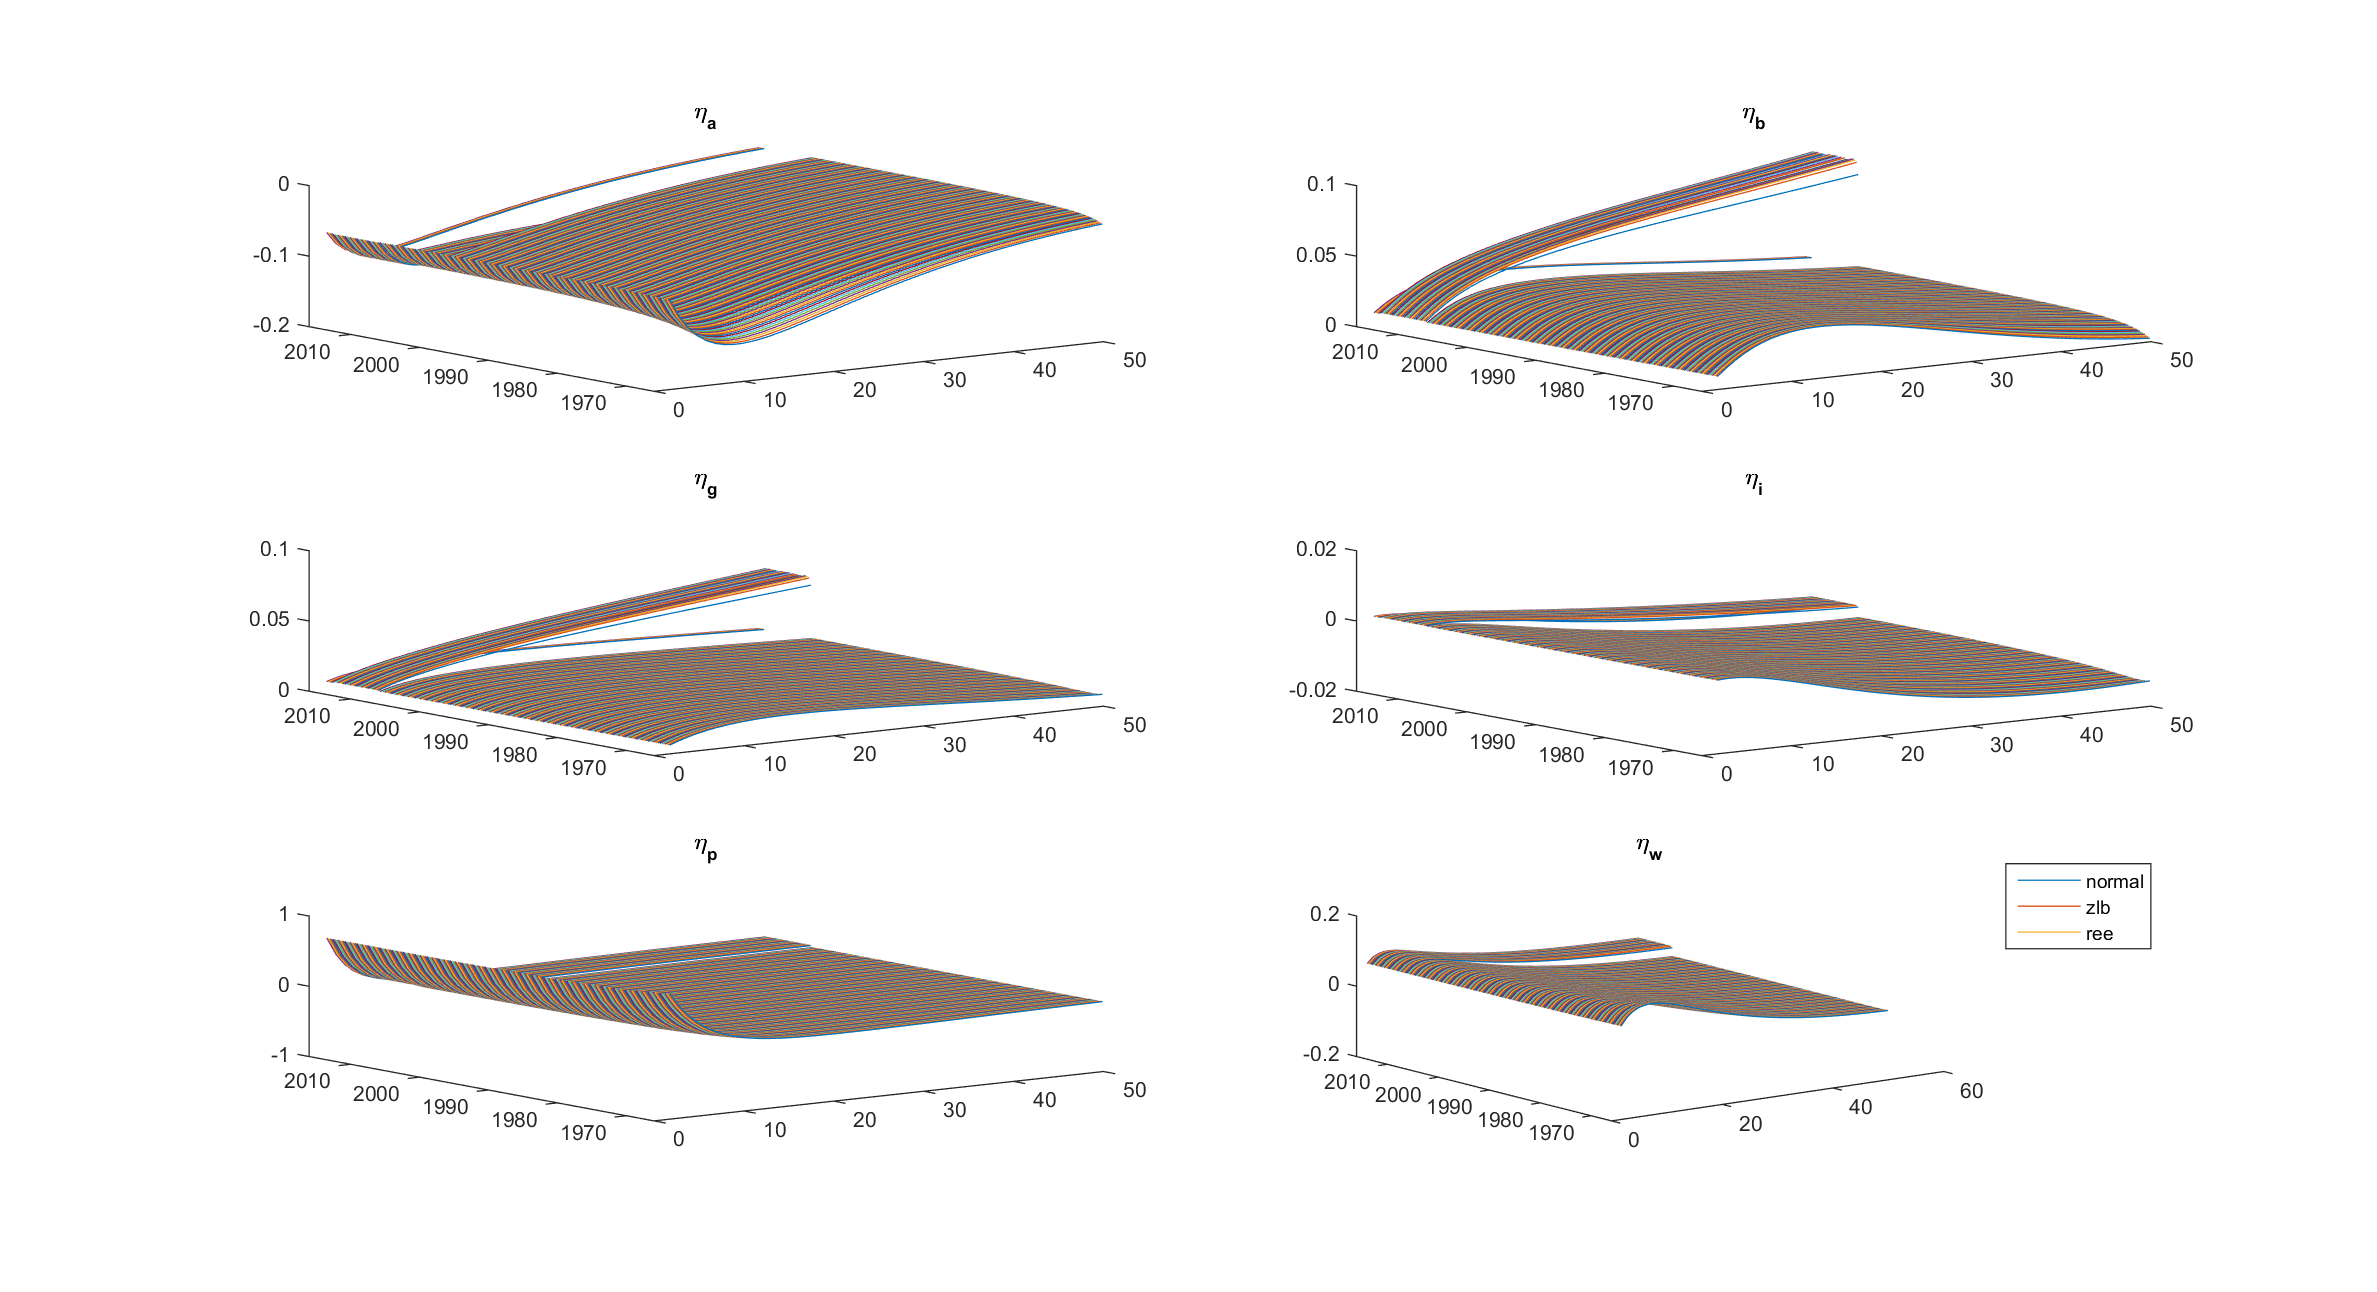
\includegraphics[scale=0.5]{AR1_impresp_pinf_3d.pdf}

\end{figure}




\begin{figure}[H]
\textbf{Consumption:}\\
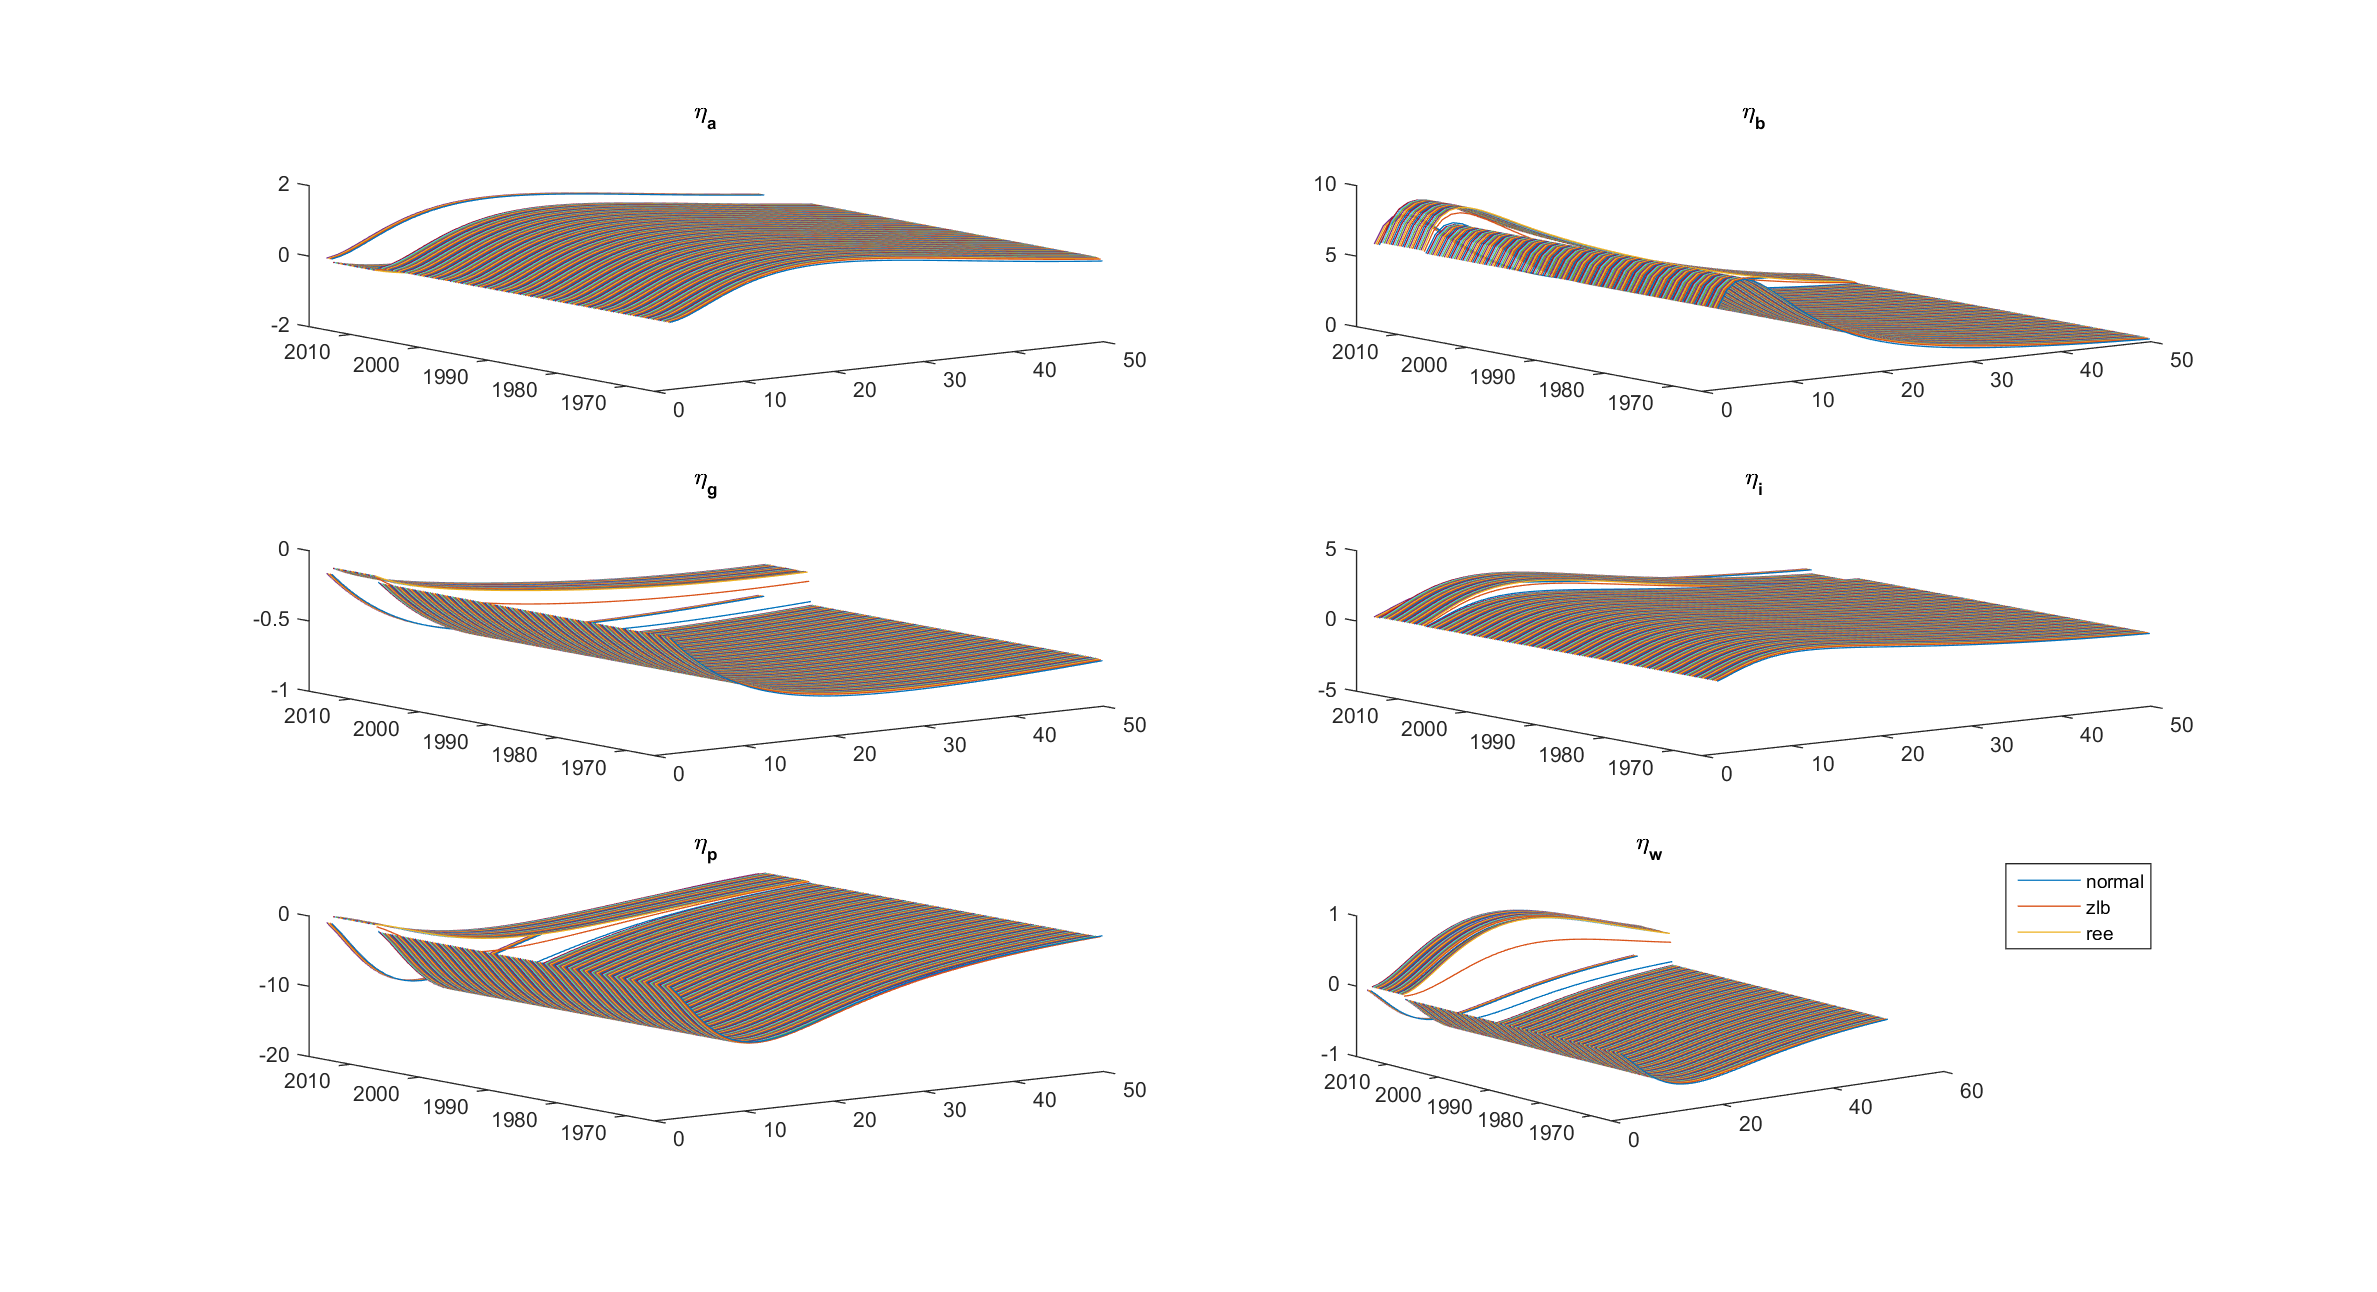
\includegraphics[scale=0.5]{MSV_impresp_cons_3d.pdf}
\textbf{Investment:}\\
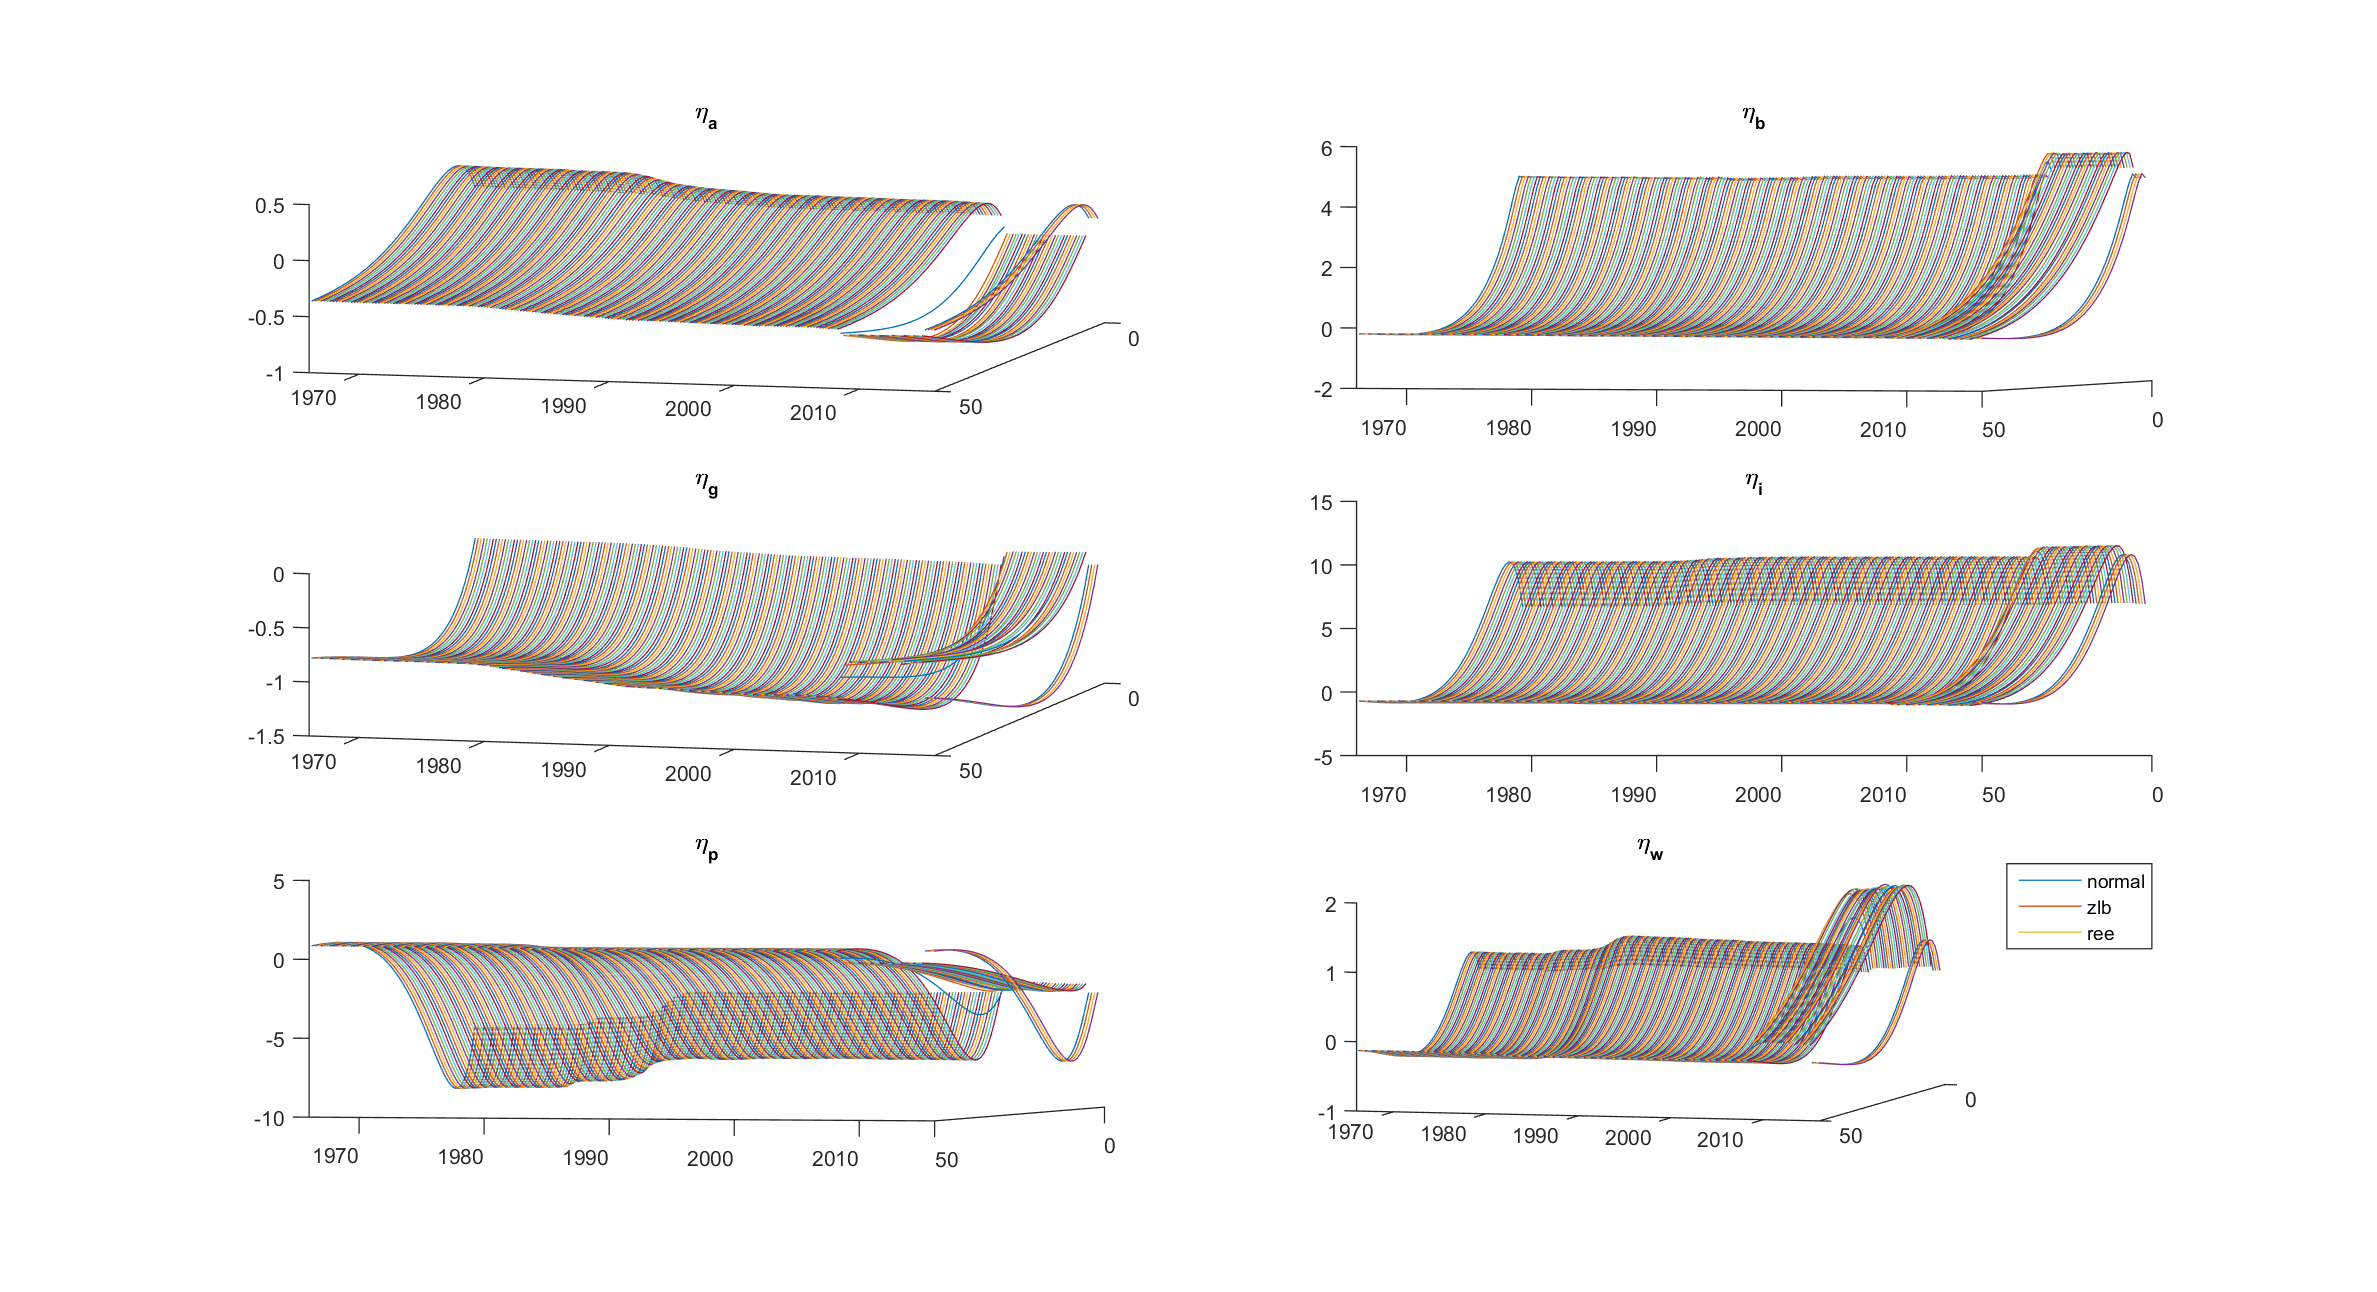
\includegraphics[scale=0.5]{MSV_impresp_inv_3d.pdf}

\end{figure}

\begin{figure}[H]
\textbf{Output:}\\
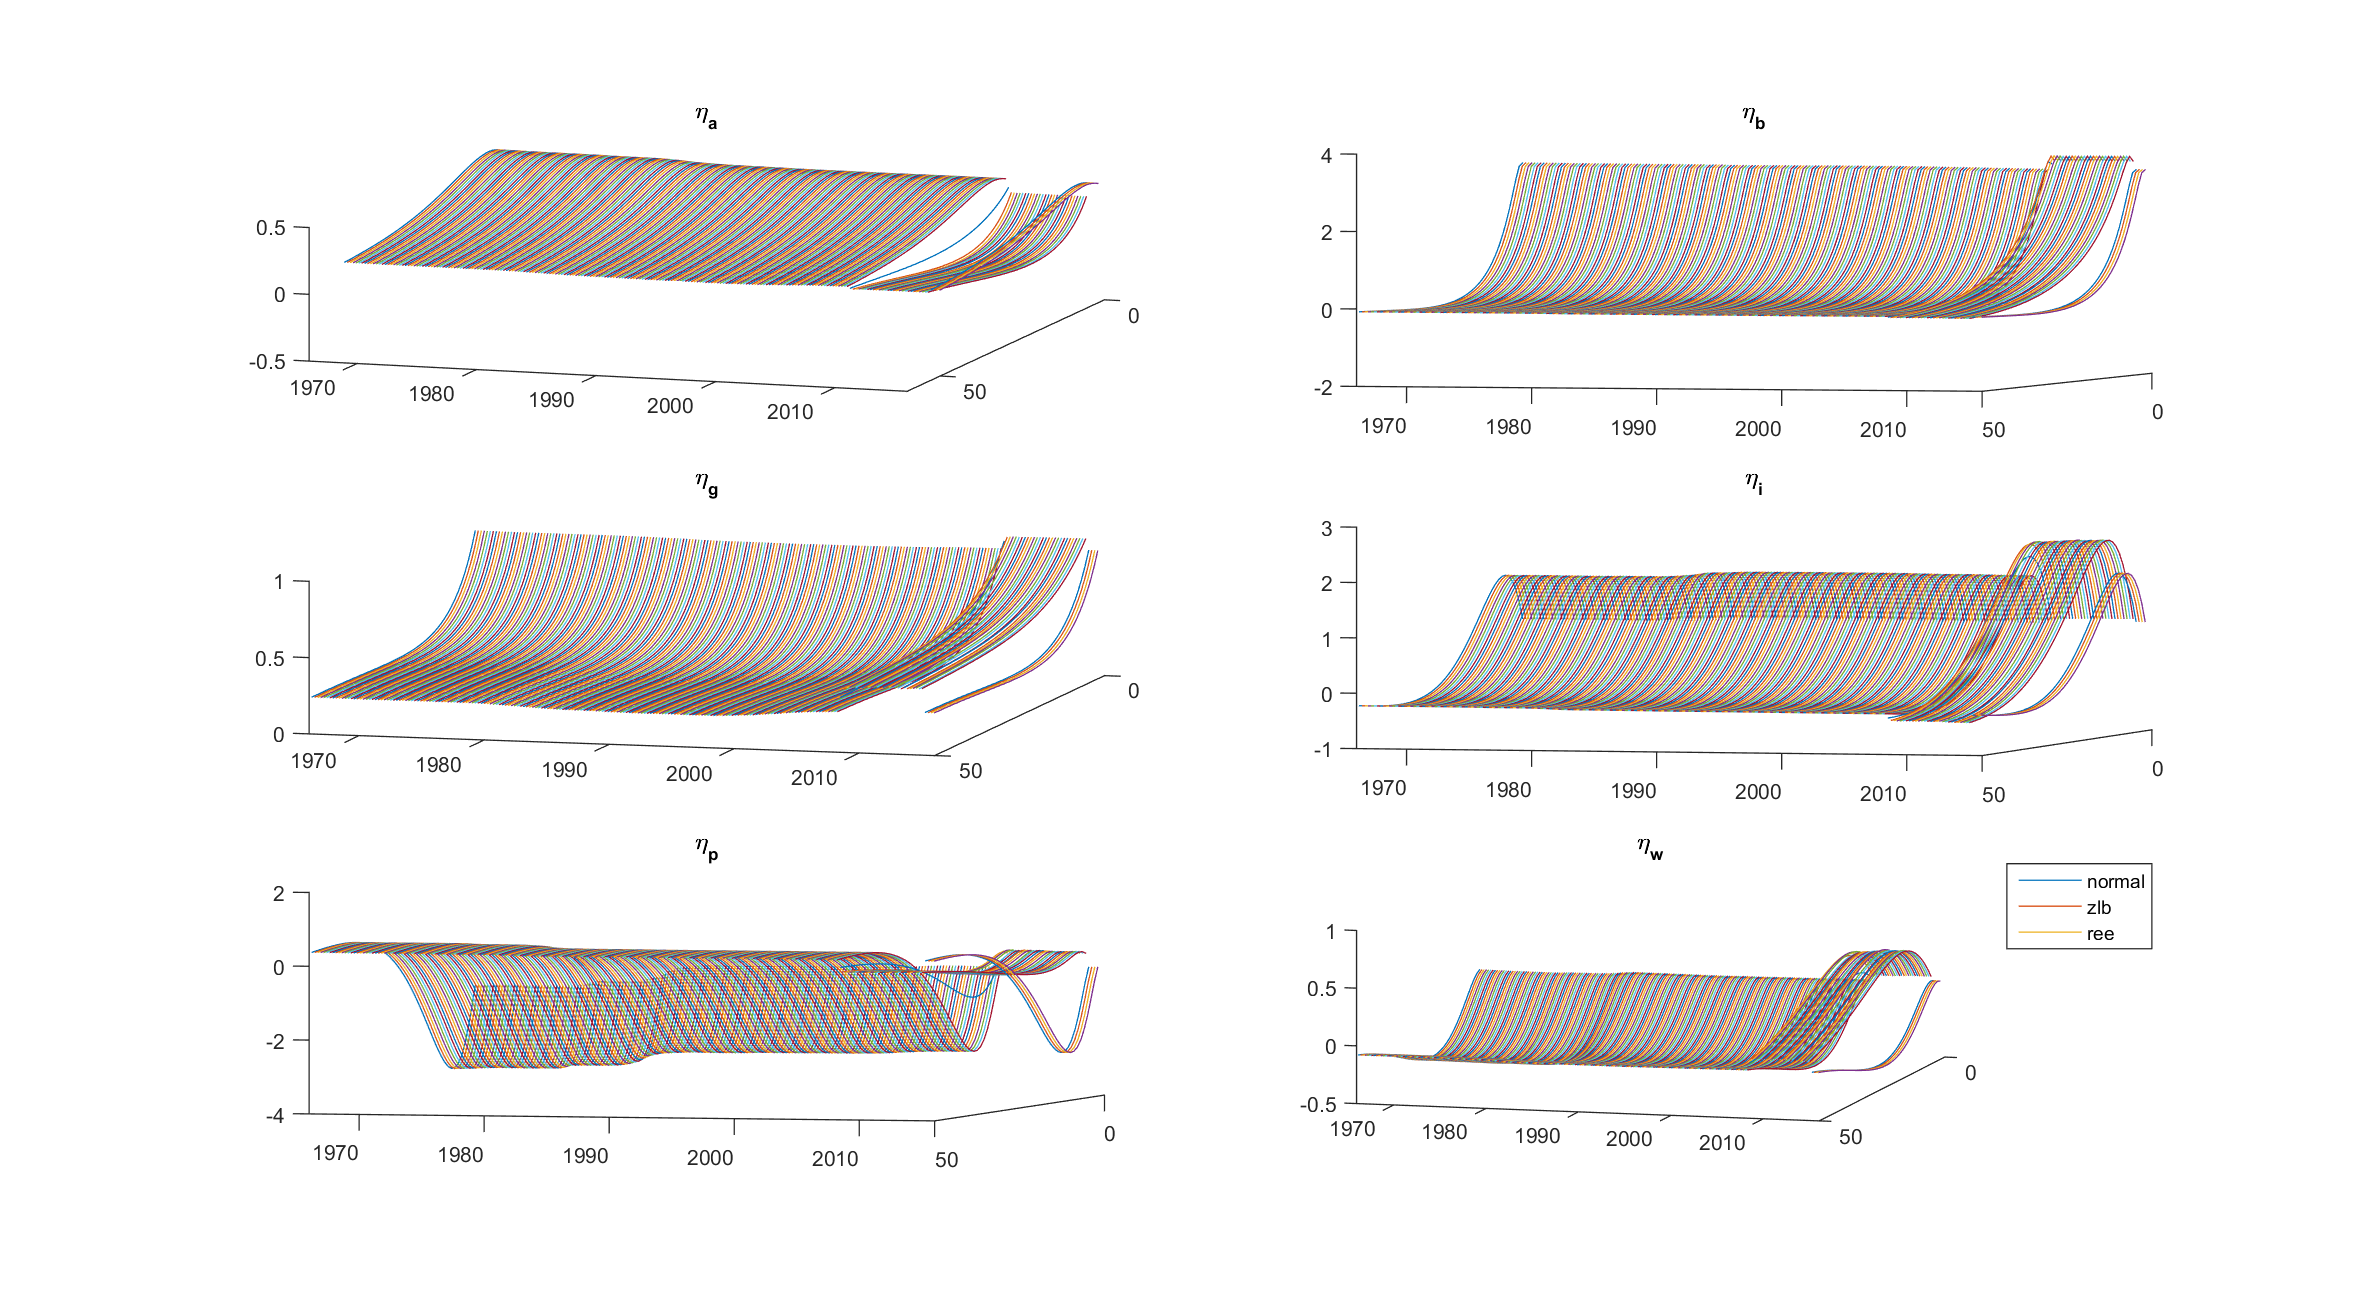
\includegraphics[scale=0.5]{MSV_impresp_output_3d.pdf}
\textbf{Inflation:}\\
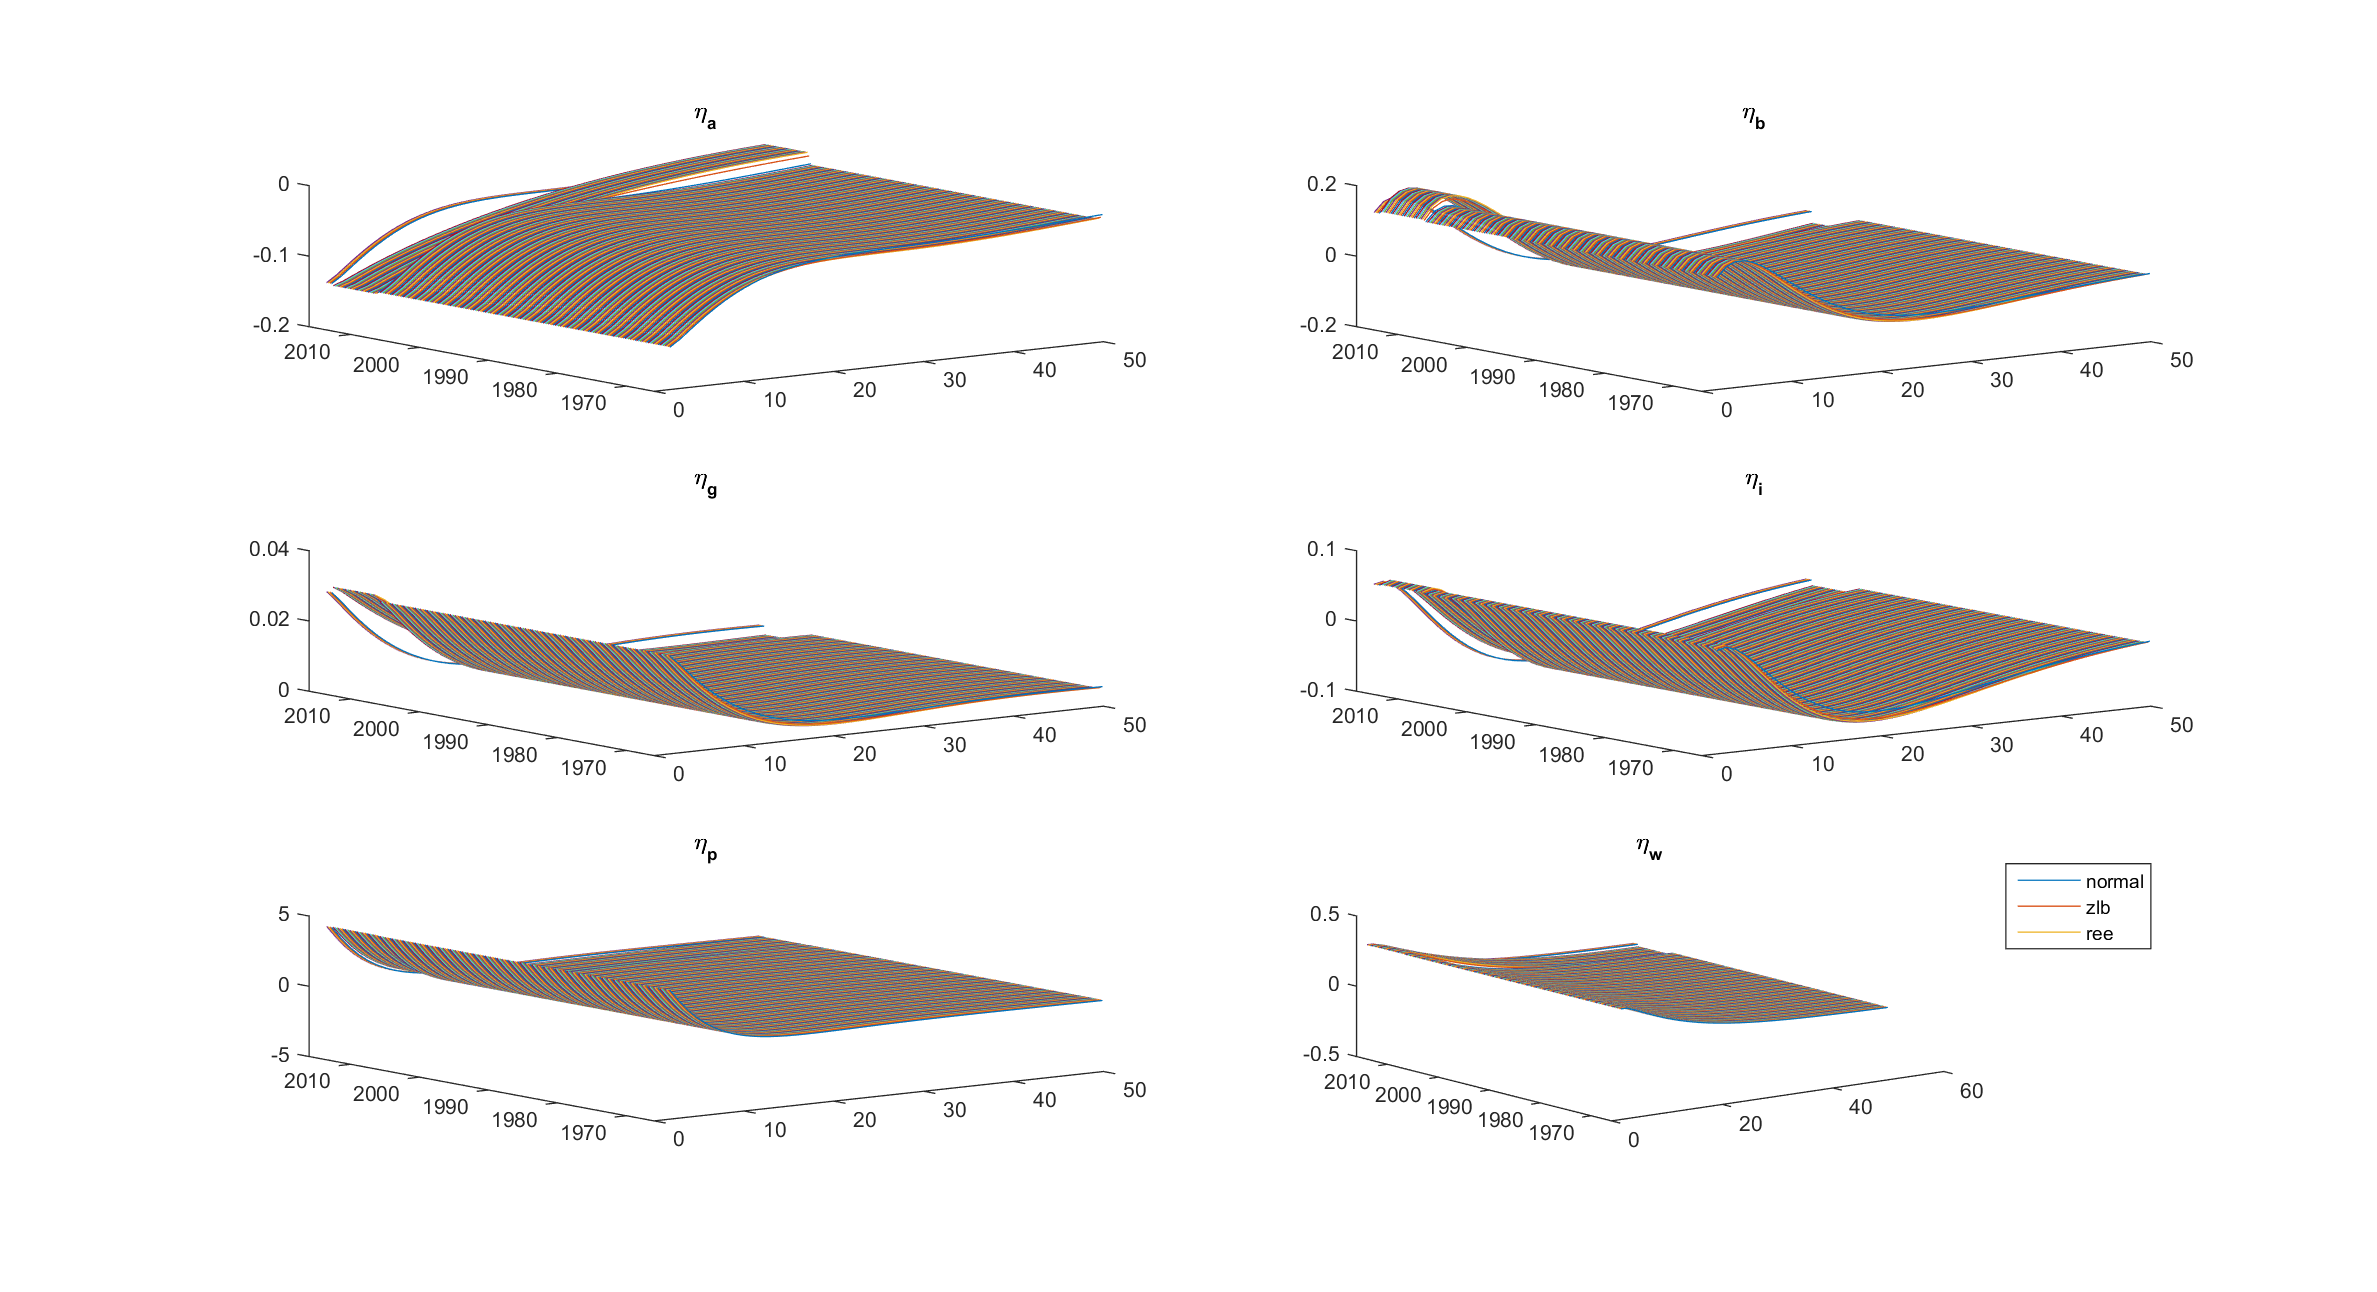
\includegraphics[scale=0.5]{MSV_impresp_pinf_3d.pdf}

\end{figure}


\end{document}

